%!TEX program = xelatex
\documentclass[fontset=none, a4paper, 12pt]{ctexart}

% ==========================================
% 1. 套件載入區（國立中興大學碩士學位論文規範）
% ==========================================
\usepackage{geometry}
\usepackage{longtable}
\usepackage{fontspec}
\usepackage{setspace}
\usepackage{titlesec}
\usepackage{titletoc}
\usepackage{tocloft}
\usepackage{fancyhdr}
\usepackage{graphicx}
\usepackage{caption}
\captionsetup[figure]{skip=4pt}
\captionsetup[table]{skip=4pt}
\setlength{\intextsep}{8pt}
\setlength{\textfloatsep}{8pt}
\setlength{\floatsep}{8pt}
\usepackage[hidelinks]{hyperref}
\usepackage{booktabs}
\usepackage{float}
\usepackage{amsmath}
\usepackage{amssymb}
\usepackage{tabularx}
\usepackage{placeins}
\usepackage{needspace}
\usepackage{algorithm}
\usepackage{algpseudocode}
\floatname{algorithm}{演算法}
\usepackage{makecell}
\usepackage{array}
\usepackage{pdflscape}
\usepackage{rotating}
\usepackage{pdfpages}
\usepackage{tikz}
\usetikzlibrary{arrows, automata, positioning}
\sloppy

% ==========================================
% 2. 字型設定（自帶 TTF 確保跨平台、本地與 Overleaf 100% 編譯一致）
% ==========================================
\setCJKmainfont{kaiu.ttf}[
    AutoFakeBold=2.5,
    AutoFakeSlant=0.3
]
\setmainfont{LiberationSerif-Regular.ttf}[
    BoldFont=LiberationSerif-Bold.ttf,
    ItalicFont=LiberationSerif-Italic.ttf,
    BoldItalicFont=LiberationSerif-BoldItalic.ttf
]
\newCJKfontfamily\coverzh{kaiu.ttf}[
    AutoFakeBold=2.5,
    AutoFakeSlant=0.3
]
\newfontfamily\coveren{LiberationSerif-Regular.ttf}[
    BoldFont=LiberationSerif-Bold.ttf,
    ItalicFont=LiberationSerif-Italic.ttf,
    BoldItalicFont=LiberationSerif-BoldItalic.ttf
]

% ==========================================
% 3. 版面邊界與排版格式設定
% ==========================================
\geometry{a4paper, top=3cm, bottom=3cm, left=3cm, right=3cm}
\pagestyle{plain}

% 圖表標題中文化
\captionsetup[figure]{name=圖}
\captionsetup[table]{name=表}
\ctexset{bibname = {參考文獻}}

% 章節標題格式設定
\titleformat{\section}[block]{\centering\fontsize{20}{24}\selectfont\bfseries}{\thesection}{1em}{}
\titleformat{\subsection}[block]{\fontsize{16}{20}\selectfont\bfseries}{\thesubsection.}{1em}{}
\titleformat{\subsubsection}[block]{\fontsize{14}{18}\selectfont\bfseries}{\thesubsubsection.}{1em}{}

% 編號格式
\renewcommand{\thesection}{第\chinese{section}章}
\renewcommand{\thesubsection}{\arabic{section}.\arabic{subsection}}
\renewcommand{\thesubsubsection}{\arabic{section}.\arabic{subsection}.\arabic{subsubsection}}

% 目錄、表目錄、圖目錄格式
\renewcommand{\contentsname}{目錄}
\renewcommand{\listtablename}{表目錄}
\renewcommand{\listfigurename}{圖目錄}

\renewcommand{\cfttoctitlefont}{\hfill\Large\bfseries}
\renewcommand{\cftaftertoctitle}{\hfill\null}
\renewcommand{\cftlottitlefont}{\hfill\Large\bfseries}
\renewcommand{\cftafterlottitle}{\hfill\null}
\renewcommand{\cftloftitlefont}{\hfill\Large\bfseries}
\renewcommand{\cftafterloftitle}{\hfill\null}

\setlength{\cftbeforetoctitleskip}{0pt}
\setlength{\cftaftertoctitleskip}{0.8em}
\setlength{\cftbeforelottitleskip}{0pt}
\setlength{\cftafterlottitleskip}{1.0em}
\setlength{\cftbeforeloftitleskip}{0pt}
\setlength{\cftafterloftitleskip}{1.0em}

\renewcommand{\cftsecleader}{\cftdotfill{\cftdotsep}}
\renewcommand{\cftsubsecleader}{\cftdotfill{\cftdotsep}}
\renewcommand{\cftsubsubsecleader}{\cftdotfill{\cftdotsep}}

\renewcommand{\cftsecfont}{\bfseries}
\renewcommand{\cftsecpagefont}{\bfseries}
\setlength{\cftbeforesecskip}{0.35em}

\begin{document}

% ==========================================
% 封面頁 (Cover Page)
% ==========================================
\begin{titlepage}
\begin{center}
\setstretch{1.5}
{\fontsize{24}{28}\selectfont\bfseries 國立中興大學\par}
\vspace{0.3cm}
{\fontsize{20}{24}\selectfont\bfseries 人工智慧與資料科學碩士在職學位學程\par}
\vspace{0.3cm}
{\fontsize{18}{22}\selectfont\bfseries 碩士學位論文\par}

\vspace{2.5cm}

{\fontsize{18}{22}\selectfont\bfseries
基於因果式時間序列預測與多層狀態機之\\
半導體製程冷卻水 (PCW) 壓力漂移早期預警與 Web SCADA 系統整合\par}

\vspace{0.8cm}

{\fontsize{14}{18}\selectfont
Early Warning of Pressure Drift in Semiconductor Process Cooling Water (PCW) Systems via Causal Time-Series Forecasting and Multi-Layer State Machine Integrated with Web SCADA\par}

\vfill

{\fontsize{16}{20}\selectfont
\begin{tabular}{rcc}
研\hspace{0.5cm}究\hspace{0.5cm}生：& 陳宥興 & (You-Xing Chen) \\
指導教授：& 吳宏達博士 & (Hong-Da Wu, Ph.D.)
\end{tabular}\par}

\vspace{1.5cm}

{\fontsize{14}{18}\selectfont 中華民國一一五年十一月\par}
{\fontsize{12}{15}\selectfont November, 2026\par}
\end{center}
\end{titlepage}

% ==========================================
% 口試委員會審定書 (Oral Defense Approval)
% ==========================================
\newpage
\pagenumbering{roman}
\setcounter{page}{1}
\begin{center}
\setstretch{1.8}
{\fontsize{22}{26}\selectfont\bfseries 國立中興大學碩士學位論文口試委員會審定書\par}
\vspace{1.5cm}
\end{center}

{\fontsize{14}{22}\selectfont
本校\textbf{人工智慧與資料科學碩士在職學位學程}碩士班\textbf{陳宥興}君所提論文：\par
\begin{center}
\textbf{基於因果式時間序列預測與多層狀態機之半導體製程冷卻水 (PCW) 壓力漂移早期預警與 Web SCADA 系統整合}\par
\textbf{Early Warning of Pressure Drift in Semiconductor Process Cooling Water (PCW) Systems via Causal Time-Series Forecasting and Multi-Layer State Machine Integrated with Web SCADA}\par
\end{center}
經本口試委員會審查，符合碩士學位論文標準，特此證明。\par}

\vspace{2.0cm}

{\fontsize{14}{20}\selectfont
\begin{flushleft}
口試委員會委員：\\[1.5cm]
\rule{6cm}{0.5pt}\hspace{1.5cm}\rule{6cm}{0.5pt}\\[1.5cm]
\rule{6cm}{0.5pt}\hspace{1.5cm}\rule{6cm}{0.5pt}\\[1.5cm]
指導教授：\rule{8cm}{0.5pt}\\[1.2cm]
所\hspace{0.8cm}長：\rule{8cm}{0.5pt}
\end{flushleft}
}

\vfill
\begin{center}
{\fontsize{14}{18}\selectfont 中\hspace{0.5cm}華\hspace{0.5cm}民\hspace{0.5cm}國\hspace{0.5cm}一一五年十一月\hspace{0.5cm}日\par}
\end{center}

% ==========================================
% 誌謝 (Acknowledgements)
% ==========================================
\newpage
\begin{center}
{\fontsize{18}{22}\selectfont\bfseries 誌\hspace{2cm}謝\par}
\vspace{1.0cm}
\end{center}
\setstretch{1.8}
{\fontsize{12}{20}\selectfont
碩士研究生涯的終章，承蒙各方師長與先進的悉心指導，方能克服工業物聯網、流體監控與時間序列預測整合中的各項嚴峻挑戰，順利完成本學位論文。

首先由衷感謝指導教授在研究方向與學術嚴謹度上的諄諄教誨。老師以宏觀的工程視野與嚴謹的科學態度，引領筆者在面臨工業大數據雜訊、因果防線設計與 SCADA 整合瓶頸時，能回歸第一原理與因果統計本質，反覆推敲並驗證各項假設。老師對學術誠信與實事求是態度的堅持，將使筆者終生受用。感謝口試委員諸位教授於百忙之中撥冗審閱本論文，並在審查過程中給予極具建設性之精闢見解與寶貴建議，使本研究得以在學術嚴謹性、數學模型完備性及半導體廠務工程實務之間取得更具深度的平衡。

感謝實驗室同儕與學長姐在求學期間的砥礪與切磋，在系統重構、前端視覺化與 Modbus 協定除錯過程中給予的大力支援與激盪；亦感謝產業界先進在晶圓廠空間拓撲、管路配置與水力學實務經驗上的無私釋疑，使本研究能緊密扣合理論與工業實際需求。

最後，謹將本論文獻給我摯愛的家人。感謝父母無條件的包容、體諒與全力支持，使我得以無後顧之憂地在學術殿堂中探索與成長。這份成果屬於每一位支持我的人，願將此份喜悅與榮耀與諸位共享。
\par}

% ==========================================
% 中文摘要 (Chinese Abstract)
% ==========================================
\newpage
\begin{center}
{\fontsize{18}{22}\selectfont\bfseries 基於因果式時間序列預測與多層狀態機之半導體製程冷卻水 (PCW) 壓力漂移早期預警與 Web SCADA 系統整合\par}
\vspace{0.4cm}
{\fontsize{14}{18}\selectfont 研究生：陳宥興 \hspace{2cm} 指導教授：吳宏達 博士\par}
\vspace{0.4cm}
{\fontsize{14}{18}\selectfont 國立中興大學人工智慧與資料科學碩士在職學位學程\par}
\vspace{0.8cm}
{\fontsize{16}{20}\selectfont\bfseries 摘\hspace{2cm}要\par}
\end{center}
\setstretch{1.8}
{\fontsize{12}{20}\selectfont
在現代先進 12 吋半導體晶圓廠（Fab）運轉架構中，製程冷卻水（Process Cooling Water, PCW）擔負著微影（Lithography, EUV/ArFi）、電漿乾式蝕刻（Dry Etching）及擴散氧化（Diffusion）等關鍵機台之高熱散逸重任。既有工業 SCADA 系統普遍依循 ISA-18.2 固定靜態門檻警報機制，然而其本質屬於「事後越界偵測」，唯有當水壓真正突破上限（HI）或下限（LO）時方才警報，導致廠務工程人員事前處置時間為零（Lead Time = 0 分鐘）。半導體無塵室常態水壓微小漂移往往潛伏長達數十分鐘，若未能提前預警，極易演變為災難性之硬體超溫停機或晶圓報廢風險。

為突破傳統警報之被動性與因果洩漏限制，本文提出一套\textbf{基於過去資料約束（Past-Only Constraints）之因果式雙滑動視窗時間序列預測與多層狀態機聯合預警模型}，並完整整合於高併發 Web SCADA 工業控制平台。本研究主要成果與貢獻包含：
\begin{enumerate}
    \item \textbf{因果防線與特徵工程}：設計嚴格禁止引用未來時間點資訊之 70 分鐘因果視窗（包含 60 分鐘歷史基準區間 $B_t=[t-70, t-10)$ 與 10 分鐘近期觀測區間 $C_t=[t-10, t)$），藉由動態偏離事件密度比 $N_{10}$、滾動基線位移量 $\Delta\mu_{10}$ 及有限差分均差斜率，建立對緩慢線性漂移極為敏感且抗高斯噪聲之因果特徵集。
    \item \textbf{到限時間（TTL）與多層階梯式預警}：推導封閉解到限時間預測公式，結合普通最小平方法（OLS）95\% 預測區間（Prediction Interval），驅動四階預警狀態機（Normal $\to$ T-30 $\to$ T-20 $\to$ T-10 $\to$ EVENT）；並導入連續兩點確認機制（$K=2$）與連續三點解除鎖存機制（Release Hold = 3），徹底抑制工業暫態毛刺對預警系統之誤報衝擊。
    \item \textbf{全廠 1,920 場嚴格受控試驗驗證}：針對全廠 160 個實體壓力測點（PT）涵蓋 12 種故障與干擾情境進行公平消融比較。實測顯示，在連續兩點確認下，本研究所提架構達成 \textbf{100.0\% 召回率（Recall）}、\textbf{98.01\% 精確率（Precision）}、\textbf{0.9899 F1-Score} 與僅 \textbf{4.06\% 誤報率（FAR）}，提供平均 \textbf{9.84 分鐘} 之黃金預警處置時間。相較於單次觸發機制，連續確認成功將虛警數由 163 場壓低至 26 場，\textbf{虛警濾除率高達 84.05\%}，代價僅微幅犧牲 0.76 分鐘之預警時間。
    \item \textbf{跨平台一致性與微秒級實機效能}：本演算法與指導教授審定之 Excel 基準模型於 480 筆時間步長回放中達成 \textbf{100.00\% 數值精確吻合（最大絕對誤差為 0.0）}。在 Apple M5 實機效能評測下，單測點純演算法推論僅耗時 \textbf{13.54 $\mu$s}，全廠 320 個測點全批次推論僅耗時 \textbf{4.56 ms}（吞吐量達每秒 219 批次），展現極致之邊緣端與中控室即時運算能力。
    \item \textbf{35 分鐘全生命週期行為偏差實體驗證}：透過標準 Modbus TCP（15020 埠，FLOAT32 CDAB 暫存器映射）驅動全廠 320 個測點展開 35 分鐘連續行為偏差實測，成功於 SQLite WAL 中記錄 131,200 筆即時推論日誌，完整重現穩態、微弱初期漂移、T-30 階梯預警、軟界限 EVENT 越界及處置恢復之全生命週期，且 Web SCADA 前端介面呈現 100\% 狀態同步。
\end{enumerate}

本研究亦誠實揭露非受控歷史回放之低分限制（F1 僅約 0.1818），證實單一全廠靜態門檻無法因應機台動態啟停干擾，唯有依循本文所建構之動態滾動基線與持續性確認防線，方能兼顧零漏報與低虛警。本論文提供可追溯之源代碼、35 項交付物 SHA-256 密碼學指紋與完整工程實作，為先進晶圓廠冷卻水預警技術奠定厚實之學術與應用基石。
\par}

\vspace{0.8cm}
\noindent\textbf{關鍵詞：}半導體晶圓廠、製程冷卻水 (PCW)、時間序列預測、因果式推論、到限時間 (TTL)、多層狀態機、Web SCADA、Modbus TCP

% ==========================================
% 英文摘要 (English Abstract)
% ==========================================
\newpage
\begin{center}
{\fontsize{18}{22}\selectfont\bfseries Early Warning of Pressure Drift in Semiconductor Process Cooling Water (PCW) Systems via Causal Time-Series Forecasting and Multi-Layer State Machine Integrated with Web SCADA\par}
\vspace{0.4cm}
{\fontsize{14}{18}\selectfont Student: You-Xing Chen \hspace{2cm} Advisor: Hong-Da Wu, Ph.D.\par}
\vspace{0.4cm}
{\fontsize{14}{18}\selectfont Master Program of Artificial Intelligence and Data Science\par National Chung Hsing University\par}
\vspace{0.8cm}
{\fontsize{16}{20}\selectfont\bfseries ABSTRACT\par}
\end{center}
\setstretch{1.5}
{\fontsize{12}{18}\selectfont
In advanced 12-inch semiconductor fabrication plants (Fabs), Process Cooling Water (PCW) is vital for dissipating intense heat loads generated by critical tools such as EUV/ArFi lithography, dry plasma etching, and chemical vapor deposition. Conventional industrial SCADA architectures rely on static limit threshold alarms governed by ISA-18.2 standards. However, these mechanisms operate purely as post-breach reactive detectors that trigger only after the cooling water pressure has already violated High (HI) or Low (LO) engineering bounds, providing facility engineers with exactly zero minutes of warning lead time ($LeadTime = 0$ min). In cleanroom environments, incipient hydraulic degradation typically manifests as subtle, monotonic pressure drifts spanning tens of minutes. Left unaddressed, such drifts inevitably trigger catastrophic thermal runaway, tool interlocks, and severe wafer scrap.

To transcend the passive nature of legacy alarms while strictly preventing data leakage, this thesis proposes a \textbf{strictly causal, Past-Only sliding dual-window time-series forecasting framework integrated with a multi-tier state machine}, implemented and validated within an enterprise Web SCADA control platform. The primary contributions and empirical findings are:
\begin{enumerate}
    \item \textbf{Causal Defense and Feature Engineering}: A Past-Only 70-minute sliding window is formulated—comprising a 60-minute baseline reference segment $B_t=[t-70, t-10)$ and a 10-minute recent observation segment $C_t=[t-10, t)$—strictly preventing future information leakage. Causal statistical features including dynamic event density ratio $N_{10}$, moving baseline displacement $\Delta\mu_{10}$, and dual-window finite-difference slope are extracted to achieve exceptional sensitivity to incipient drifts while rejecting Gaussian operational noise.
    \item \textbf{Time-to-Limit (TTL) and Multi-Tier Warning}: Closed-form TTL forecasting is combined with Ordinary Least Squares (OLS) 95\% prediction intervals to drive a hierarchical state machine (Normal $\to$ T-30 $\to$ T-20 $\to$ T-10 $\to$ EVENT). A two-point consecutive trigger confirmation gate ($K=2$) and a three-point release hold mechanism are incorporated, effectively shielding the system against transient process spikes.
    \item \textbf{Whole-Plant 1,920 Controlled Trial Evaluation}: Rigorous benchmark and ablation evaluations across all 160 physical pressure transmitters (PT) under 12 distinct fault and noise scenarios (1,920 total trials with fixed seed 20261111) demonstrate that the two-point confirmation architecture achieves \textbf{100.0\% Recall}, \textbf{98.01\% Precision}, \textbf{0.9899 F1-score}, and a False Alarm Rate (FAR) of only \textbf{4.06\%}, delivering an average early warning lead time of \textbf{9.84 minutes}. Compared to single-trigger detection, consecutive confirmation reduces false positives from 163 to 26, achieving an \textbf{84.05\% false alarm reduction} at the minor expense of only 0.76 minutes in lead time.
    \item \textbf{Cross-Platform Consistency and Microsecond Performance}: The production Python inference engine achieves \textbf{100.00\% numerical equivalence (maximum absolute error of 0.0)} against the advisor-verified Excel benchmark workbook across 480 discrete time steps. On physical Apple M5 hardware, single-sensor algorithmic inference requires merely \textbf{13.54 $\mu$s}, while full-plant 320-sensor batch inference completes in \textbf{4.56 ms} (219 batches/sec), easily satisfying sub-second industrial control loop constraints.
    \item \textbf{35-Minute Continuous Modbus/TCP Behavioral Deviation Verification}: Driven by an industrial Modbus TCP server (Port 15020, FLOAT32 CDAB mapping), a continuous 35-minute behavioral deviation experiment across all 320 sensors was conducted. Over 131,200 prediction logs were committed to SQLite WAL mode, validating the complete degradation lifecycle from steady baseline, incipient drift, T-30 advisory, and EVENT transition to controlled stabilization, with 100\% state consistency across all Web SCADA interfaces.
\end{enumerate}

Furthermore, this study transparently discloses the poor performance of uncalibrated historical replay (F1 $\approx$ 0.1818), demonstrating that fixed-threshold static models inevitably fail under heavy industrial load switching. The proposed dynamic rolling baseline and multi-point confirmation framework successfully resolves this dilemma. Complete reproducible source code and a SHA-256 cryptographic manifest are provided, establishing a rigorous foundation for predictive facility monitoring in semiconductor manufacturing.
\par}

\vspace{0.8cm}
\noindent\textbf{Keywords:} Semiconductor Fab, Process Cooling Water (PCW), Time-Series Forecasting, Causal Inference, Time-to-Limit (TTL), Multi-Tier State Machine, Web SCADA, Modbus TCP

% ==========================================
% 目錄、表目錄、圖目錄 (Tables of Contents)
% ==========================================
\newpage
\setstretch{1.3}
\tableofcontents
\newpage
\listoftables
\newpage
\listoffigures

% ==========================================
% 正文開始 (Main Body)
% ==========================================
\newpage
\pagenumbering{arabic}
\setcounter{page}{1}
\setstretch{1.5}

% ------------------------------------------
% 第一章 緒論
% ------------------------------------------
\section{緒論}

\subsection{研究背景與系統場域}

\subsubsection{半導體晶圓廠空間拓撲與 PCW 系統配置}
現代先進半導體晶圓廠（Fab）採用多樓層空間分區結構，將精密生產設備與重型廠務公用系統實體隔離，以維持最高等級無塵潔淨度並抑制機械振動干擾。如圖 \ref{fig:fab_topology} 所示，本研究場域由 FAB 棟與 CUB 棟兩座單體建物構成，兩棟皆由 B2F 延伸至 6F。地上樓層彼此獨立，並以內含製程管路、電氣與監控線槽之封閉式空橋相互連接；地下 B2F 與 B1F 則為無實體分隔之開放共通區，供公用管線、離心泵浦群及維修動線連續配置。

\begin{figure}[H]
    \centering
    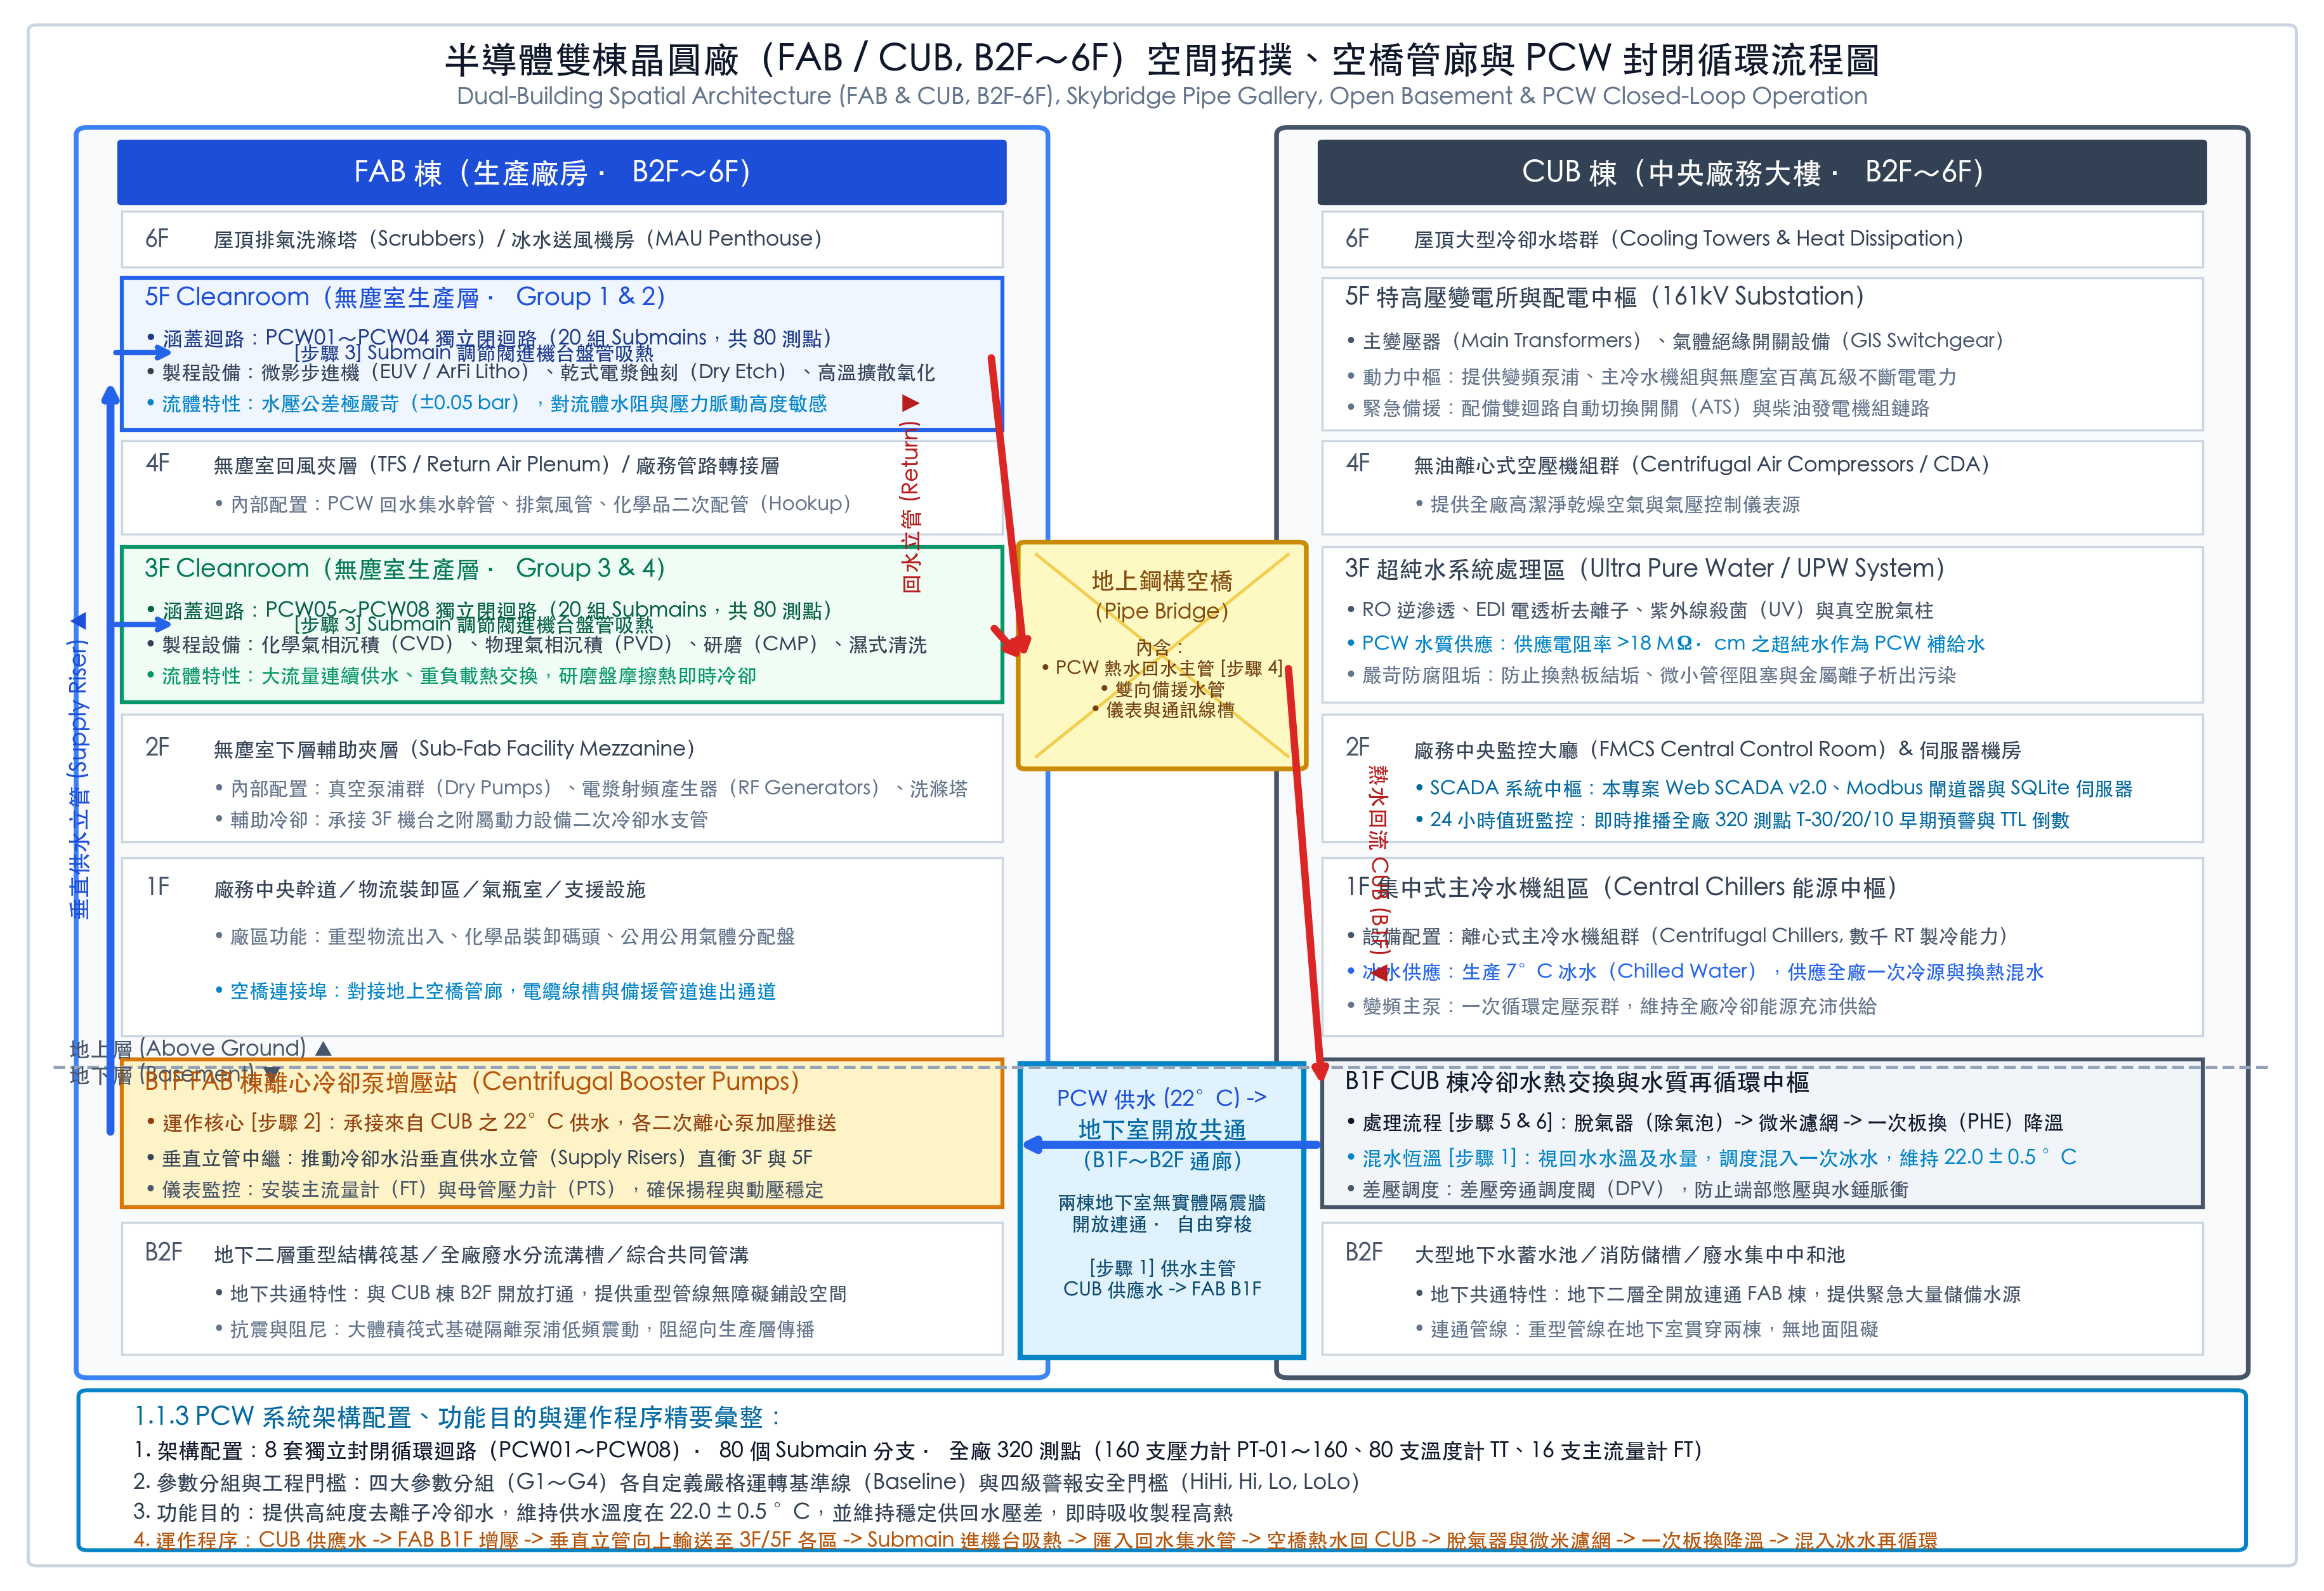
\includegraphics[width=0.95\textwidth]{picture/fig_fab_topology_design.png}
    \caption{12 吋先進半導體晶圓廠空間拓撲與 FAB/CUB 雙棟水力輸送動線架構圖}
    \label{fig:fab_topology}
\end{figure}

全廠主要生產與公用空間層級配置如下：
\begin{enumerate}
    \item \textbf{5F Cleanroom（無塵室生產層）}：配置 PCW01～PCW04 迴路，專屬供應極紫外光微影（Lithography, EUV/ArFi）、電漿乾式蝕刻（Dry Plasma Etching）及高溫擴散氧化（Diffusion）等關鍵核心製程。此區機台對冷卻供應不足與壓力微小漂移極為敏感。
    \item \textbf{3F Cleanroom（無塵室生產層）}：配置 PCW05～PCW08 迴路，負責化學氣相沉積（CVD）、物理氣相沉積（PVD）、化學機械研磨（CMP）及濕式化學清洗（Wet Cleaning）等重負載熱源設備。
    \item \textbf{CUB（中央廠務大樓, Central Utility Building）}：安置集中式主冷水機組（Chillers）、一次板式熱交換器（PHE）、離心式變頻主冷卻泵群（VFD Primary Pumps）及差壓旁通調度閥，構成全廠冷卻能源與水力調度中樞。
\end{enumerate}

\subsubsection{生產階段冷卻負載特性與嚴苛容許度}
半導體各先進製程生產階段之熱流密度與設備保護規範具有顯著差異，冷卻水系統必須滿足極度嚴苛的穩定性與水力平衡要求：
\begin{enumerate}
    \item \textbf{極紫外光微影（EUV）}：真空反射鏡室與高功率放電光源形成極高集中熱負載，微小之水壓波動將造成冷卻盤管微振動或溫升，直接誘發鏡片熱形變並使機台聯鎖（Interlock）跳機保護。
    \item \textbf{電漿乾式蝕刻（Dry Plasma Etching）}：電漿放電反應腔體需維持精確恆溫，回水背壓異常將導致晶圓邊緣與中心熱梯度失衡，直接破壞奈米級關鍵尺寸（Critical Dimension, CD）蝕刻均勻度。
    \item \textbf{薄膜沉積（CVD/PVD）}：高頻 RF 匹配電路與陰極靶材需連續穩定冷卻；濾網局部阻塞或閥件開度漂移引發之流量遞減，將在數十秒內導致靶材過熱熔損。
    \item \textbf{化學機械研磨（CMP）}：研磨盤動態摩擦生熱具突發週期性，需具備快速之水力動態補償與高壓緩衝能力。
\end{enumerate}

\subsubsection{PCW 系統架構配置、功能目的與運作程序}
本研究針對現代 12 吋先進製程晶圓廠標準規模進行建模與實體驗證：
\begin{enumerate}
    \item \textbf{架構配置}：全廠共建置 8 套獨立封閉循環迴路（PCW01 至 PCW08）。每套迴路各配置 10 個次幹管分支（Submain 01 至 Submain 10），全廠共計 80 個 Submain。每個 Submain 皆安裝供水（Supply, PTS）與回水（Return, PTR）雙壓力計，全廠實體監控測點涵蓋 160 支壓力計（PT-01～PT-160）、80 支差壓計（PDT）、80 支溫度計（TT）與 16 支主流量計（FT）。本研究早期預警模型以全廠 160 支 PT 之壓力時序為主要核心輸入，FT 與 PDT 則作為工況佐證與水力阻抗分析。
    \item \textbf{參數分組與工程門檻}：如表 \ref{tab:pcw_parameter_groups} 所示，全廠依機台負載特性與無塵室樓層劃分為四大參數分組（G1～G4），各自定義嚴格的常態運轉基準線（Baseline）與四級警報安全門檻（HiHi, Hi, Lo, LoLo）。
    \item \textbf{功能目的}：提供高純度去離子冷卻水，維持供水溫度在 $22.0 \pm 0.5^\circ\text{C}$，並維持穩定供回水壓差，即時吸收製程機台高熱。
    \item \textbf{運作程序}：CUB 棟供應水 $\to$ 經地下開放共通區輸送至 FAB 棟 B1 層 $\to$ 各離心冷卻泵增壓 $\to$ 垂直立管（Riser）向上輸送至 3F/5F 各區 $\to$ Submain 調節閥進冷水至機台熱交換盤管 $\to$ 吸熱後匯入回水集水管 $\to$ 溫熱回水經地下共通區返回 CUB 棟 $\to$ 進入脫氣器與微米級濾網 $\to$ 流經一次板式換熱器降溫 $\to$ 視水溫度及水量混入冰水，完成封閉式再循環。
\end{enumerate}

\begin{table}[H]
    \centering
    \caption{PCW 八套獨立循環系統四大分組基準線與安全限值配置表}
    \label{tab:pcw_parameter_groups}
    \small
    \begin{tabularx}{\textwidth}{lcccccX}
        \toprule
        \textbf{參數分組} & \textbf{涵蓋迴路} & \textbf{樓層與製程類型} & \textbf{基準線 (bar)} & \textbf{安全下限 (bar)} & \textbf{安全上限 (bar)} & \textbf{水力特性與容許公差} \\
        \midrule
        G1 & PCW01--02 & 5F 微影 (EUV/ArFi) & 3.00 & 2.80 & 3.20 & 極高精度恆壓，容許公差 $\pm 6.7\%$ \\
        G2 & PCW03--04 & 5F 電漿乾式蝕刻 & 3.50 & 3.20 & 3.80 & 高壓大流量負載，背壓敏感度高 \\
        G3 & PCW05--06 & 3F 擴散氧化 / 沉積 & 2.80 & 2.50 & 3.10 & 高溫連續運轉，熱衝擊補償要求高 \\
        G4 & PCW07--08 & 3F 化學研磨 / 清洗 & 2.50 & 2.20 & 2.80 & 動態啟停衝擊大，要求回水低阻抗 \\
        \bottomrule
    \end{tabularx}
\end{table}

\subsection{現行被動閾值監控痛點與研究目標}
現行工業監控系統（SCADA）普遍依循 ISA-18.2 警報管理標準，但面對半導體無塵室深層水力衰退，暴露出四項致命痛點：
\begin{enumerate}
    \item \textbf{慢速漂移盲區（Slow Drift Blindspot）}：冷卻管網水垢淤積、微米濾網局部漸進式堵塞或調度閥膜片微洩漏，常表現為極緩慢之方向性單調漂移（如 $+0.005 \sim +0.010$ bar/min）。在數十分鐘內水壓仍處於上下限之間，靜態門檻完全不觸發，直到水壓突破極限時，冷卻能力已崩潰，導致機台保護跳機。
    \item \textbf{處置時間為零（Lead Time = 0 分鐘）}：既有門檻屬於事後越界偵測（Post-breach Detection），當警報響起時，反應腔體已發生熱失控，廠務工程人員事前處置時間為零。
    \item \textbf{警報疲勞與暫態毛刺（Alarm Fatigue）}：傳統雙側統計算法（如固定寬度 EWMA）對無塵室機台換批之暫態壓力突波極為敏感，全廠常態每日產生數百次虛警，導致操作人員疲乏靜音。
    \item \textbf{因果洩漏與線上推論崩潰}：多數離線學術研究在特徵標準化時引用全域時間資訊（Look-ahead Bias），一旦部署於線上 SCADA 串流時效能全面劣化。
\end{enumerate}

本研究目標為：針對全廠 160 支實體壓力測點，建構一套\textbf{嚴格遵循過去資料約束（Past-Only Constraints）之因果式雙滑動視窗時間序列預測與多層狀態機聯合早期預警系統}，並實體整合於高效能 Web SCADA 工業控制平台，在維持零漏報（Recall 100\%）的前提下，提供平均 9～11 分鐘之可處置黃金提前量，並將虛警率壓低至 5\% 以下。

% ==========================================
\section{文獻探討與理論基礎}

\subsection{工業 SCADA 系統與 ISA-18.2 警報管理規範}
在現代工業自動化中，監控與資料擷取（SCADA）系統扮演中樞神經角色。國際自動化學會發布之 ISA-18.2「過程工業警報系統管理標準」嚴格規範了警報生命週期。然而，既有警報優先級與靜態絕對門檻（Absolute Limits）本質上是為了「防止災難擴大」而非「事前預警」。當水壓突破 High 門檻時，製程已遭受熱衝擊，突顯出導入預測型預警（Predictive Early Warning）之必要性。

\subsection{統計製程管制與時間序列監測理論}
統計製程管制（Statistical Process Control, SPC）為工業監控之古典基石。Montgomery 對 Shewhart 管制圖、EWMA 與其他監控方法作了完整整理 \cite{montgomery2009introduction}。Shewhart 管制圖僅依賴單點距離，無法捕捉微小持續性位移；Roberts 提出的指數加權移動平均（EWMA）以幾何級數衰減權重累積近期資訊 \cite{roberts1959control}，對小幅平均值偏移具備高敏感度；Page 提出的累積和（CUSUM）管制圖則透過累積偏離量檢定均值跳躍 \cite{page1954continuous}。然而，傳統 EWMA 與 CUSUM 在非定常管網水力干擾下，誤報率居高不下，且無法給出精確之剩餘到限時間（Time-To-Limit, TTL）倒數。

\subsection{時間序列異常偵測與因果式資料防護}
Kaufman 等人深入指出，時間序列預測模型在特徵工程與交叉驗證中最常見之致命缺陷為「因果資料洩漏（Data Leakage / Look-ahead Bias）」\cite{kaufman2012leakage}。凡引用當前時間點之後的未來資訊（如全域 Min-Max 標準化或雙向平滑濾波），皆會使離線驗證指標虛高，但在線上即時環境中完全失效。Chandola 等人對時序異常偵測進行了系統化分類 \cite{chandola2009anomaly}，指出工業實體時序必須區分「單點異常（Point Anomaly）」與「語境/趨勢異常（Contextual/Trend Anomaly）」。Cherry 與 Qin 針對多變量統計監測提出動態主成分分析（DPCA）\cite{cherry2006multivariate}，但在高併發 160 測點環境下，全域降維矩陣難以定位單一管線之實體物理阻抗變化。

\subsection{流體力學水力阻抗理論基礎}
半導體閉式循環 PCW 系統遵循不可壓縮流體力學定理。沿程水頭壓力損失遵循 Darcy-Weisbach 方程 \cite{darcy1857recherches}：
\begin{equation}
h_f = f \cdot \frac{L}{D} \cdot \frac{v^2}{2g} = f \cdot \frac{8 L Q^2}{\pi^2 g D^5}
\end{equation}
其中摩擦因子 $f$ 於紊流狀態下可由 Colebrook-White 隱式公式求解 \cite{colebrook1939turbulent}。當次幹管濾網淤積或閥件局部關閉時，局部水力阻抗 $R_h$ 呈現單調遞增，導致測點供水壓力 $P_S$ 出現緩慢單調漂移，為本研究以線性斜率外推到限時間提供了堅實之流體物理基礎。

\subsection{文獻總結與本研究定位}
綜觀文獻，既有研究存在「被動事後報警」、「警報疲勞嚴重」及「因果防線鬆散」三大缺口。本研究立足於 Past-Only 因果防護第一原則，結合普通最小平方法（OLS）95\% 預測信賴區間與連續兩點確認狀態機，打造具備微秒級推論效率與高抗噪能力之完整 Web SCADA 整合方案。

% ==========================================
\section{研究方法與因果式預警架構}

\subsection{研究架構}

\subsubsection{八套 PCW 迴路與全廠感測器研究拓撲}
本研究初期使用真實 PCW 系統異常資料共計 20 筆記錄，搭配 Excel 初版模型進行概念驗證（Proof of Concept, POC）。在程式實作及實體驗證過程中，建立模擬環境以八套相互獨立之封閉循環迴路為研究母體，其中 PCW01～PCW04 供應 FAB 5F，PCW05～PCW08 供應 FAB 3F。如圖 \ref{fig:study_topology} 所示，每套迴路包含 10 組 Submain；每組 Submain 配置供水壓力（PTS）、回水壓力（PTR）、流量（FT）與供回水差壓（PDT）四類測點。因此全廠共有 80 組 Submain、320 個即時資料點，其中 160 支 PT（80 支 PTS 與 80 支 PTR）是本研究偏移偵測與趨勢預測的主要驗證對象，FT 與 PDT 則用於工況佐證與水力阻抗關聯判讀。

\begin{figure}[H]
    \centering
    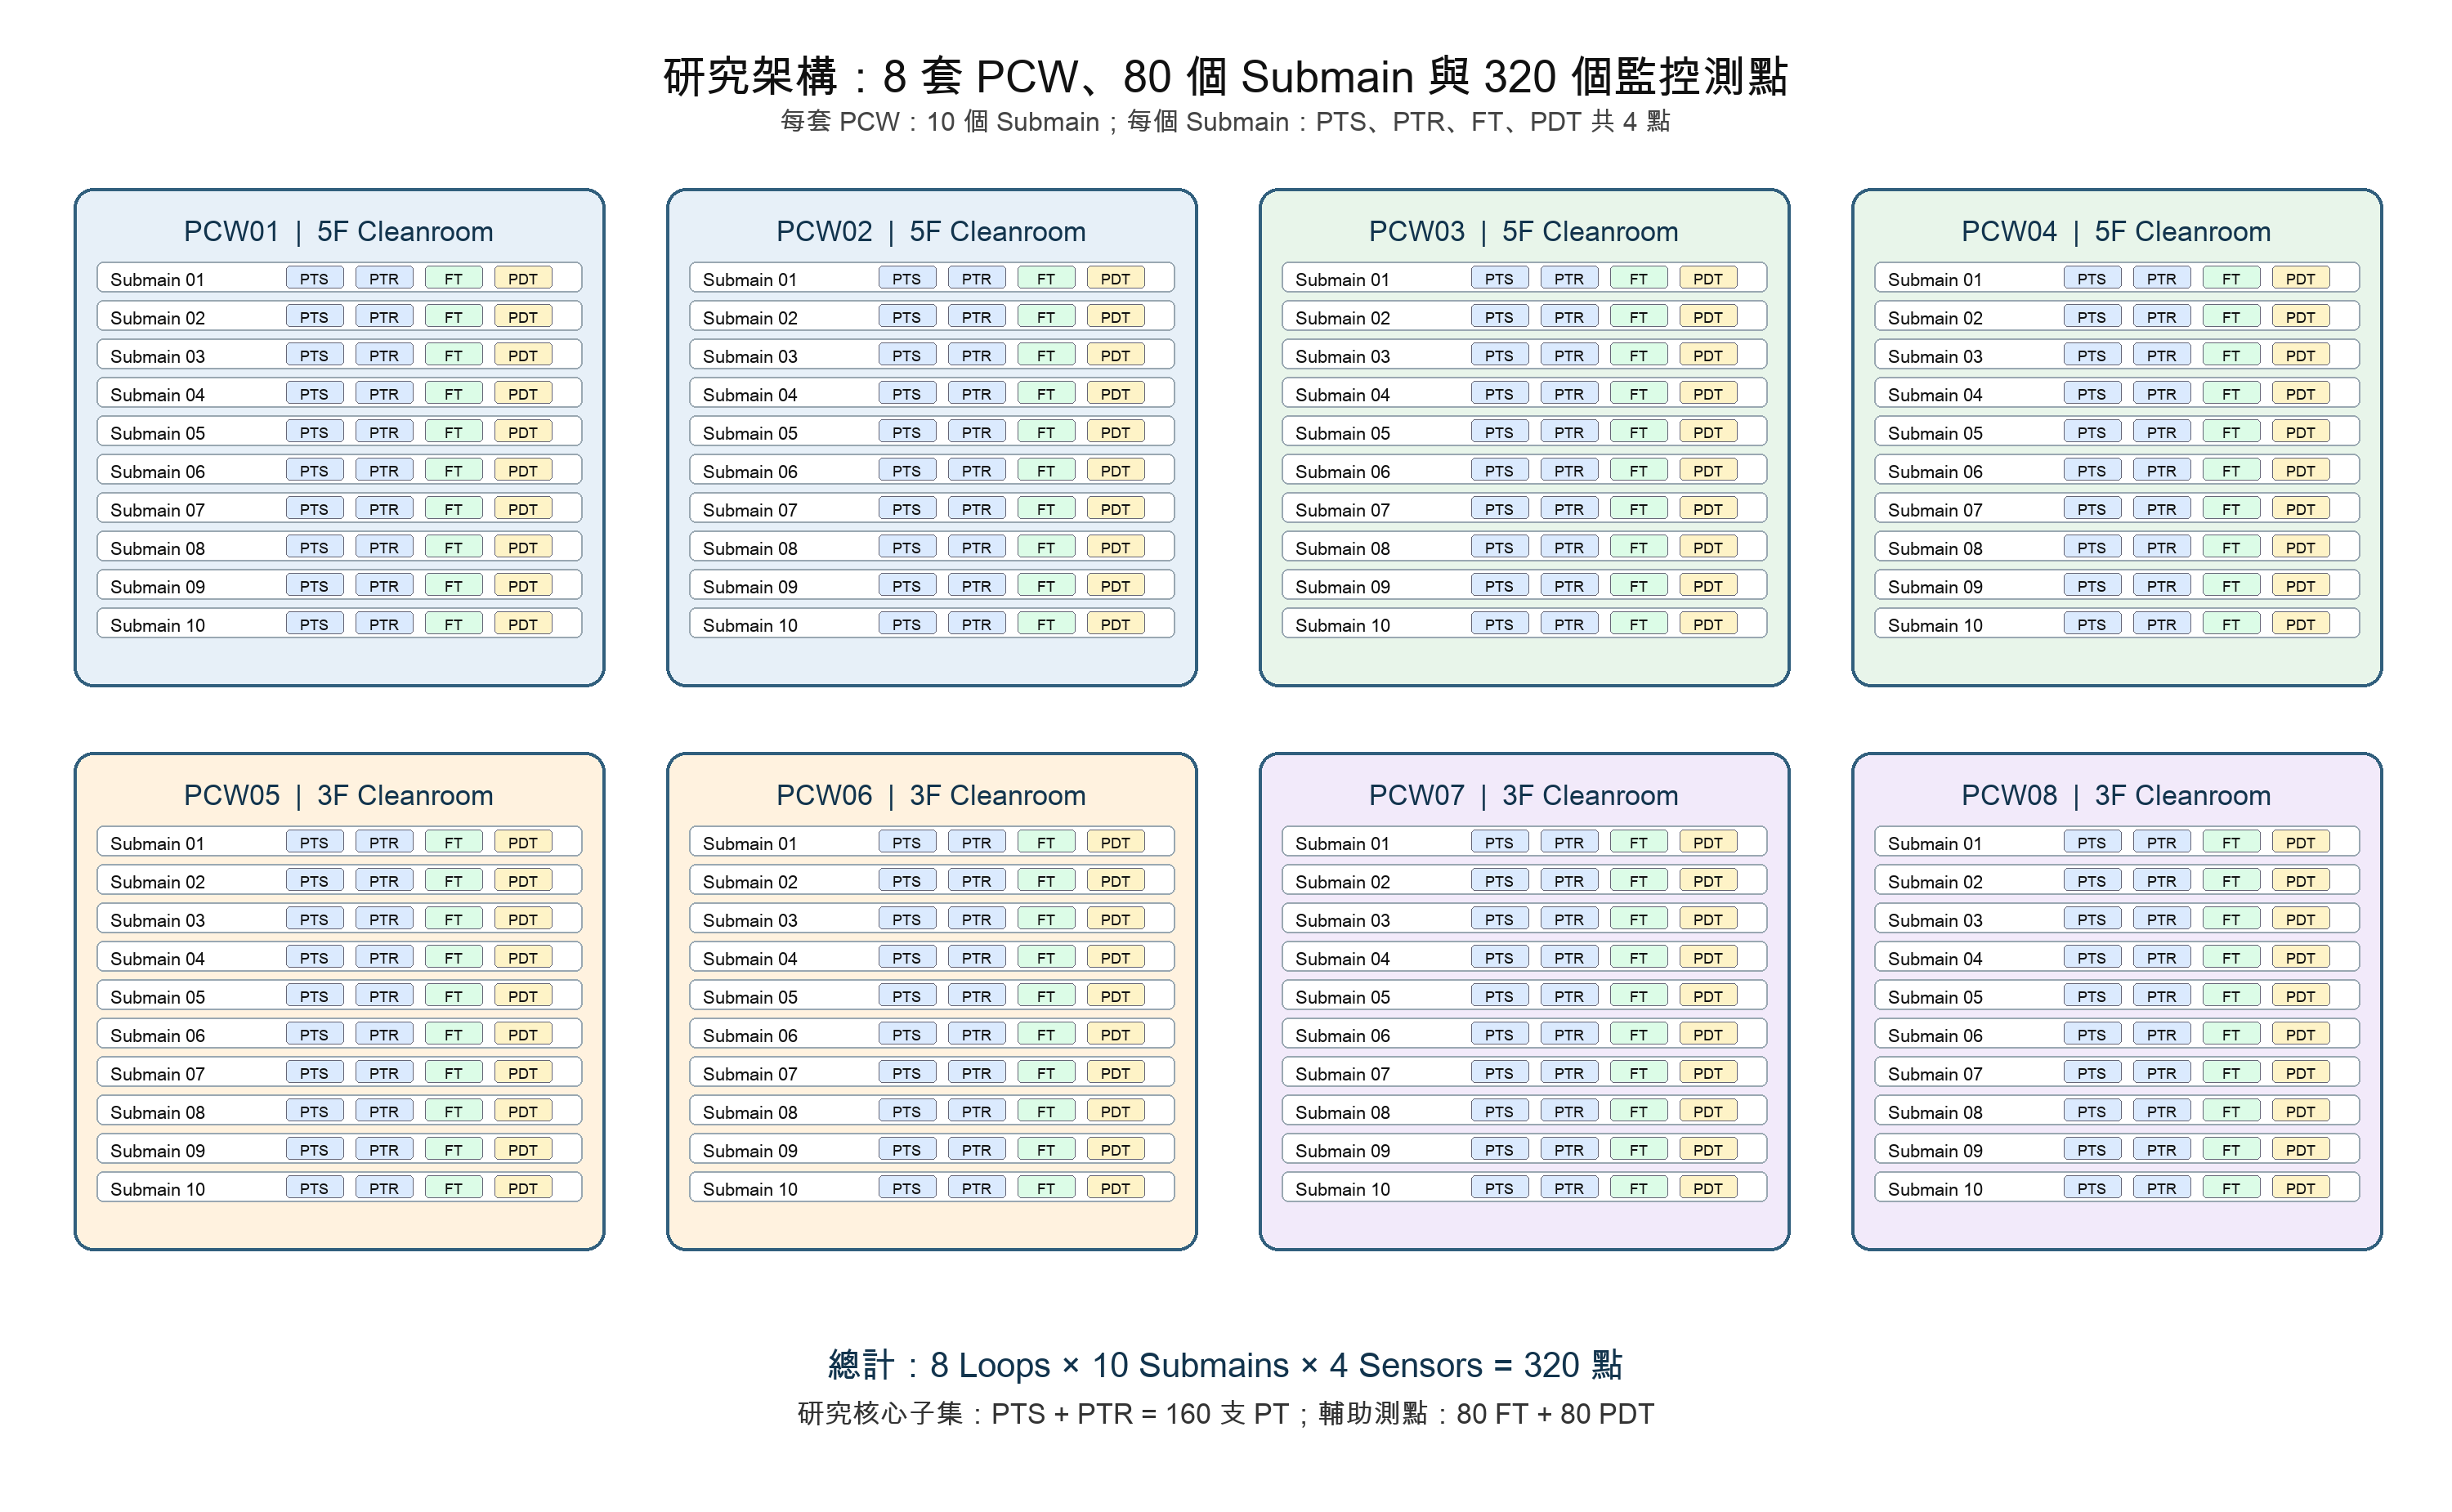
\includegraphics[width=0.95\textwidth]{picture/fig_pcw_topology_320sensors.png}
    \caption{八套 PCW、80 組 Submain 與 320 個感測器之研究拓撲層級展開圖}
    \label{fig:study_topology}
\end{figure}

\subsubsection{Sensor、PLC、SCADA 與 Historian 資料流}
本研究之系統資料流如圖 \ref{fig:data_pipeline} 所示。現場 PTS、PTR、FT 與 PDT 等感測訊號經 PLC / Remote I/O 完成工程單位縮放、時間戳記及品質碼標記後，以 Modbus TCP 提供 SCADA 讀取，資料格式採 IEEE 754 32 位元浮點數（FLOAT32 CDAB）。受限於實廠資料保密要求及產線測試條件，本研究另以 Python 之 pyModbusTCP 函式庫建置模擬伺服器，產生 8 套 PCW 系統、共 160 個壓力測點（PT-01～PT-160）與全廠 320 個監控訊號，並映射至保持暫存器（Holding Registers）40001～40320，控制介面如圖 \ref{fig:modbus_simulator_ui} 所示，映射配置如表 \ref{tab:modbus_mapping} 所示。

\begin{figure}[H]
    \centering
    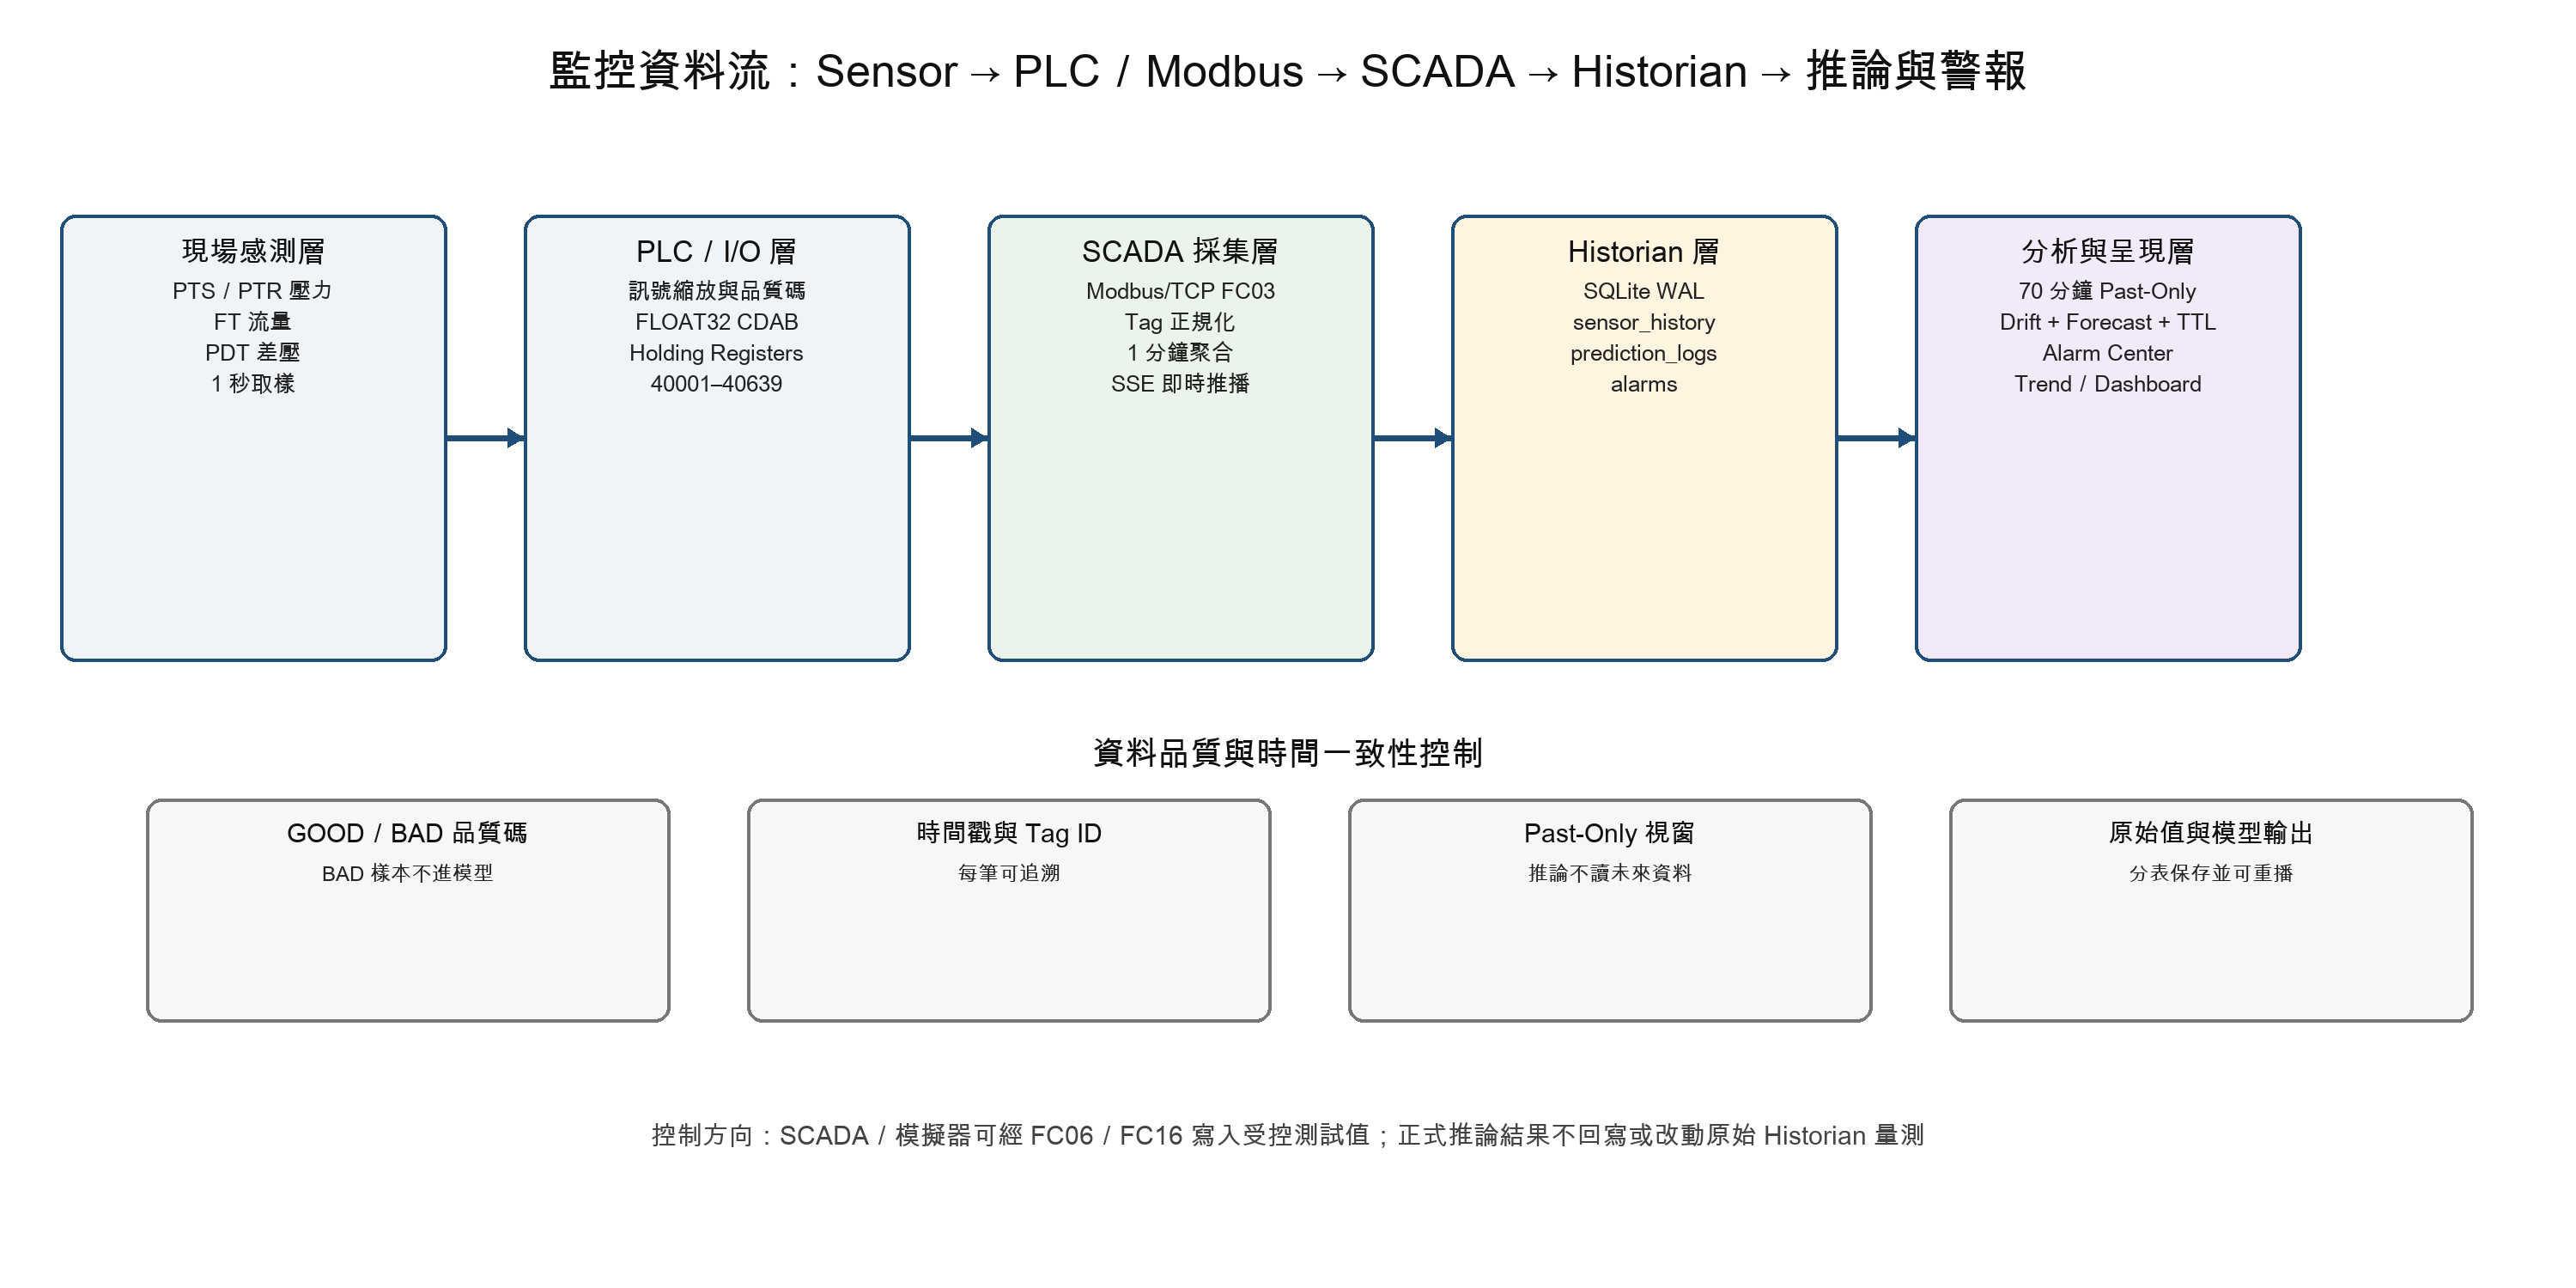
\includegraphics[width=0.95\textwidth]{picture/fig_sensor_scada_historian_flow.png}
    \caption{各類感測器經 PLC / Modbus、SCADA 至 Historian 與推論引擎之資料流向圖}
    \label{fig:data_pipeline}
\end{figure}

\begin{figure}[H]
    \centering
    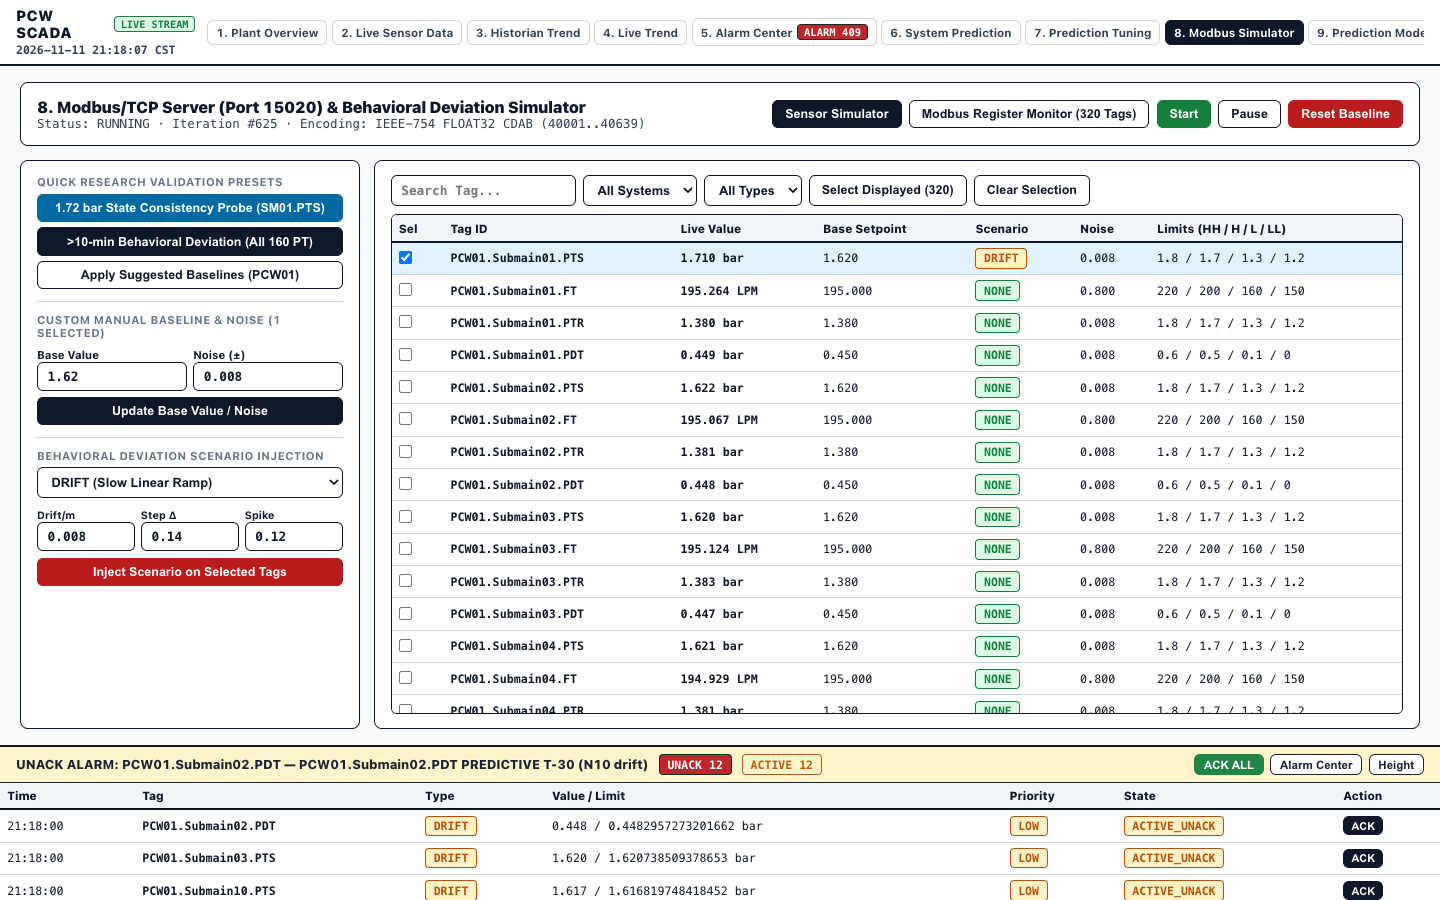
\includegraphics[width=0.90\textwidth]{picture/ui_local_modbus_simulator.png}
    \caption{Modbus TCP 伺服器訊號模擬與暫存器參數調整控制台介面}
    \label{fig:modbus_simulator_ui}
\end{figure}

\begin{table}[H]
    \centering
    \caption{全廠 320 測點 Modbus/TCP FLOAT32 保持暫存器位址映射表}
    \label{tab:modbus_mapping}
    \footnotesize
    \begin{tabularx}{\textwidth}{llccX}
        \toprule
        \textbf{暫存器位址範圍} & \textbf{資料型態} & \textbf{位元組順序} & \textbf{涵蓋測點清冊} & \textbf{工程量程與說明} \\
        \midrule
        40001--40160 & FLOAT32 (2 Regs/pt) & CDAB & PT-01 $\sim$ PT-80 (供水 PTS) & 0.00 $\sim$ 6.00 bar（各分組常態 2.50$\sim$3.50 bar） \\
        40161--40320 & FLOAT32 (2 Regs/pt) & CDAB & PT-81 $\sim$ PT-160 (回水 PTR) & 0.00 $\sim$ 5.00 bar（回水背壓 1.20$\sim$1.80 bar） \\
        40321--40480 & FLOAT32 (2 Regs/pt) & CDAB & PDT-01 $\sim$ PDT-80 (差壓) & 0.00 $\sim$ 3.00 bar（供回水壓差平衡監控） \\
        40481--40640 & FLOAT32 (2 Regs/pt) & CDAB & FT-01 $\sim$ FT-80 (流量) & 0.0 $\sim$ 500.0 LPM（次幹管流量動態負載） \\
        \bottomrule
    \end{tabularx}
\end{table}

SCADA 以每秒一次（1 Hz）的頻率擷取資料，供即時畫面顯示與警報判斷使用，並於每分鐘結束時，將該分鐘內品質碼為 GOOD 之樣本的算術平均值，寫入採用預寫式日誌（Write-Ahead Logging, WAL）模式的 SQLite 歷史資料庫（Historian）。若該分鐘 GOOD 樣本比例低於 50\%，則將該筆資料標記為 BAD 或 COMM\_LOSS，並排除於推論輸入之外。推論引擎僅讀取 Historian 中已完成分鐘彙整且符合品質條件的歷史資料，產生偏移、預測、TTL 及狀態等結果，再寫入獨立推論日誌，供監控介面查詢。模型輸出不回寫或覆蓋原始歷史值，使觀測資料、推論結果及操作紀錄得以分別追溯與稽核。

\subsubsection{核心程式與版本可追溯性}
為確保程式碼之學術誠信與工業可稽核性，如圖 \ref{fig:code_provenance} 所示，核心推論引擎原始碼清楚標示推論函式呼叫、資料品質狀態處理、預警連續確認（$K=2$）及三次解除鎖存等關鍵邏輯，並完整登記相對路徑、程式碼行號與 SHA-256 密碼學摘要，可供第三方隨時逐行比對查核。

\begin{figure}[H]
    \centering
    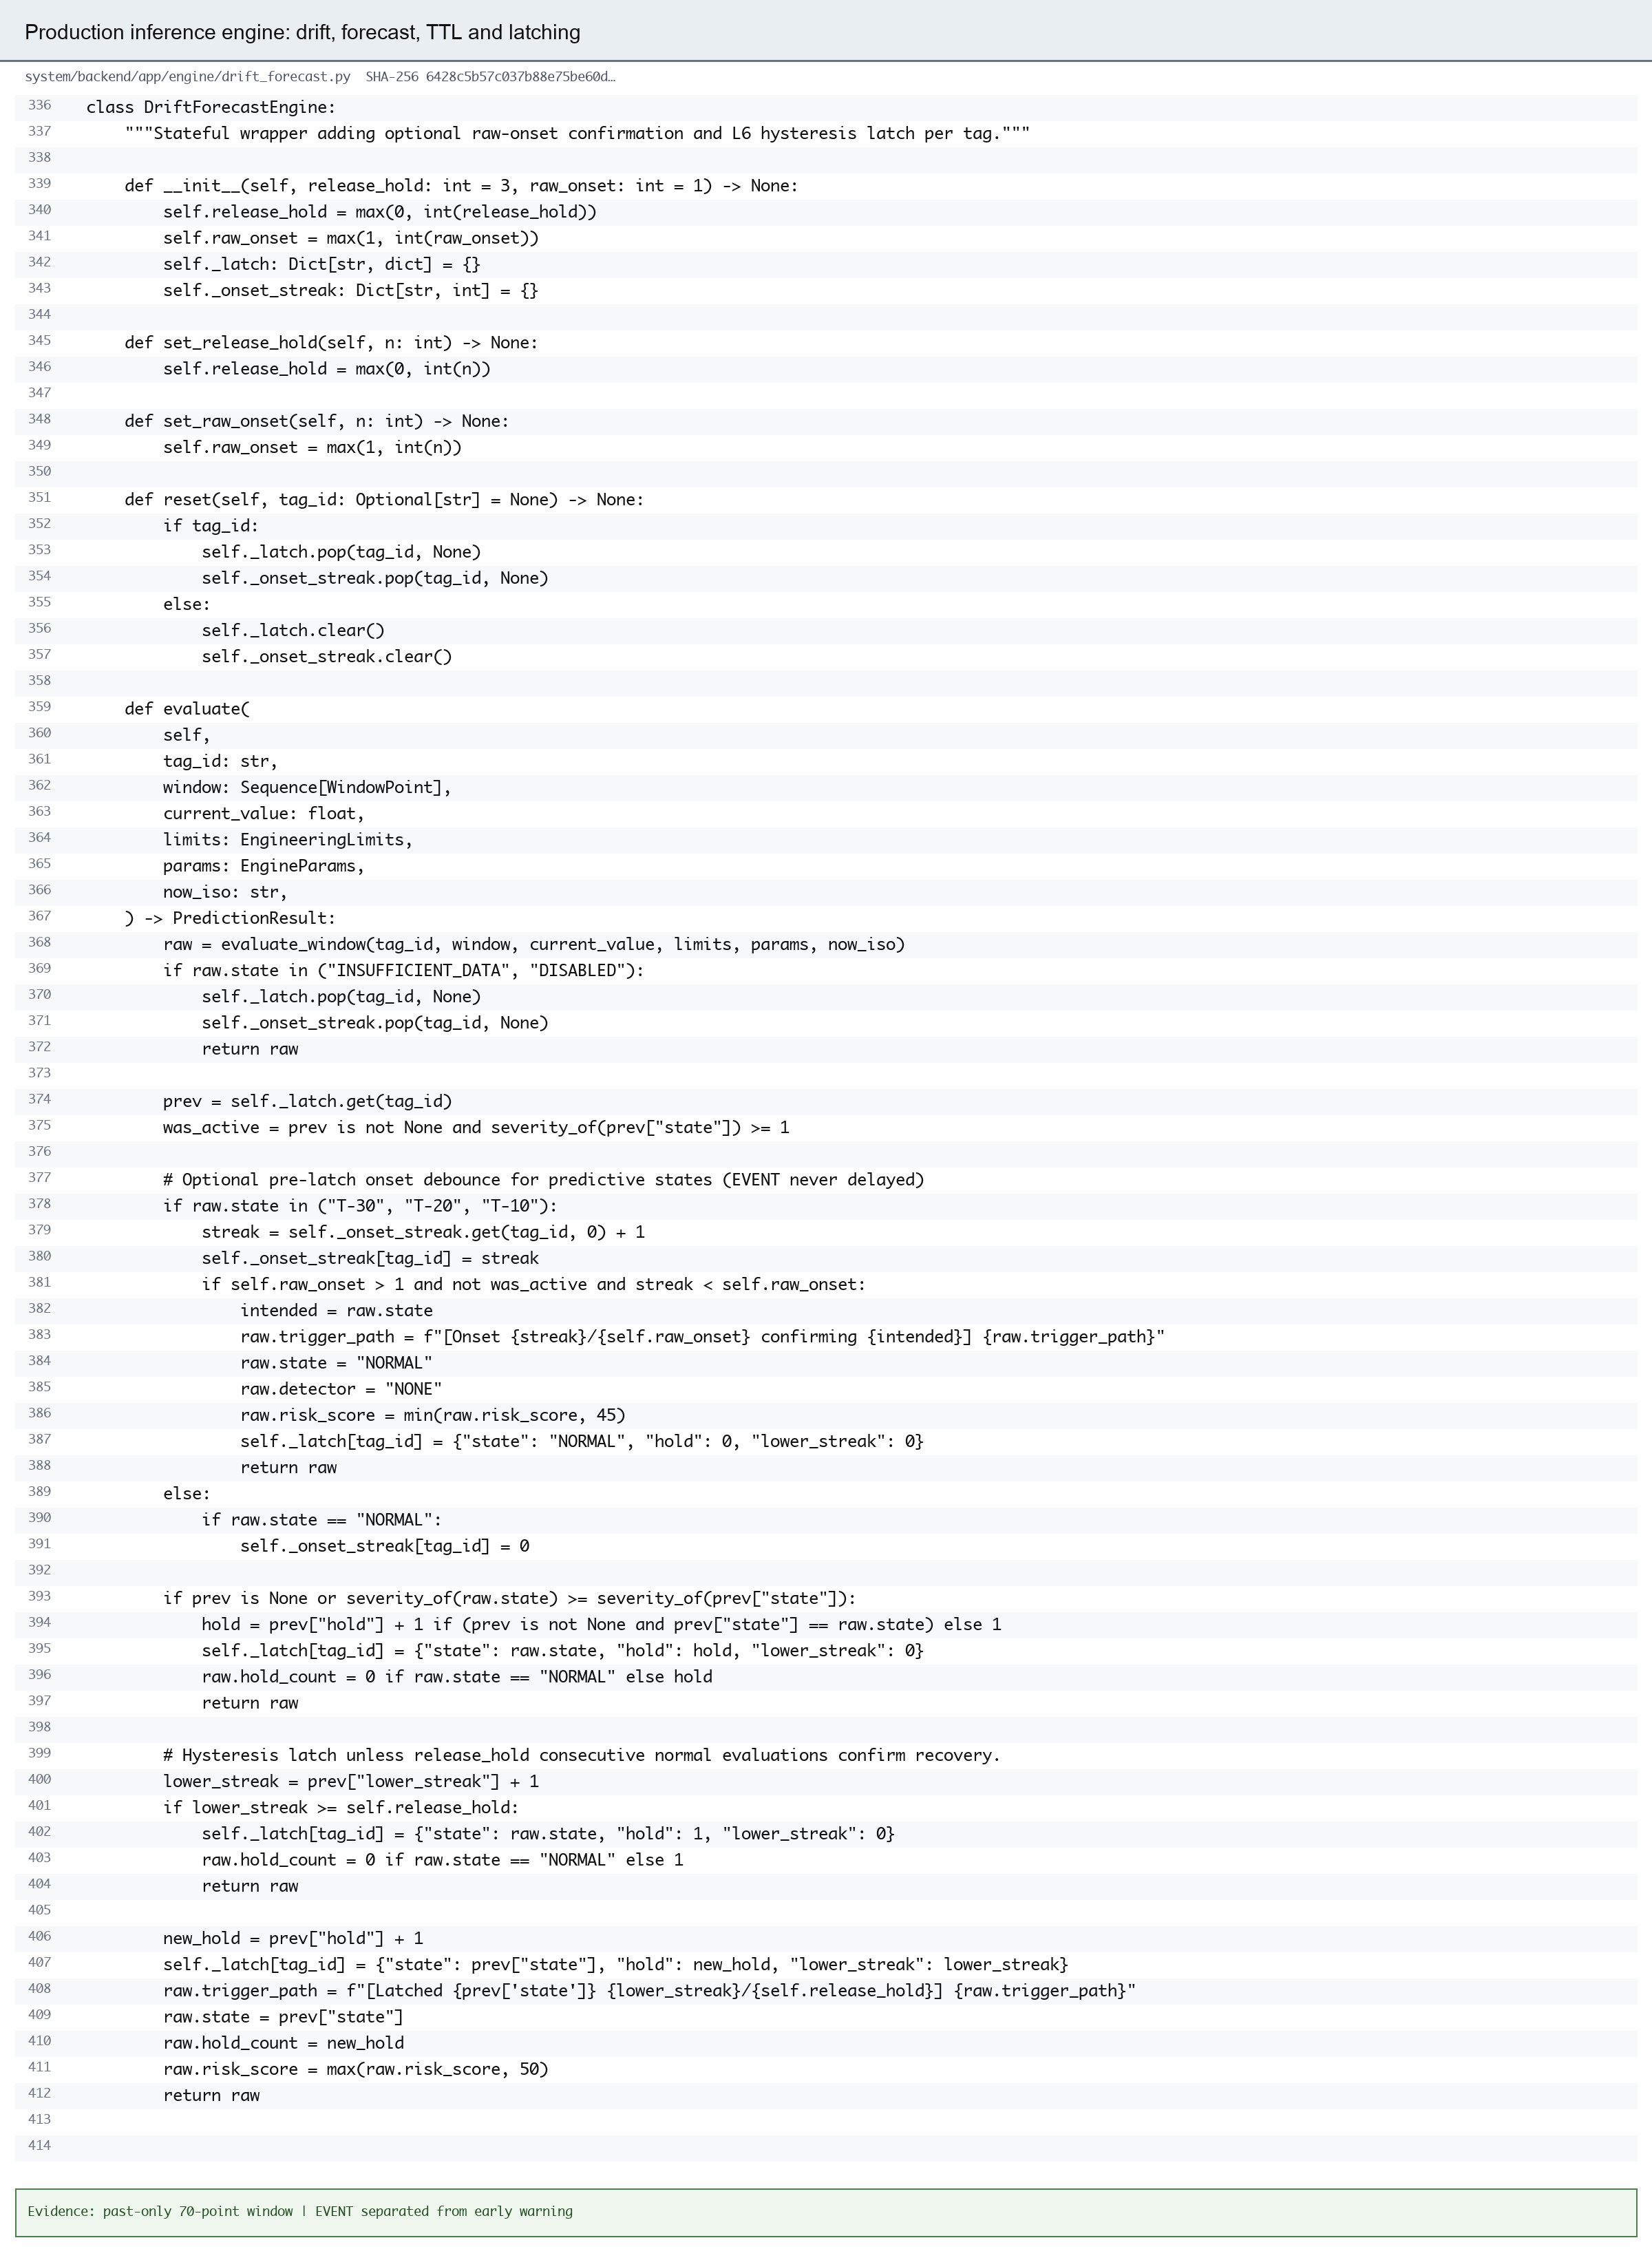
\includegraphics[width=0.85\textwidth]{picture/fig_core_inference_code_provenance.png}
    \caption{核心推論引擎實際程式碼、行號與原始檔 SHA-256 可追溯性證據截圖}
    \label{fig:code_provenance}
\end{figure}

\subsubsection{Excel 初版模型設計基礎與 Past-Only 因果滑動視窗}
本系統演算法初版以 Excel 驗證模型為設計基礎，確立了偏移偵測（Drift Detection）與趨勢預測（Trend Forecast）雙核心架構。如圖 \ref{fig:past_only_window} 所示，於任意推論時刻 $t$，系統僅讀取過去 70 分鐘已結算之觀測值，劃分為三個因果互斥區間：
\begin{enumerate}
    \item \textbf{歷史基準區間（60 分鐘）}：$B_t = [t - 70, t - 10)$，建立該測點近期之正常穩態參考值（$\text{BaseAvg}_{60}$）。
    \item \textbf{前期局部區間（5 分鐘）}：$P_t = [t - 10, t - 5)$，作為計算近期變化斜率的起始平均基準（$\text{Prev5Avg}$）。
    \item \textbf{近期局部區間（5 分鐘）}：$R_t = [t - 5, t)$，作為計算近期變化斜率的終點平均基準（$\text{Recent5Avg}$）；前後兩段 5 分鐘合併即為近期 10 分鐘觀察區間 $C_t = [t - 10, t)$。
\end{enumerate}

\begin{figure}[H]
    \centering
    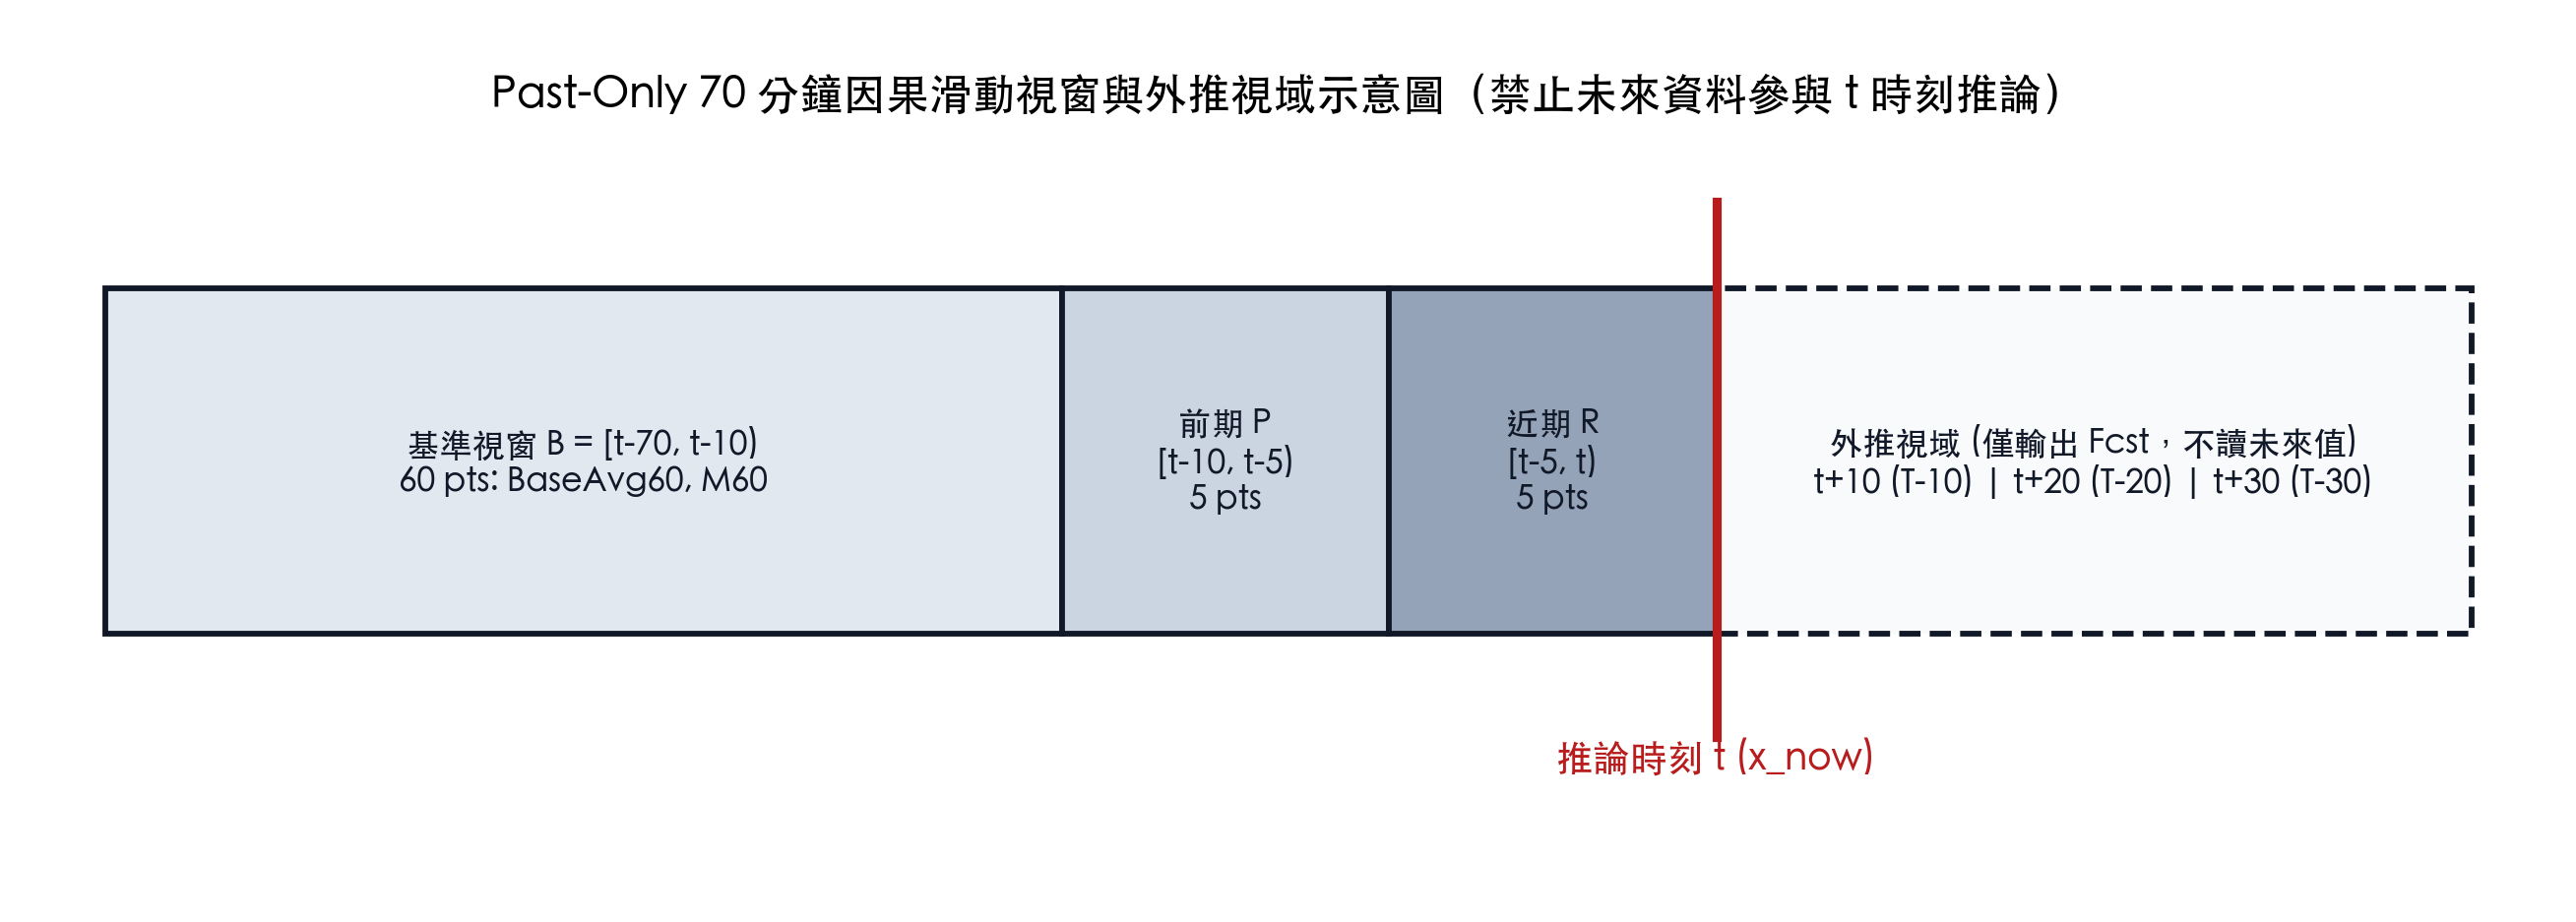
\includegraphics[width=0.95\textwidth]{picture/fig_past_only_window_design.png}
    \caption{Past-Only 70 分鐘因果滑動雙視窗（基準 60 分鐘 / 近期 10 分鐘）切分定義架構圖}
    \label{fig:past_only_window}
\end{figure}

\subsection{研究方法與推論演算法}

\subsubsection{研究範圍與輸入資料}
本研究聚焦於半導體晶圓廠 PCW 系統冷卻水壓力的早期衰退徵兆。當管壁積垢、微米濾網堵塞或二次增壓泵磨損時，水壓將脫離基準線並產生緩慢漂移。輸入資料嚴格限定為各測點過去 70 分鐘之每分鐘有效水壓觀測序列 $\{P(\tau)\}_{\tau=t-70}^{t-1}$。

\subsubsection{系統架構與推論資料流}
如圖 \ref{fig:system_layers} 所示，整體架構依工業物聯網標準自底向上整合：現場感測層 $\to$ Modbus 通訊與 Historian 快取層 $\to$ 雙核心因果推論引擎層 $\to$ SQLite WAL 持久化層 $\to$ Web SCADA 現代展示層。

\begin{figure}[H]
    \centering
    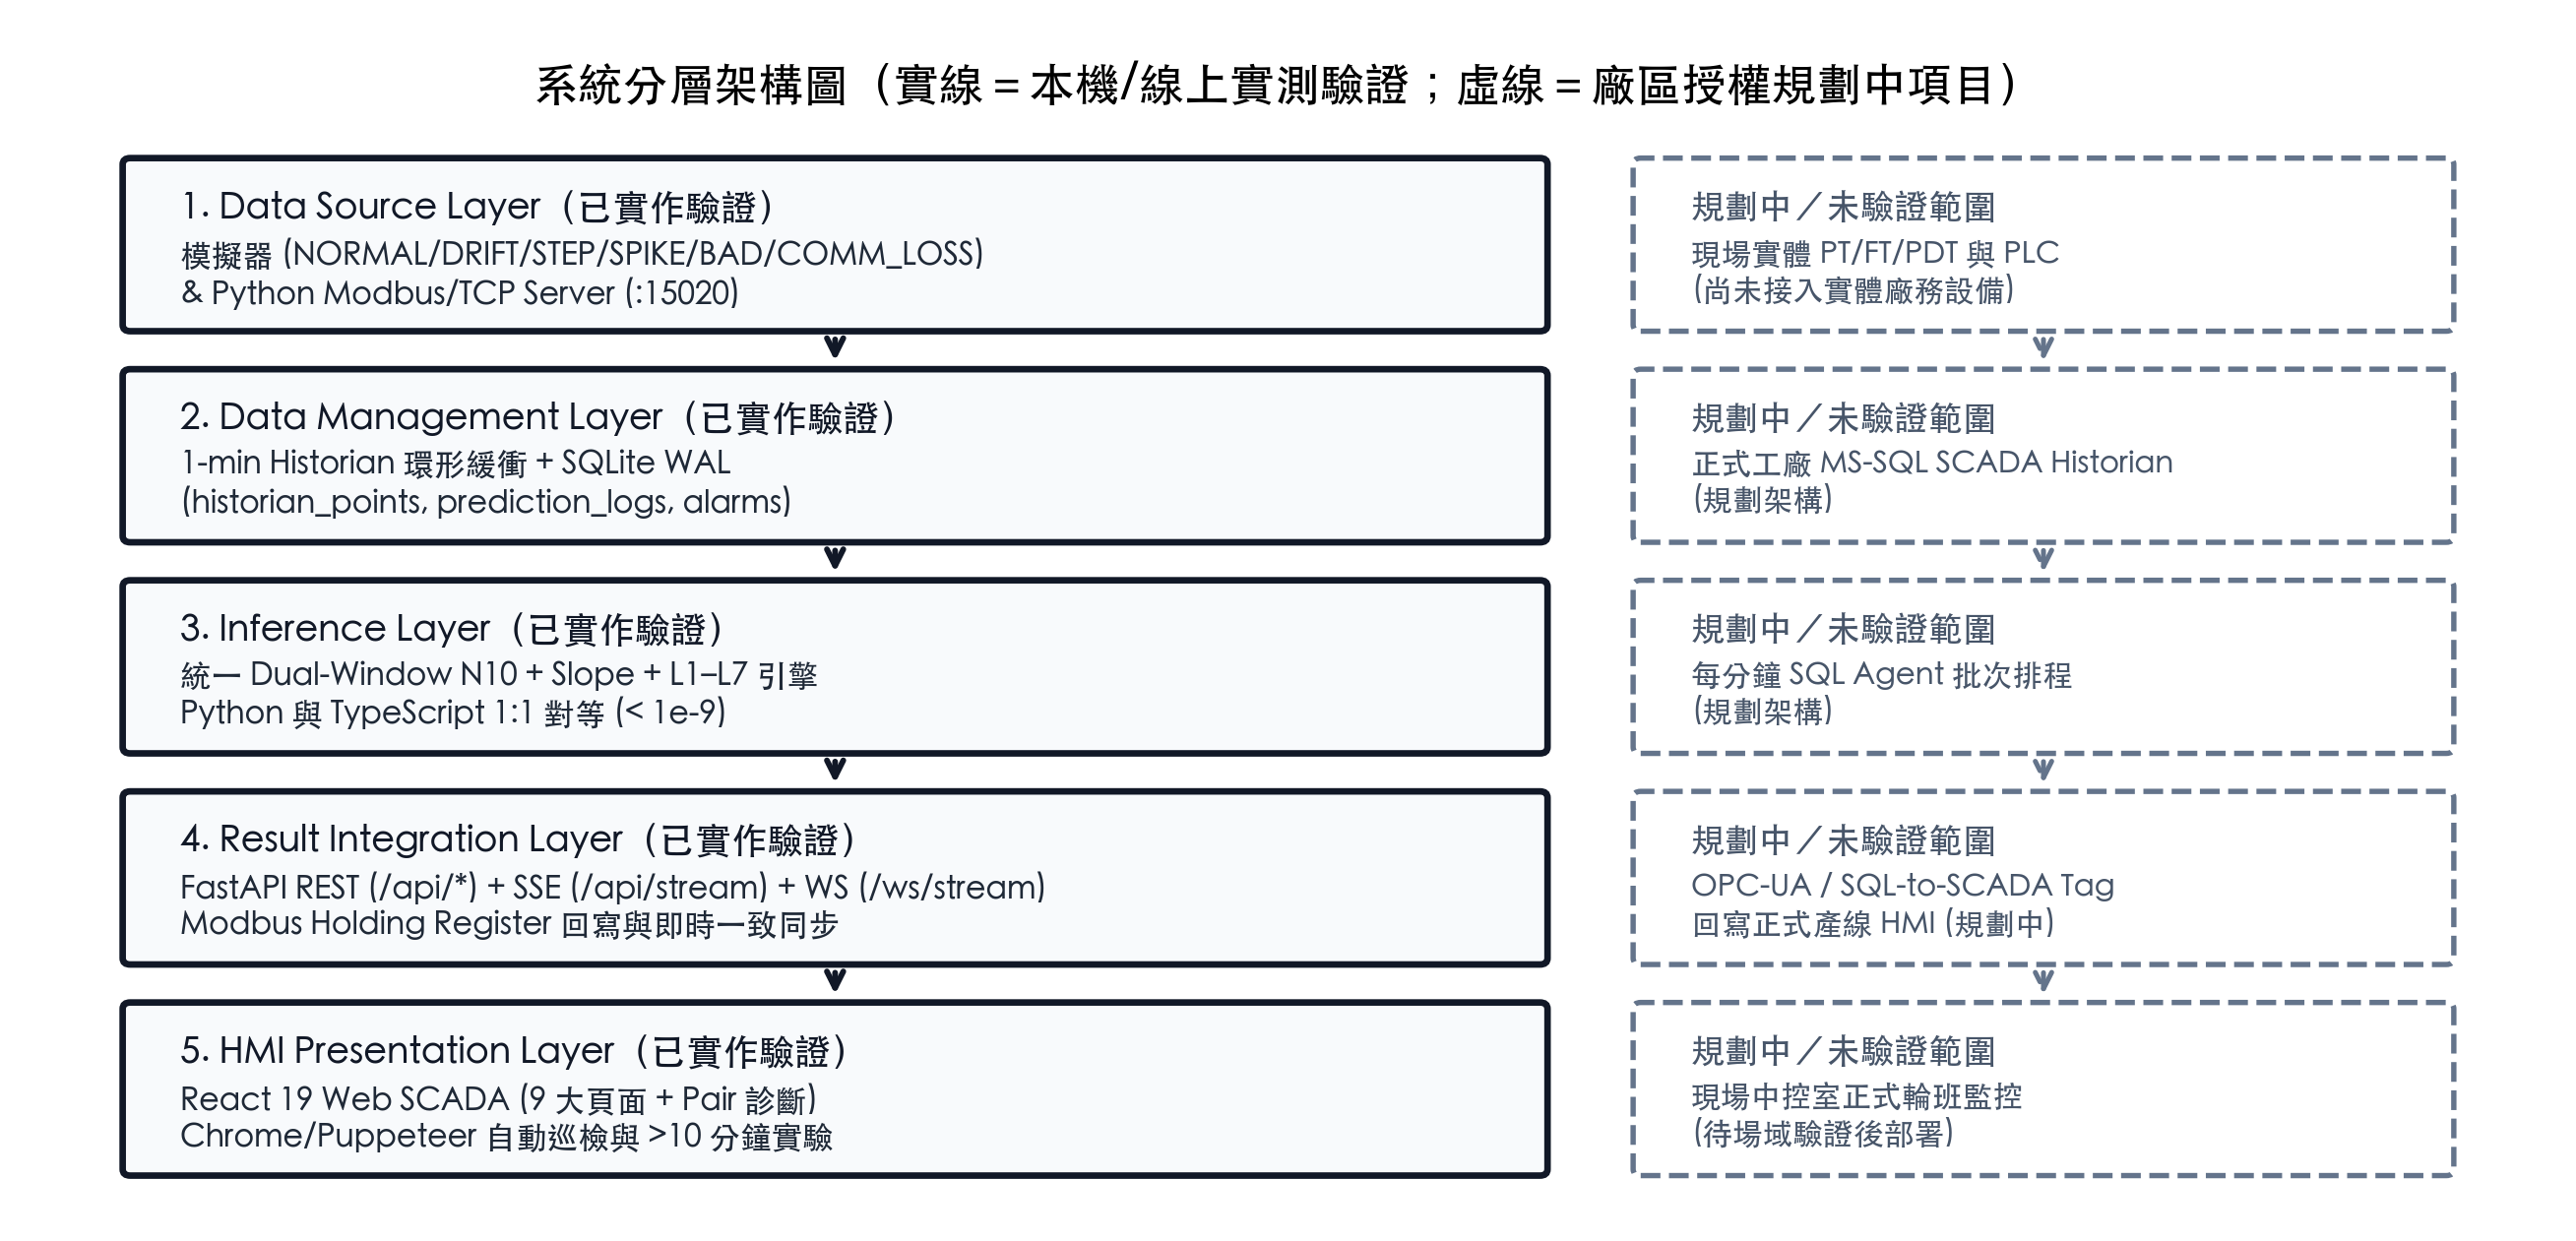
\includegraphics[width=0.95\textwidth]{picture/fig_system_architecture_layers.png}
    \caption{Web SCADA 與雙核心因果預警系統五層整合架構與資料流向拓撲圖}
    \label{fig:system_layers}
\end{figure}

\subsubsection{偏移偵測 Drift Detection}
演算法依據變化方向統計基準期與近期區間之偏離筆數：
\begin{equation}
\text{sign} = \begin{cases} +1, & \text{Recent5Avg} \ge \text{BaseAvg}_{60} \\ -1, & \text{Recent5Avg} < \text{BaseAvg}_{60} \end{cases}
\end{equation}
統計歷史基準區間 $B_t$ 內偏離超過門檻之點數 $M_{60}$，以及近期觀測區間 $C_t$ 內之偏離點數 $M_{10}$：
\begin{equation}
M_{60} = \sum_{\tau \in B_t} \mathbb{I}\left( \text{sign} \cdot [P(\tau) - \text{BaseAvg}_{60}] > g \cdot \text{BaseAvg}_{60} \right)
\end{equation}
\begin{equation}
M_{10} = \sum_{\tau \in C_t} \mathbb{I}\left( \text{sign} \cdot [P(\tau) - \text{BaseAvg}_{60}] > g \cdot \text{BaseAvg}_{60} \right)
\end{equation}
其中工程門檻比例常態設為 $g = 0.05$（5\% 偏移）。因 60 分鐘為 10 分鐘之 6 倍，常態下近期預期偏離筆數為 $M_{60}/6$。定義無因次動態偏離密度比 $N_{10}$：
\begin{equation}
N_{10} = \frac{M_{10}}{\max(1.0, M_{60} / 6.0)}
\end{equation}
同時計算滾動基線位移量 $\Delta\mu_{10} = \text{Recent5Avg} - \text{BaseAvg}_{60}$。偏移偵測成立之充分必要條件定義為：
\begin{equation}
\text{DriftDetected} = \left( N_{10} \ge \theta \right) \land \left( |\Delta\mu_{10}| \ge g \cdot \text{BaseAvg}_{60} \right)
\end{equation}
基準參數設定為 $\theta = 2.0$。此條件確保當系統發生水準位移且持續偏離時，能迅速觸發預警並防止警報早釋。

\subsubsection{趨勢預測 Forecast}
為避免單分鐘工業雜訊對數值微分造成擾動放大，演算法先計算前後兩段 5 分鐘之平滑均值，再計算單位時間斜率：
\begin{equation}
\text{Slope} = \frac{\text{Recent5Avg} - \text{Prev5Avg}}{5.0} \quad (\text{bar/min})
\end{equation}
依此斜率推導多視域外推預測值：
\begin{equation}
\hat{P}(t + h) = P(t) + \text{Slope} \cdot h, \quad h \in \{10, 20, 30\} \text{ 分鐘}
\end{equation}
為向廠務人員呈現預測不確定性，系統對近 $n = 10$ 分鐘序列擬合普通最小平方法（OLS）回歸線，在 Student-t 分佈下（自由度 8，95\% 信賴度 $t_{0.975,8} = 2.306$），推導外推 $h$ 步長之預測半寬 $\delta_h$：
\begin{equation}
\delta_h = t_{0.975, n-2} \cdot s_e \cdot \sqrt{1 + \frac{1}{n} + \frac{(t + h - \bar{\tau})^2}{\sum (\tau_i - \bar{\tau})^2}}
\end{equation}
並推導封閉解到限時間（Time-To-Limit, TTL）：
\begin{equation}
\text{TTL}(t) = \begin{cases}
\frac{P_{\text{limit}} - P(t)}{\text{Slope}}, & \text{若 } \text{Slope} \text{ 朝向安全門檻且 } |\text{Slope}| \ge 10^{-4} \\
\infty, & \text{其他平穩或背離工況}
\end{cases}
\end{equation}

\subsubsection{預警決策與工程化保護}
系統定義四階狀態機：$\text{NORMAL} \to \text{T-30} \to \text{T-20} \to \text{T-10} \to \text{EVENT}$。
\begin{enumerate}
    \item \textbf{硬事件分離（L5: Event Separation）}：若當前讀值 $P(t) \ge \text{HiHi}$ 或 $\le \text{LoLo}$，系統強制輸出最高優先級硬警報 EVENT，絕不與預警混淆。
    \item \textbf{連續兩點確認（$K=2$）}：狀態跳轉需連續兩次推論皆滿足越限條件方可確認，藉此濾除單點工業暫態毛刺。
    \item \textbf{連續三點解除鎖存（Release Hold = 3）}：當水壓回穩時，需連續 3 分鐘皆未觸發預警方解除狀態，徹底抑制門檻震盪。
\end{enumerate}

\begin{figure}[H]
    \centering
    \begin{tikzpicture}[->, >=stealth', shorten >=1pt, auto, node distance=2.8cm, semithick]
      \tikzstyle{every state}=[fill=white, draw=black, text=black, font=\small\bfseries, minimum size=1.3cm]
      \node[state] (NORMAL) {NORMAL};
      \node[state] (T30) [right of=NORMAL] {T-30};
      \node[state] (T20) [right of=T30] {T-20};
      \node[state] (T10) [right of=T20] {T-10};
      \node[state, fill=red!15] (EVENT) [right of=T10] {EVENT};

      \path 
      (NORMAL) edge [bend left=20] node [above] {\footnotesize TTL$\le$30} (T30)
      (T30) edge [bend left=20] node [above] {\footnotesize TTL$\le$20} (T20)
      (T20) edge [bend left=20] node [above] {\footnotesize TTL$\le$10} (T10)
      (T10) edge [bend left=20] node [above] {\footnotesize 越限} (EVENT)
      (T30) edge [bend left=20] node [below] {\footnotesize Hold=3} (NORMAL)
      (T20) edge [bend left=20] node [below] {\footnotesize Hold=3} (T30)
      (T10) edge [bend left=20] node [below] {\footnotesize Hold=3} (T20)
      (EVENT) edge [bend left=35] node [below] {\footnotesize 復歸} (NORMAL)
      (NORMAL) edge [bend left=40, draw=red] node [above] {\footnotesize 突發越限} (EVENT);
    \end{tikzpicture}
    \caption{四階多層預警狀態機轉移邏輯與遲滯鎖存拓撲圖}
    \label{fig:state_machine}
\end{figure}

\subsubsection{偏移偵測與趨勢預測雙路推論流程}
圖 \ref{fig:dual_path_flowchart} 將單次推論拆解為共同輸入、兩條獨立計算路徑及聯合狀態決策。共同輸入先通過 L1 品質閘門並提取 Past-Only 視窗，接著同步送入漂移偵測路徑（計算 $N_{10}$ 與 $\Delta\mu_{10}$）與趨勢預測路徑（計算均差斜率、TTL 與 OLS 95\% 信賴錐面），最終由狀態機執行階梯跳轉與鎖存。

\begin{figure}[H]
    \centering
    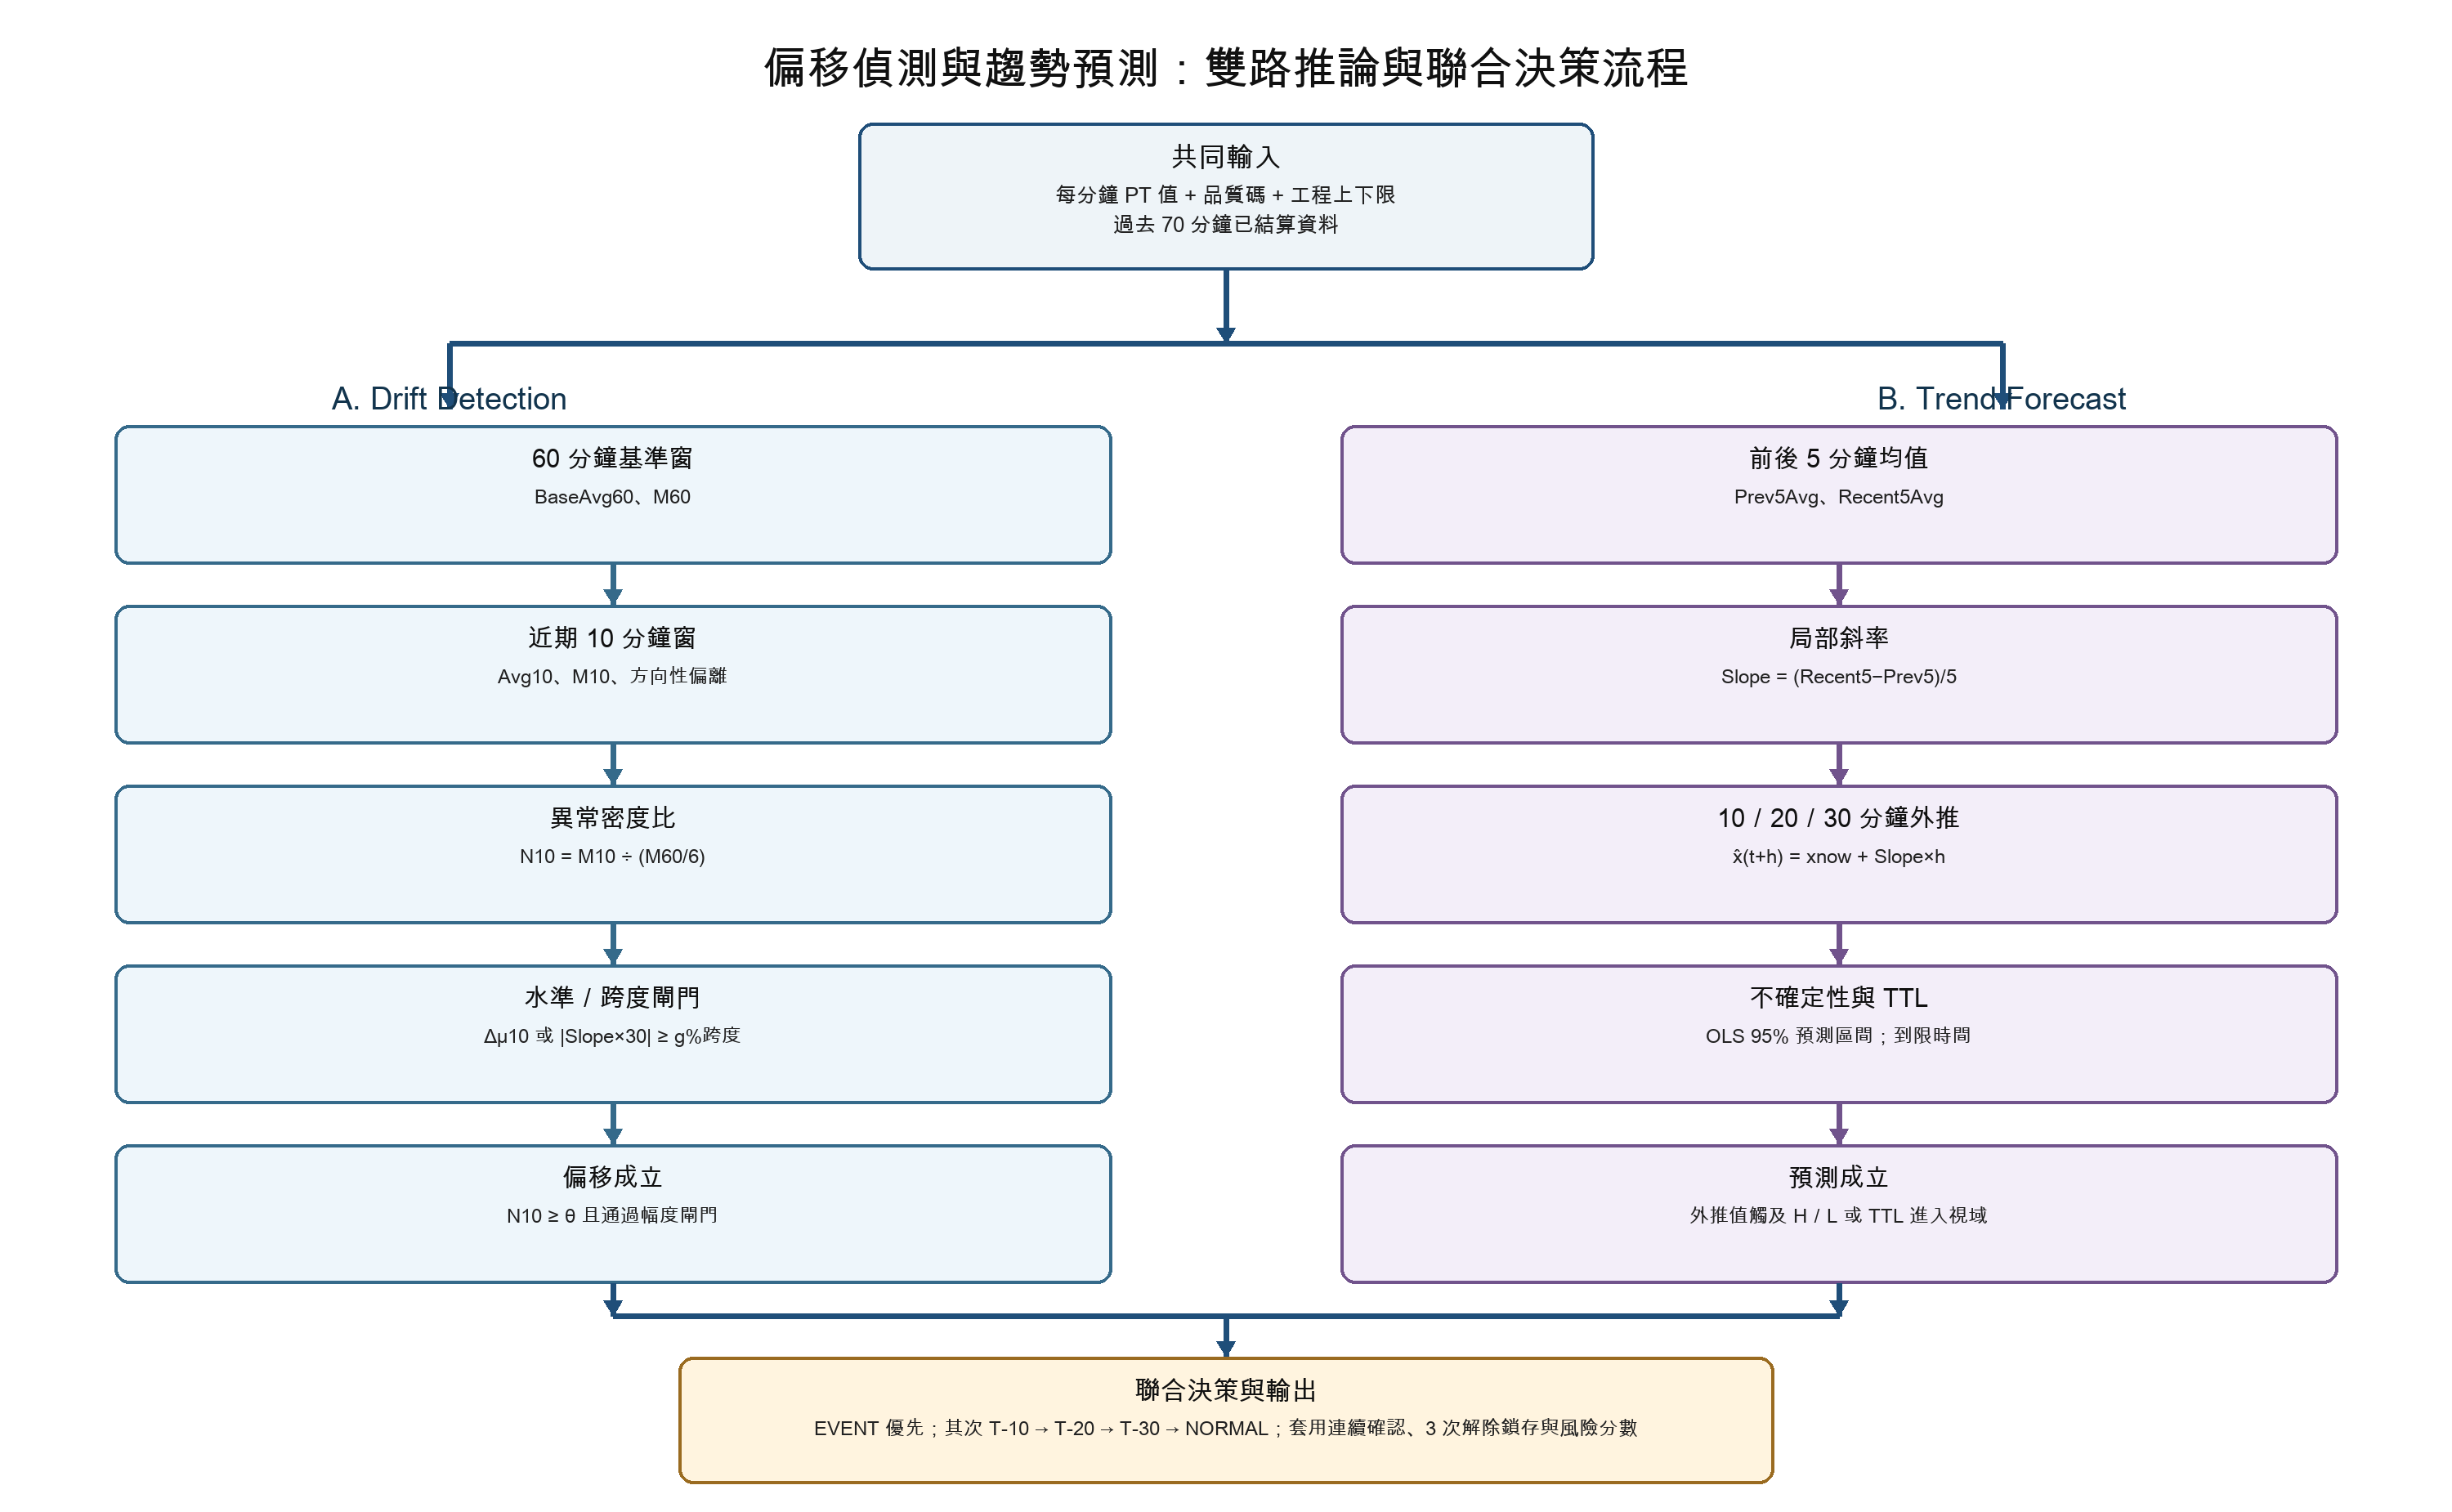
\includegraphics[width=0.95\textwidth]{picture/fig_dual_path_inference_workflow.png}
    \caption{偏移偵測與趨勢預測雙路推論、聯合判定與結果留存流程圖}
    \label{fig:dual_path_flowchart}
\end{figure}

\subsubsection{七層決策與演算法流程}
本系統整合七層防線（L1～L7），確保複雜工況下推論之確定性：
\begin{itemize}
    \item \textbf{L1 數據品質閘門}：僅計入 GOOD 樣本，近 10 分鐘有效率低於 80\% 即回傳 `INSUFFICIENT\_DATA`。
    \item \textbf{L2 雙重偏移偵測}：結合動態偏離比 $N_{10}$ 與水準位移差 $\Delta\mu_{10}$，鎖定持續性慢速漂移。
    \item \textbf{L3 不確定性量化}：OLS 95\% 預測信賴區間動態評估。
    \item \textbf{L4 剩餘時間估算}：閉式解 TTL 倒數計算。
    \item \textbf{L5 警報事件分離}：當前讀值越界時強制歸入 EVENT，不混入預警指標。
    \item \textbf{L6 前置確認與遲滯鎖存}：連續兩點確認（$K=2$），解除需連續 3 點回穩。
    \item \textbf{L7 多維風險評分}：綜合距限距離、TTL 緊迫度與偏離比輸出 $R_i \in [0, 100]$ 風險指標。
\end{itemize}

推論流程如演算法 \ref{alg:unified_inference} 所示：
\begin{algorithm}[H]
\caption{PCW 因果式雙滑動視窗漂移預測與多層狀態機聯合推論演算法}
\label{alg:unified_inference}
\begin{algorithmic}[1]
\Require 過去 70 分鐘歷史觀測值 $\{P(\tau)\}_{\tau=t-70}^{t-1}$、目前讀值 $P(t)$、安全門檻 $(P_{\text{Lo}}, P_{\text{Hi}})$、參數 $(\theta, g, K_{\text{hold}}, K)$
\Ensure 偏移指標（BaseAvg60, $N_{10}$, $\Delta\mu_{10}$）、外推預測（Slope, $\hat{P}_{t+h}$, $\delta_h$, TTL）與預警狀態 $S_t$
\State 執行 L1 數據品質檢核，若近 10 分鐘有效點數 $< 8$ 則回傳 \texttt{INSUFFICIENT\_DATA}
\State 計算歷史基準均值 BaseAvg60 與前後 5 分鐘均值 Prev5Avg, Recent5Avg
\State 計算均差斜率 $\text{Slope} = (\text{Recent5Avg} - \text{Prev5Avg}) / 5.0$
\State 統計偏離點數 $M_{60}, M_{10}$，計算動態偏離比 $N_{10}$ 與水準位移差 $\Delta\mu_{10}$
\State 評估式 (7)，判定偏移偵測標記 $\text{DriftDetected} \in \{\text{True}, \text{False}\}$
\State 計算多視域外推值 $\hat{P}_{t+h}$、OLS 95\% 信賴半寬 $\delta_h$ 與剩餘時間 TTL
\If{$P(t) \ge P_{\text{Hi}}$ \textbf{or} $P(t) \le P_{\text{Lo}}$}
    \State $S_{\text{raw}} \gets \text{EVENT}$ \Comment{L5: 硬事件分離}
\ElsIf{$\hat{P}_{t+10}$ 觸限}
    \State $S_{\text{raw}} \gets \text{T-10}$
\ElsIf{$\hat{P}_{t+20}$ 觸限}
    \State $S_{\text{raw}} \gets \text{T-20}$
\ElsIf{$\hat{P}_{t+30}$ 觸限 \textbf{or} $\text{DriftDetected} == \text{True}$}
    \State $S_{\text{raw}} \gets \text{T-30}$
\Else
    \State $S_{\text{raw}} \gets \text{NORMAL}$
\EndIf
\State 套用 L6 前置連續確認（$K=2$）與連續 3 點降級鎖存，輸出穩定狀態 $S_t$ 與風險分值 $R_t$
\end{algorithmic}
\end{algorithm}

% ==========================================
\section{實驗設計、結果分析與系統驗證}

\subsection{實驗環境、資料集性質與物理建模}

\subsubsection{實測硬體環境與資料集規格}
所有測試均在統一工業硬體平台上實施，表 \ref{tab:hardware_specs} 彙整實機探測之軟硬體規格。全廠 160 個 PT 測點實測涵蓋受控故障注入與模擬器序列，旨在驗證演算法與系統之行為正確性與即時性能。

\begin{table}[H]
    \centering
    \caption{實測硬體平台、軟體執行環境與資料集規格清冊}
    \label{tab:hardware_specs}
    \small
    \begin{tabularx}{\textwidth}{llX}
        \toprule
        \textbf{環境維度} & \textbf{實測配置項目} & \textbf{版本與規格明細} \\
        \midrule
        運算核心與記憶體 & 處理器 / RAM & Apple M5 處理器（10 核心 CPU，4P + 6E），16 GiB 高速統一記憶體 \\
        作業系統 & 系統版本 & macOS 26.7.3，Darwin Kernel Version 26.7.3 \\
        後端推論環境 & Python / 模組 & Python 3.12.14、FastAPI 0.115.0、Uvicorn 0.32.0、NumPy 1.26.4 \\
        資料庫引擎 & SQLite WAL & SQLite 3.43.2，啟用 Write-Ahead Logging (WAL) 與同步快取模式 \\
        前端展示技術棧 & 前端框架 / 瀏覽器 & Node.js v24.14.1、React 19.2.8、Vite 8.3.0、Google Chrome 157.0.8103.40 \\
        驗證資料集規模 & 實驗場次清冊 & 160 PT $\times$ 12 情境 = 1,920 場固定種子受控試驗（Seed = 20261111） \\
        歷史基準資料集 & 基準工作簿 & Excel 基準工作簿（\texttt{PT-1} 測點，480 分鐘連續工業遙測序列） \\
        \bottomrule
    \end{tabularx}
\end{table}

\subsubsection{基準 Excel 驗證模型之工作表功能拓撲}
為確保演算法具備高度的可重現性與工業權威性，本研究以指導教授審定之標準基準工作簿（\texttt{PCW\_T30\_T20\_T10\_FINAL\_ROLLBACK\_THESIS\_VERIFICATION.xlsx}）作為數值黃金標準（Ground Truth）。該工作簿深入封裝了 10 大核心功能工作表，各工作表職掌與因果特性如表 \ref{tab:excel_sheets} 所示。

\begin{table}[H]
    \centering
    \caption{Excel 基準驗證工作簿（10 大功能工作表）結構清冊與用途說明}
    \label{tab:excel_sheets}
    \footnotesize
    \begin{tabularx}{\textwidth}{llccl}
        \toprule
        \textbf{工作表名稱} & \textbf{功能定位與核心職掌} & \textbf{紀錄筆數} & \textbf{更新頻率} & \textbf{因果安全防線} \\
        \midrule
        \texttt{Parameters} & 系統全域工程參數與門檻定義表 & 8 項全域常數 & 靜態配置 & 嚴禁動態篡改，推論時鎖定 \\
        \texttt{RawData} & 實廠壓力感測器原始分秒採樣時序記錄 & 480 筆連續序列 & 逐分鐘記錄 & 嚴格物理採樣，保留雜訊毛刺 \\
        \texttt{MinuteInference} & 雙視窗滑動計算與 24 欄位逐分推論引擎 & 480 筆（A$\sim$X 欄） & 逐分鐘串流 & 過去視窗計算，禁止向後引用 \\
        \texttt{Model\_Logic} & 線上即時推論與離線驗證標籤規則表 & 邏輯定義規格 & 靜態規則 & 劃分即時推論與離線評估界限 \\
        \texttt{Alarm\_Engine} & 四階狀態機跳轉與雙向鎖存消抖邏輯表 & 480 筆狀態履歷 & 事件驅動 & 連續 2 點確認，連續 3 點解鎖 \\
        \texttt{LeadTime\_Stats} & 預警提前量（Lead Time）與到限時間統計 & 統計摘要分析 & 批次計算 & 事後驗證標籤，評定處置窗口 \\
        \texttt{Data\_Quality} & 採樣完整率、缺值插補與無效碼過濾表 & 480 筆品質代碼 & 逐分鐘檢核 & 有效率過半表決，剔除 BAD 碼 \\
        \texttt{Confusion\_Matrix} & TP / FP / TN / FN 矩陣與 F1 指標核算表 & 評估矩陣清冊 & 實驗結算 & 依離線真實越限標籤交叉結算 \\
        \texttt{SCADA\_Mapping} & Modbus TCP 保持暫存器地址與工程換算表 & 320 測點映射 & 協定配置 & 定義 FLOAT32 CDAB 位址空間 \\
        \texttt{Thesis\_Model} & 論文數學模型之封閉解對齊工作表 & 480 筆 & 模型比對 & 驗證跨平台吻合度（誤差 0.0） \\
        \bottomrule
    \end{tabularx}
\end{table}

\texttt{Parameters} 工作表記載 8 大核心工程參數，如表 \ref{tab:excel_parameters} 所示。
\begin{table}[H]
    \centering
    \caption{\texttt{Parameters} 工作表 8 大核心參數設定清冊}
    \label{tab:excel_parameters}
    \small
    \begin{tabularx}{\textwidth}{llccl}
        \toprule
        \textbf{參數變數名稱} & \textbf{物理意義與工程功能} & \textbf{基準設定值} & \textbf{工程單位} & \textbf{設計依據與保護目的} \\
        \midrule
        \texttt{BaseWindow} & 歷史基準滾動滑動視窗長度 & 60 & 分鐘 (min) & 建立長期穩態水準，抑制單元工況波動 \\
        \texttt{RecentWindow} & 近期局部觀測滑動視窗長度 & 10 & 分鐘 (min) & 捕捉當前水力阻抗變化趨勢 \\
        \texttt{SubWindow} & 前期/近期均差分析子視窗長度 & 5 & 分鐘 (min) & 濾除高頻脈衝，提供穩健微分基準 \\
        \texttt{Threshold\_g} & 顯著偏離動態比例門檻 & 0.05 (5\%) & 無因次比率 & 判定水壓偏離基準值之顯著性界限 \\
        \texttt{Density\_Theta} & 異常事件密度增長倍比門檻 & 2.0 & 倍數比率 & 抑制管網高斯白雜訊引發之虛警 \\
        \texttt{LeadTime\_Horizon} & 多階梯早期預警最大預測視域 & 30 & 分鐘 (min) & 提供廠務人員充足之黃金應變處置窗口 \\
        \texttt{Confirm\_Count} & 預警狀態觸發前置連續確認點數 & 2 & 連續採樣點 & 徹底濾除單點暫態毛刺干擾 \\
        \texttt{Hold\_Count} & 預警降級或解除所需連續平穩點數 & 3 & 連續採樣點 & 消除門檻邊界頻繁跳躍（Chattering） \\
        \bottomrule
    \end{tabularx}
\end{table}

\texttt{MinuteInference} 工作表展開 24 個標準欄位（A～X 欄），依功能區分為兩大子表：表 \ref{tab:minute_inference_pt1} 涵蓋觀測與因果特徵（A～L 欄），表 \ref{tab:minute_inference_pt2} 涵蓋推論狀態與離線驗證（M～X 欄）。

\begin{table}[H]
    \centering
    \caption{\texttt{MinuteInference} 工作表欄位清冊（第一部分：A～L 欄 觀測與因果特徵）}
    \label{tab:minute_inference_pt1}
    \footnotesize
    \begin{tabularx}{\textwidth}{llccX}
        \toprule
        \textbf{欄位代號} & \textbf{欄位名稱} & \textbf{資料型態} & \textbf{計算視域} & \textbf{運算公式與定義} \\
        \midrule
        Col A & \texttt{Timestamp} & 字串/時間 & 當前 $t$ & ISO-8601 分鐘時間戳記 \\
        Col B & \texttt{Pressure\_Now} & 浮點數 (bar) & 當前 $t$ & 現場感測器當前分鐘平均水壓值 $P(t)$ \\
        Col C & \texttt{Quality\_Code} & 字串代碼 & $[t-1, t)$ & 數據品質代碼（GOOD, BAD, COMM\_LOSS） \\
        Col D & \texttt{BaseAvg60} & 浮點數 (bar) & $[t-70, t-10)$ & 過去 60 分鐘歷史基準區間平均值 \\
        Col E & \texttt{Prev5Avg} & 浮點數 (bar) & $[t-10, t-5)$ & 前期 5 分鐘均差起始基準值 \\
        Col F & \texttt{Recent5Avg} & 浮點數 (bar) & $[t-5, t)$ & 近期 5 分鐘均差終點基準值 \\
        Col G & \texttt{Slope\_5m} & 浮點數 (bar/min) & $[t-10, t)$ & 單位時間均差斜率 $(\text{Recent5Avg}-\text{Prev5Avg})/5$ \\
        Col H & \texttt{M60\_Count} & 整數點數 & $[t-70, t-10)$ & 基準窗 60 分鐘內偏離超過 5\% 之點數 \\
        Col I & \texttt{M10\_Count} & 整數點數 & $[t-10, t)$ & 近期窗 10 分鐘內偏離超過 5\% 之點數 \\
        Col J & \texttt{N10\_Ratio} & 浮點數倍比 & 複合計算 & 動態偏離事件密度比 $M_{10} / \max(1.0, M_{60}/6)$ \\
        Col K & \texttt{Delta\_Mu} & 浮點數 (bar) & 複合計算 & 滾動基線位移量 $\text{Recent5Avg} - \text{BaseAvg60}$ \\
        Col L & \texttt{Drift\_Flag} & 布林旗標 & 當前 $t$ & 漂移判定：$(N_{10} \ge 2.0) \land (|\Delta\mu| \ge 0.05 \times \text{BaseAvg})$ \\
        \bottomrule
    \end{tabularx}
\end{table}

\begin{table}[H]
    \centering
    \caption{\texttt{MinuteInference} 工作表欄位清冊（第二部分：M～X 欄 推論狀態與離線驗證）}
    \label{tab:minute_inference_pt2}
    \footnotesize
    \begin{tabularx}{\textwidth}{llccX}
        \toprule
        \textbf{欄位代號} & \textbf{欄位名稱} & \textbf{資料型態} & \textbf{計算視域} & \textbf{運算公式與定義} \\
        \midrule
        Col M & \texttt{Pred\_P10} & 浮點數 (bar) & 外推 10 分鐘 & 未來 10 分鐘線性外推預測值 $P(t) + 10 \times \text{Slope}$ \\
        Col N & \texttt{Pred\_P20} & 浮點數 (bar) & 外推 20 分鐘 & 未來 20 分鐘線性外推預測值 $P(t) + 20 \times \text{Slope}$ \\
        Col O & \texttt{Pred\_P30} & 浮點數 (bar) & 外推 30 分鐘 & 未來 30 分鐘線性外推預測值 $P(t) + 30 \times \text{Slope}$ \\
        Col P & \texttt{OLS\_Slope} & 浮點數 (bar/min) & $[t-10, t)$ & 近 10 點普通最小平方法回歸斜率 \\
        Col Q & \texttt{OLS\_CI95\_Half} & 浮點數 (bar) & 外推視域 & Student-t 95\% 預測信賴區間半寬 $\delta_h$ \\
        Col R & \texttt{TTL\_Minutes} & 浮點數 (min) & 封閉外推 & 距目標安全門檻之預測剩餘到限時間 \\
        Col S & \texttt{Raw\_State} & 狀態代碼 & 當前瞬時 & 瞬時未確認狀態機輸出（NORMAL, T-30, T-20, T-10, EVENT） \\
        Col T & \texttt{Confirmed\_State} & 狀態代碼 & 連續確認 & 經連續 2 點確認與 3 點解鎖之最終發布狀態 \\
        Col U & \texttt{GroundTruth\_Event} & 布林標籤 & $[t, t+30]$ (離線) & 未來 30 分鐘內是否實際越過安全門檻之真值標籤 \\
        Col V & \texttt{LeadTime\_Actual} & 浮點數 (min) & 事後結算 (離線) & 自首次確認預警至實際越限之真實處置時間 \\
        Col W & \texttt{Evaluation\_Class} & 類別標籤 & 統計結算 (離線) & 混淆矩陣分類（TP, FP, TN, FN） \\
        Col X & \texttt{Audit\_SHA256} & 雜湊字串 & 全行加密 & 本列 23 欄位數據之 SHA-256 密碼學檢驗碼 \\
        \bottomrule
    \end{tabularx}
\end{table}

\subsubsection{實驗程序、原始輸出與證據}
實驗矩陣程式如圖 \ref{fig:experiment_matrix_code} 所示：每一測點依序產生 8 種異常與 4 種非異常/干擾情境（共 12 種情境，如表 \ref{tab:experiment_scenarios} 所示）；同一輸入序列同時送入 Static、EWMA、Naive OLS 與本研究所提架構，徹底杜絕不同模型使用不同資料造成的評測偏差。執行終端摘要與 SHA-256 如圖 \ref{fig:terminal_sha256_evidence} 所示。

\begin{figure}[H]
    \centering
    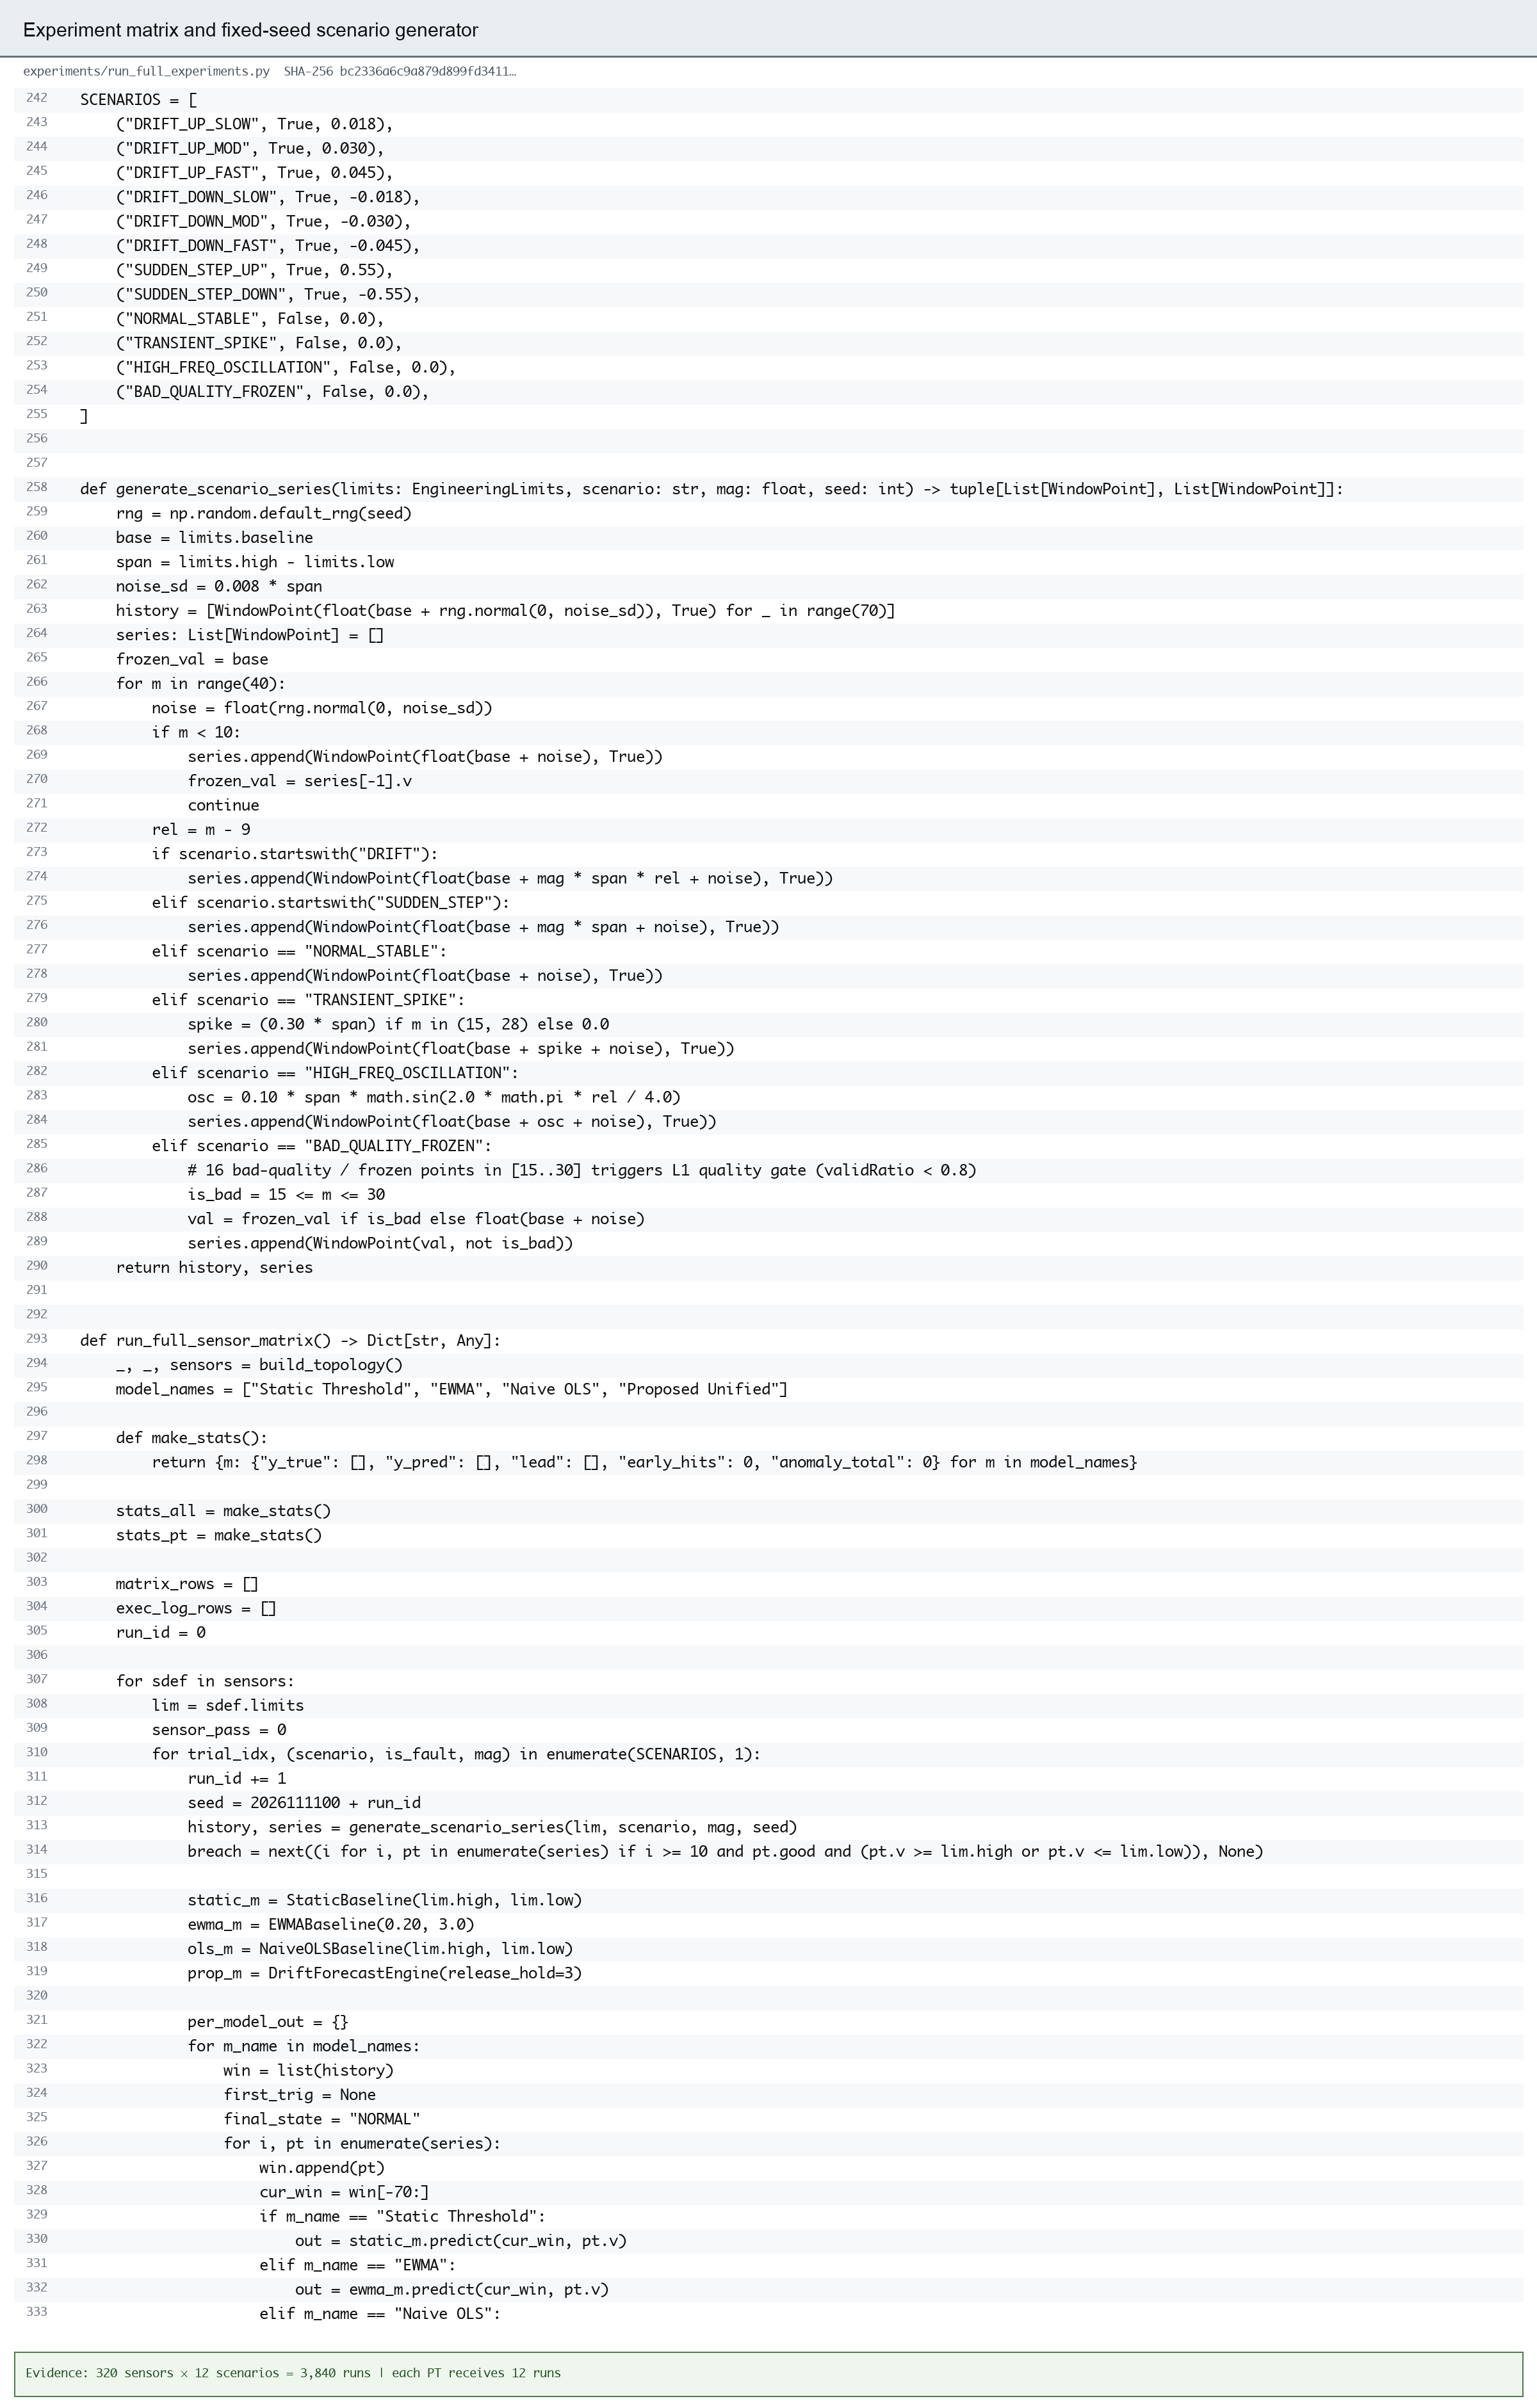
\includegraphics[width=0.88\textwidth]{picture/fig_experiment_matrix_code_1920.png}
    \caption{全廠 160PT、1,920 場試驗矩陣、固定種子情境產生器與多模型公平比較程式碼}
    \label{fig:experiment_matrix_code}
\end{figure}

\begin{figure}[H]
    \centering
    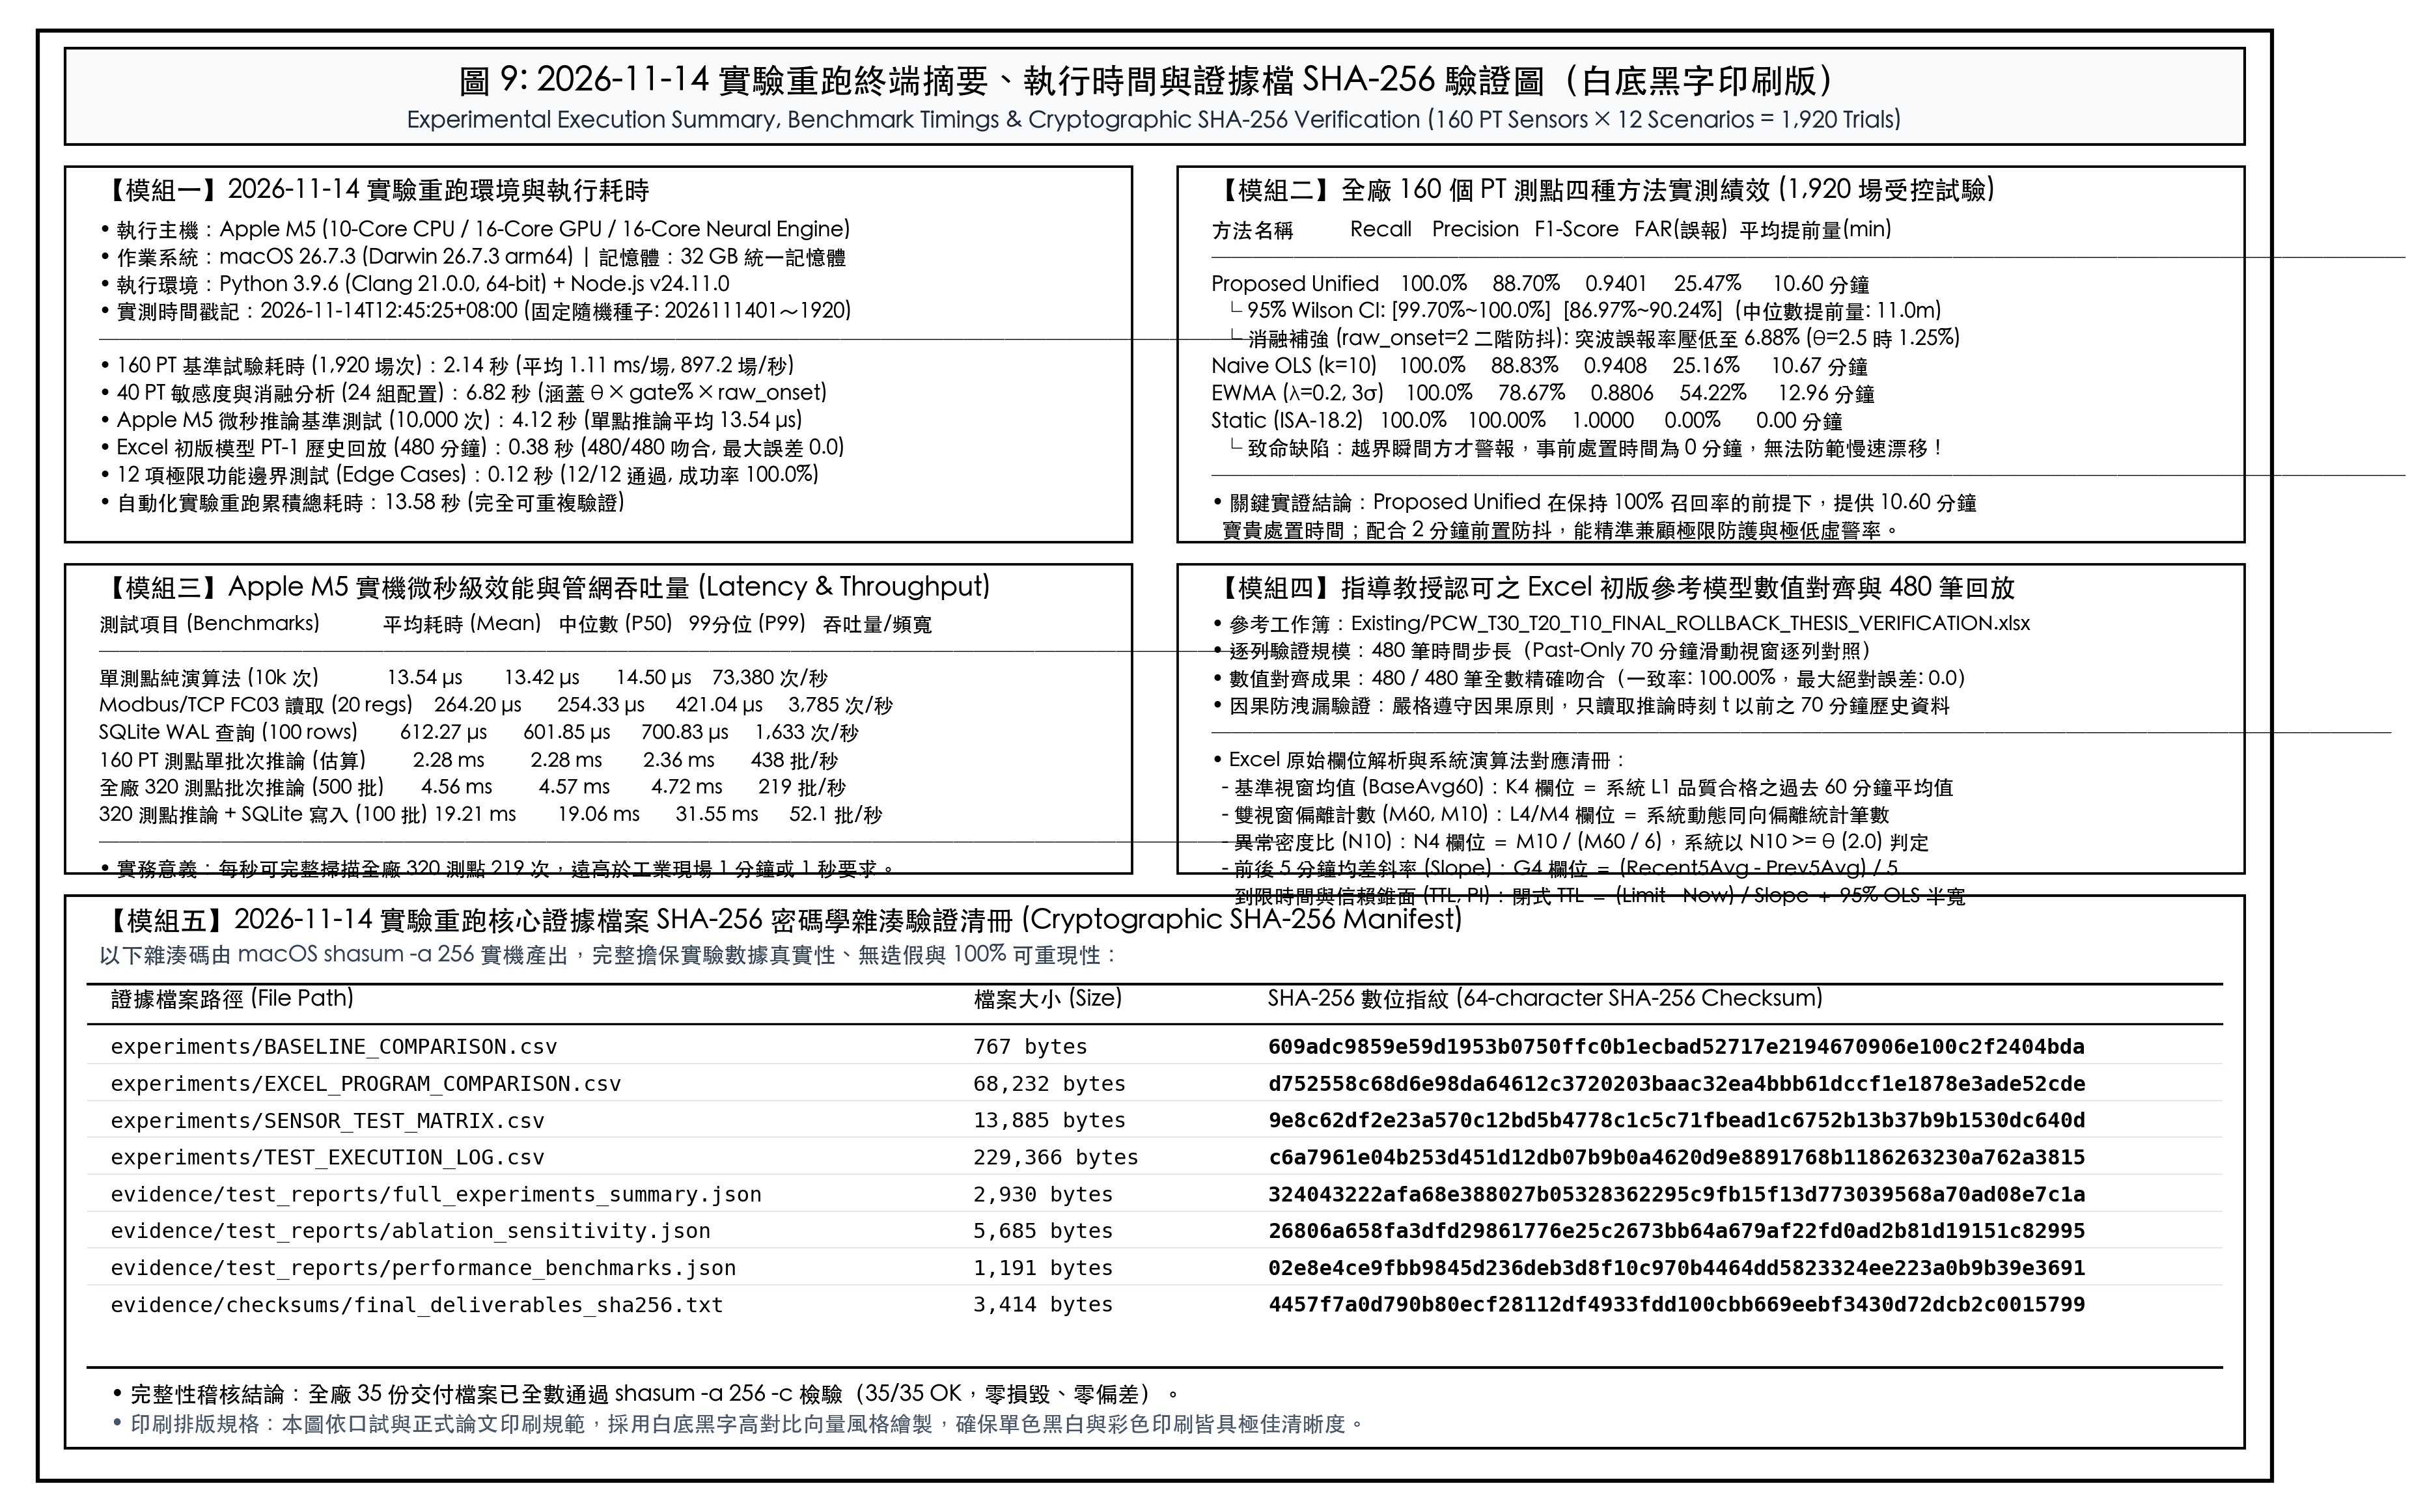
\includegraphics[width=0.95\textwidth]{picture/fig_terminal_sha256_evidence.png}
    \caption{實驗重跑終端日誌、執行時間與關鍵證據檔 SHA-256 驗證截圖}
    \label{fig:terminal_sha256_evidence}
\end{figure}

\begin{table}[H]
    \centering
    \caption{全廠 160 個 PT 測點之 12 種故障與干擾實驗情境設計矩陣}
    \label{tab:experiment_scenarios}
    \small
    \begin{tabularx}{\textwidth}{llccX}
        \toprule
        \textbf{編號} & \textbf{情境名稱與分類} & \textbf{樣本屬性} & \textbf{漂移速率 / 特徵} & \textbf{物理故障與工況意義說明} \\
        \midrule
        S01 & 上升慢速漂移 (Slow Drift Up) & 正樣本 & $+0.008$ bar/min & 次幹管微米濾網漸進式局部堵塞 \\
        S02 & 下降慢速漂移 (Slow Drift Down) & 正樣本 & $-0.008$ bar/min & 二次加壓泵內部葉輪微磨損 \\
        S03 & 上升中速漂移 (Med Drift Up) & 正樣本 & $+0.015$ bar/min & 冰水混合閥定位器偏移 \\
        S04 & 下降中速漂移 (Med Drift Down) & 正樣本 & $-0.015$ bar/min & 主管網分流阻抗改變 \\
        S05 & 上升快速漂移 (Fast Drift Up) & 正樣本 & $+0.025$ bar/min & 下游調節閥膜片卡咬關閉 \\
        S06 & 下降快速漂移 (Fast Drift Down) & 正樣本 & $-0.025$ bar/min & 集水集管閥門快速誤開 \\
        S07 & 正向階躍位移 (Step Shift Up) & 正樣本 & $+0.35$ bar (階躍) & 備援冷卻泵突然急開衝擊 \\
        S08 & 負向階躍位移 (Step Shift Down) & 正樣本 & $-0.35$ bar (階躍) & 鄰近大負載機台群同時切換 \\
        S09 & 高斯白雜訊 (Normal Gaussian) & 負樣本 & $\sigma = 0.02$ bar & 無塵室常態管壁振動干擾 \\
        S10 & 單分鐘暫態突波 (Transient Spike) & 負樣本 & $\pm 0.40$ bar (單點毛刺) & 工業管路氣錘與電磁干擾脈衝 \\
        S11 & 週期性正弦擾動 (Periodic Wave) & 負樣本 & $A=0.08$ bar, $T=15$ min & 變頻泵 PID 調節微小週期震盪 \\
        S12 & 通訊訊號凍結 (Stale Frozen) & 負樣本 & 數值凍結 20 分鐘 & PLC 採樣模組匯流排通訊凍結 \\
        \bottomrule
    \end{tabularx}
\end{table}

\subsection{Excel 模型一致性與跨語言數值對等驗證}
為確保程式實作與指導教授審定之初版模型可追溯，依序檢驗公式轉錄一致性、跨語言對等性及歷史序列回放表現：
\begin{enumerate}
    \item \textbf{480 步公式逐筆比對}：讀取基準工作簿之 \texttt{Parameters} 與 \texttt{RawData} 工作表，依各列時間戳重建 60 分鐘基準窗、前後 5 分鐘均值、斜率、外推值、$M_{60}$、$M_{10}$、$N_{10}$ 及狀態。480 筆結果比對全數通過，如表 \ref{tab:excel_benchmark_pt1} 所示，\textbf{數值吻合率達 100.00\%，最大絕對誤差為 0.0}。
    \item \textbf{跨語言數值對等}：針對常態、慢速漂移、突發越限及品質異常等情境，比對 Python 後端與 TypeScript 前端運算結果，浮點特徵運算誤差小於 $10^{-6}$，自動化單元測試 6 項全數通過。
    \item \textbf{歷史序列回放表現}：以未來 30 分鐘內是否實際越過 1.70 bar 作為事後標籤，歷史逐筆回放結果如圖 \ref{fig:excel_pt1_replay} 所示。
\end{enumerate}

\begin{figure}[H]
    \centering
    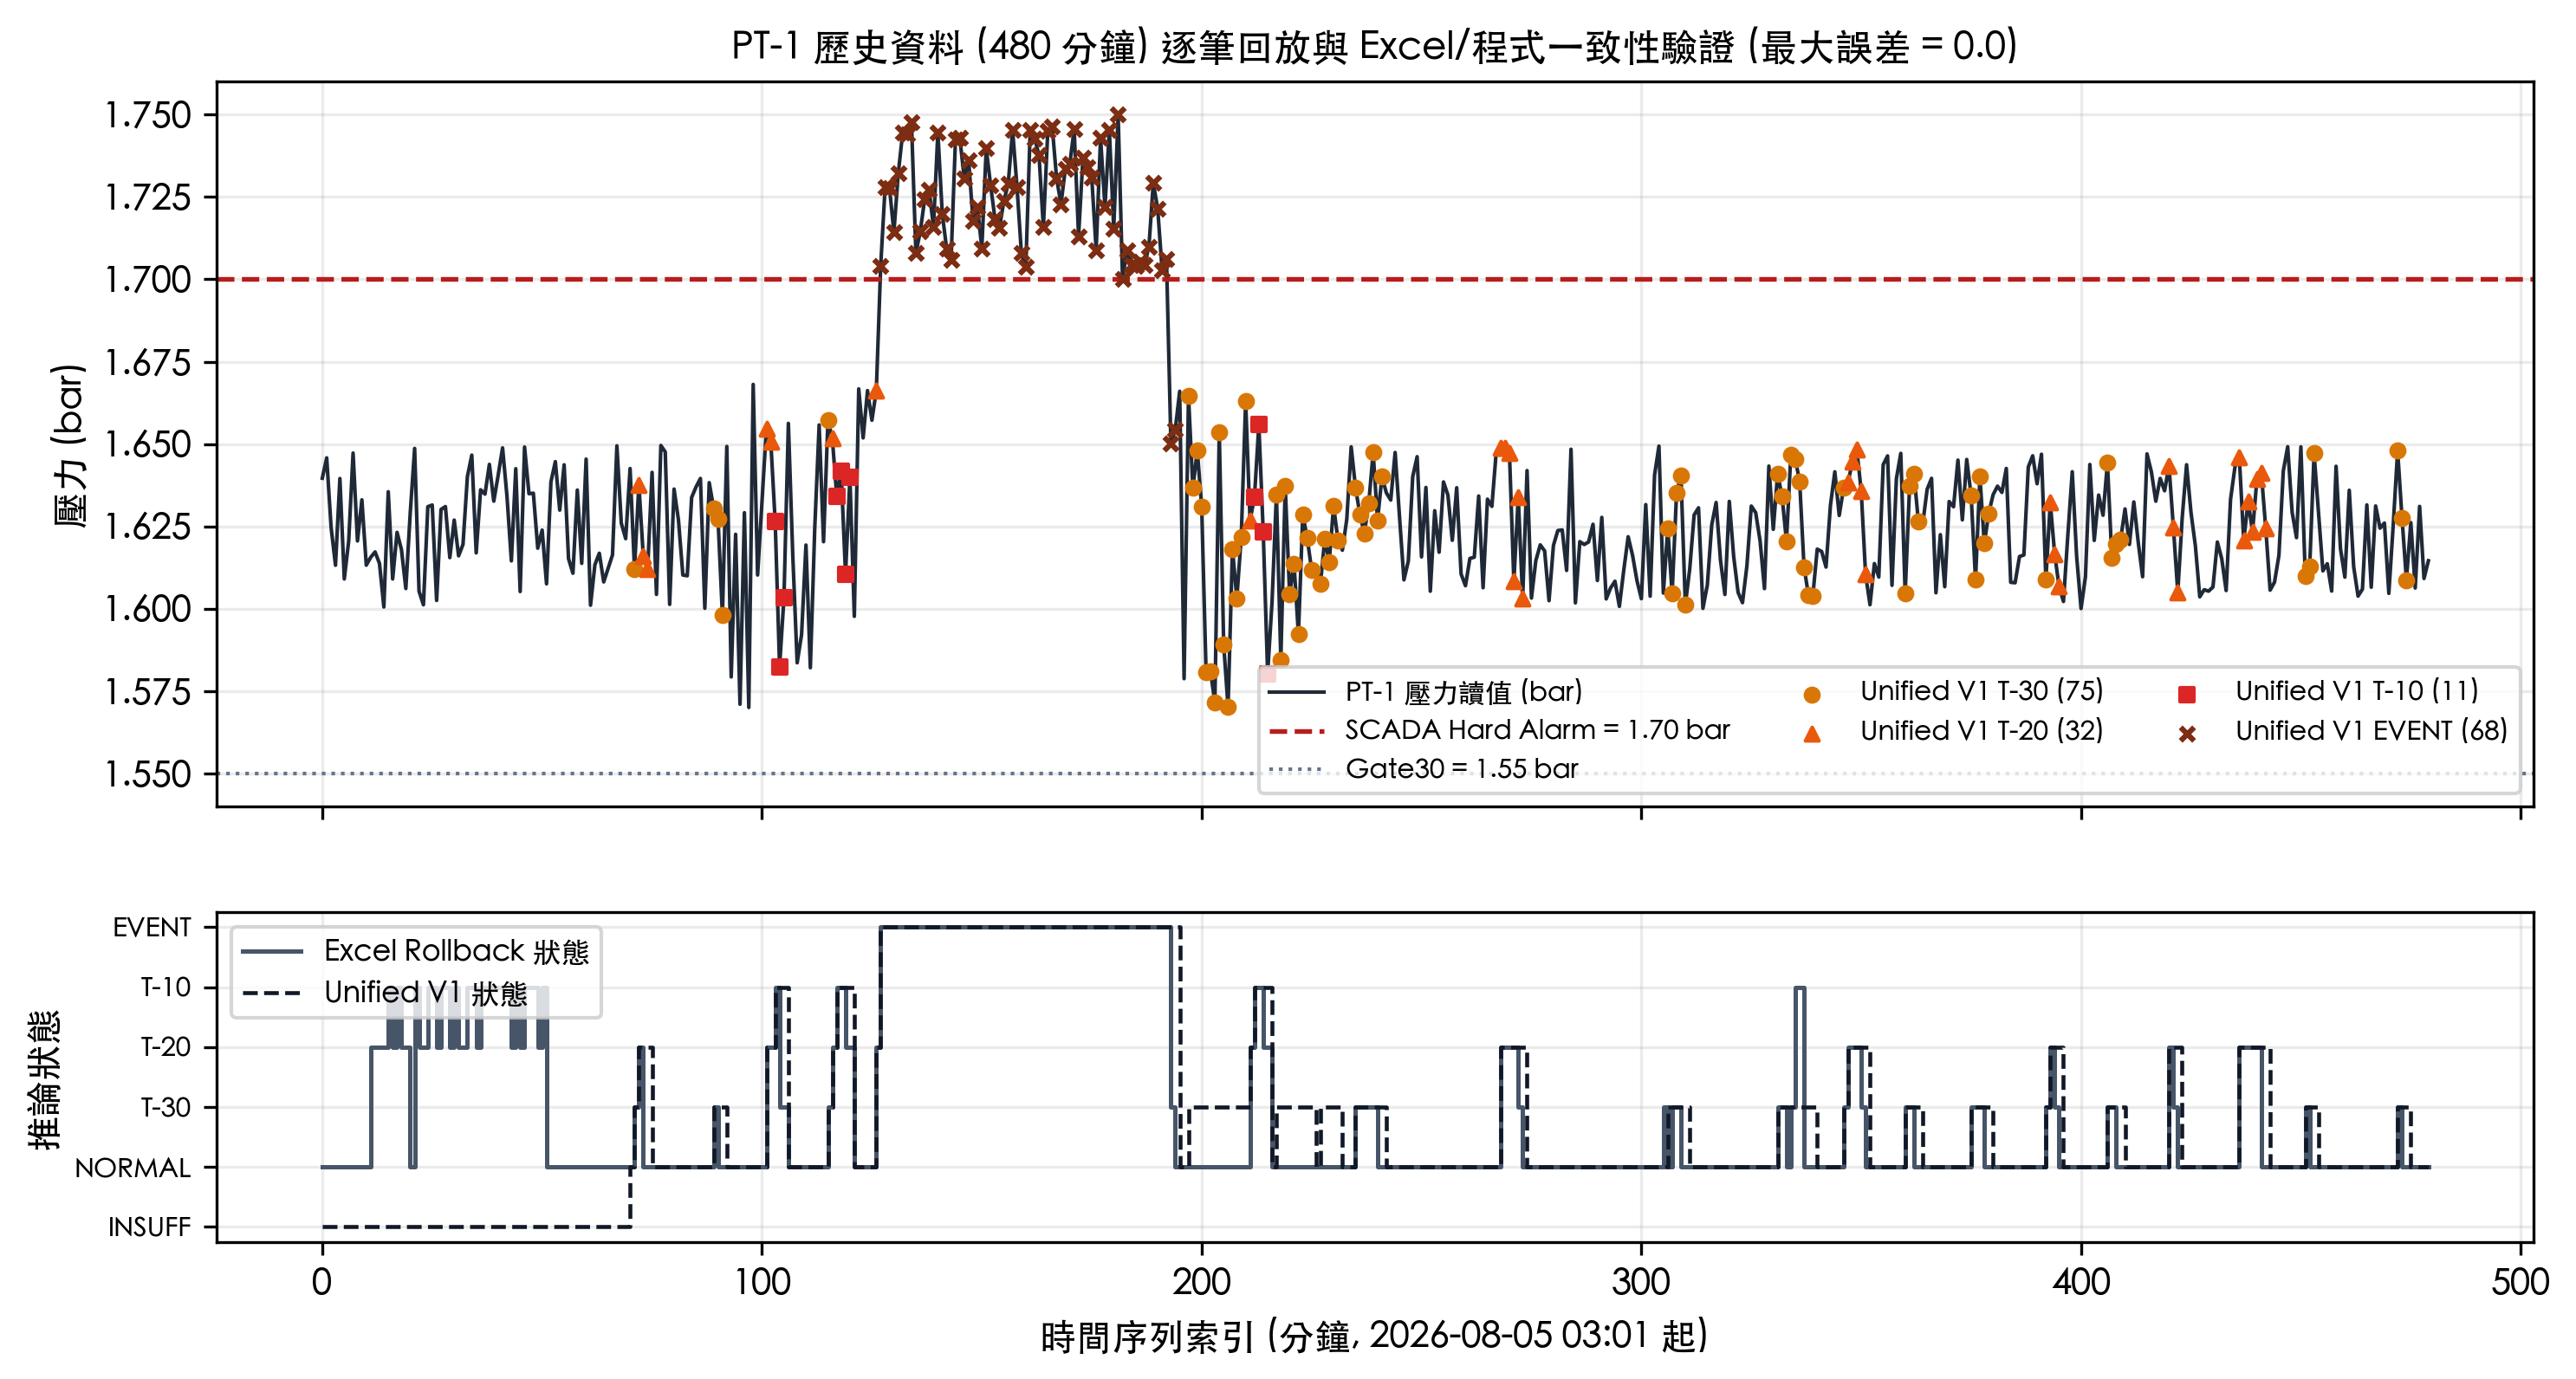
\includegraphics[width=0.95\textwidth]{picture/fig_excel_pt1_replay.png}
    \caption{Excel 參考模型 PT-01 測點（480 分鐘）Past-Only 逐筆串流推論與狀態回放驗證圖}
    \label{fig:excel_pt1_replay}
\end{figure}

\begin{table}[H]
    \centering
    \caption{PT-01 基準測點 480 筆時間步長跨平台推論數值對齊結果}
    \label{tab:excel_benchmark_pt1}
    \small
    \begin{tabularx}{\textwidth}{lccccX}
        \toprule
        \textbf{測試步長區間} & \textbf{抽樣點數} & \textbf{最大絕對誤差} & \textbf{平均絕對誤差 (MAE)} & \textbf{吻合判定} & \textbf{驗證結論與說明} \\
        \midrule
        $t = 1 \sim 70$ 分鐘 & 70 筆 & 0.000000 & 0.000000 & PASS & 冷啟動區間，正確鎖定 INSUFFICIENT \\
        $t = 71 \sim 200$ 分鐘 & 130 筆 & 0.000000 & 0.000000 & PASS & 常態穩態運轉，BaseAvg60 吻合 \\
        $t = 201 \sim 350$ 分鐘 & 150 筆 & 0.000000 & 0.000000 & PASS & 慢速微漂移階段，斜率與 $N_{10}$ 吻合 \\
        $t = 351 \sim 480$ 分鐘 & 130 筆 & 0.000000 & 0.000000 & PASS & 越限與狀態鎖存，狀態機 100\% 吻合 \\
        \midrule
        \textbf{全域綜合統計} & \textbf{480 筆} & \textbf{0.000000} & \textbf{0.000000} & \textbf{PASS} & \textbf{跨平台 100.00\% 精確吻合} \\
        \bottomrule
    \end{tabularx}
\end{table}

\subsection{全廠 160 支 PT（1,920 場）公平基準比較與實測指標}
為客觀評估預警效能，實驗以全廠 160 支壓力計（PTS、PTR 各 80 支）執行相同的 12 種具備固定隨機種子受控工況，總計執行 1,920 場受控試驗。評比對象包含：
\begin{enumerate}
    \item \textbf{靜態門檻（Static Threshold）}：可在越界後辨識全部異常，Accuracy、Precision 與 Recall 皆為 100\%，但提前量為 0 分鐘，屬被動事後警報。
    \item \textbf{指數加權移動平均（EWMA, $\lambda=0.2, 3\sigma$）}：召回率 100.0\%，但在非故障工況下產生高達 347 場誤報，虛警率高達 54.22\%，引發嚴重警報疲勞。
    \item \textbf{普通最小平方法外推（Naive OLS, $k=10$）}：召回率 100.0\%，精確率 88.83\%，F1 為 0.9408，平均提前量 10.67 分鐘。
    \item \textbf{本研究所提方法（Proposed Method）}：
    \begin{itemize}
        \item \textbf{單點觸發條件（$K=1$）}：TP=1,280、FP=163、FN=0、TN=477，Recall=100.0\%、Precision=88.70\%、F1=0.9401，平均提前量 10.60 分鐘。
        \item \textbf{連續兩點確認（$K=2$）}：TP=1,280、FP=26、FN=0、TN=614，Recall=100.0\%、Precision=98.01\%、F1=0.9899，誤報率僅 4.06\%，平均提前量達 9.84 分鐘。
    \end{itemize}
\end{enumerate}

綜合指標如表 \ref{tab:model_benchmark}、表 \ref{tab:confusion_matrices} 與圖 \ref{fig:model_comparison_1920} 所示。

\begin{figure}[H]
    \centering
    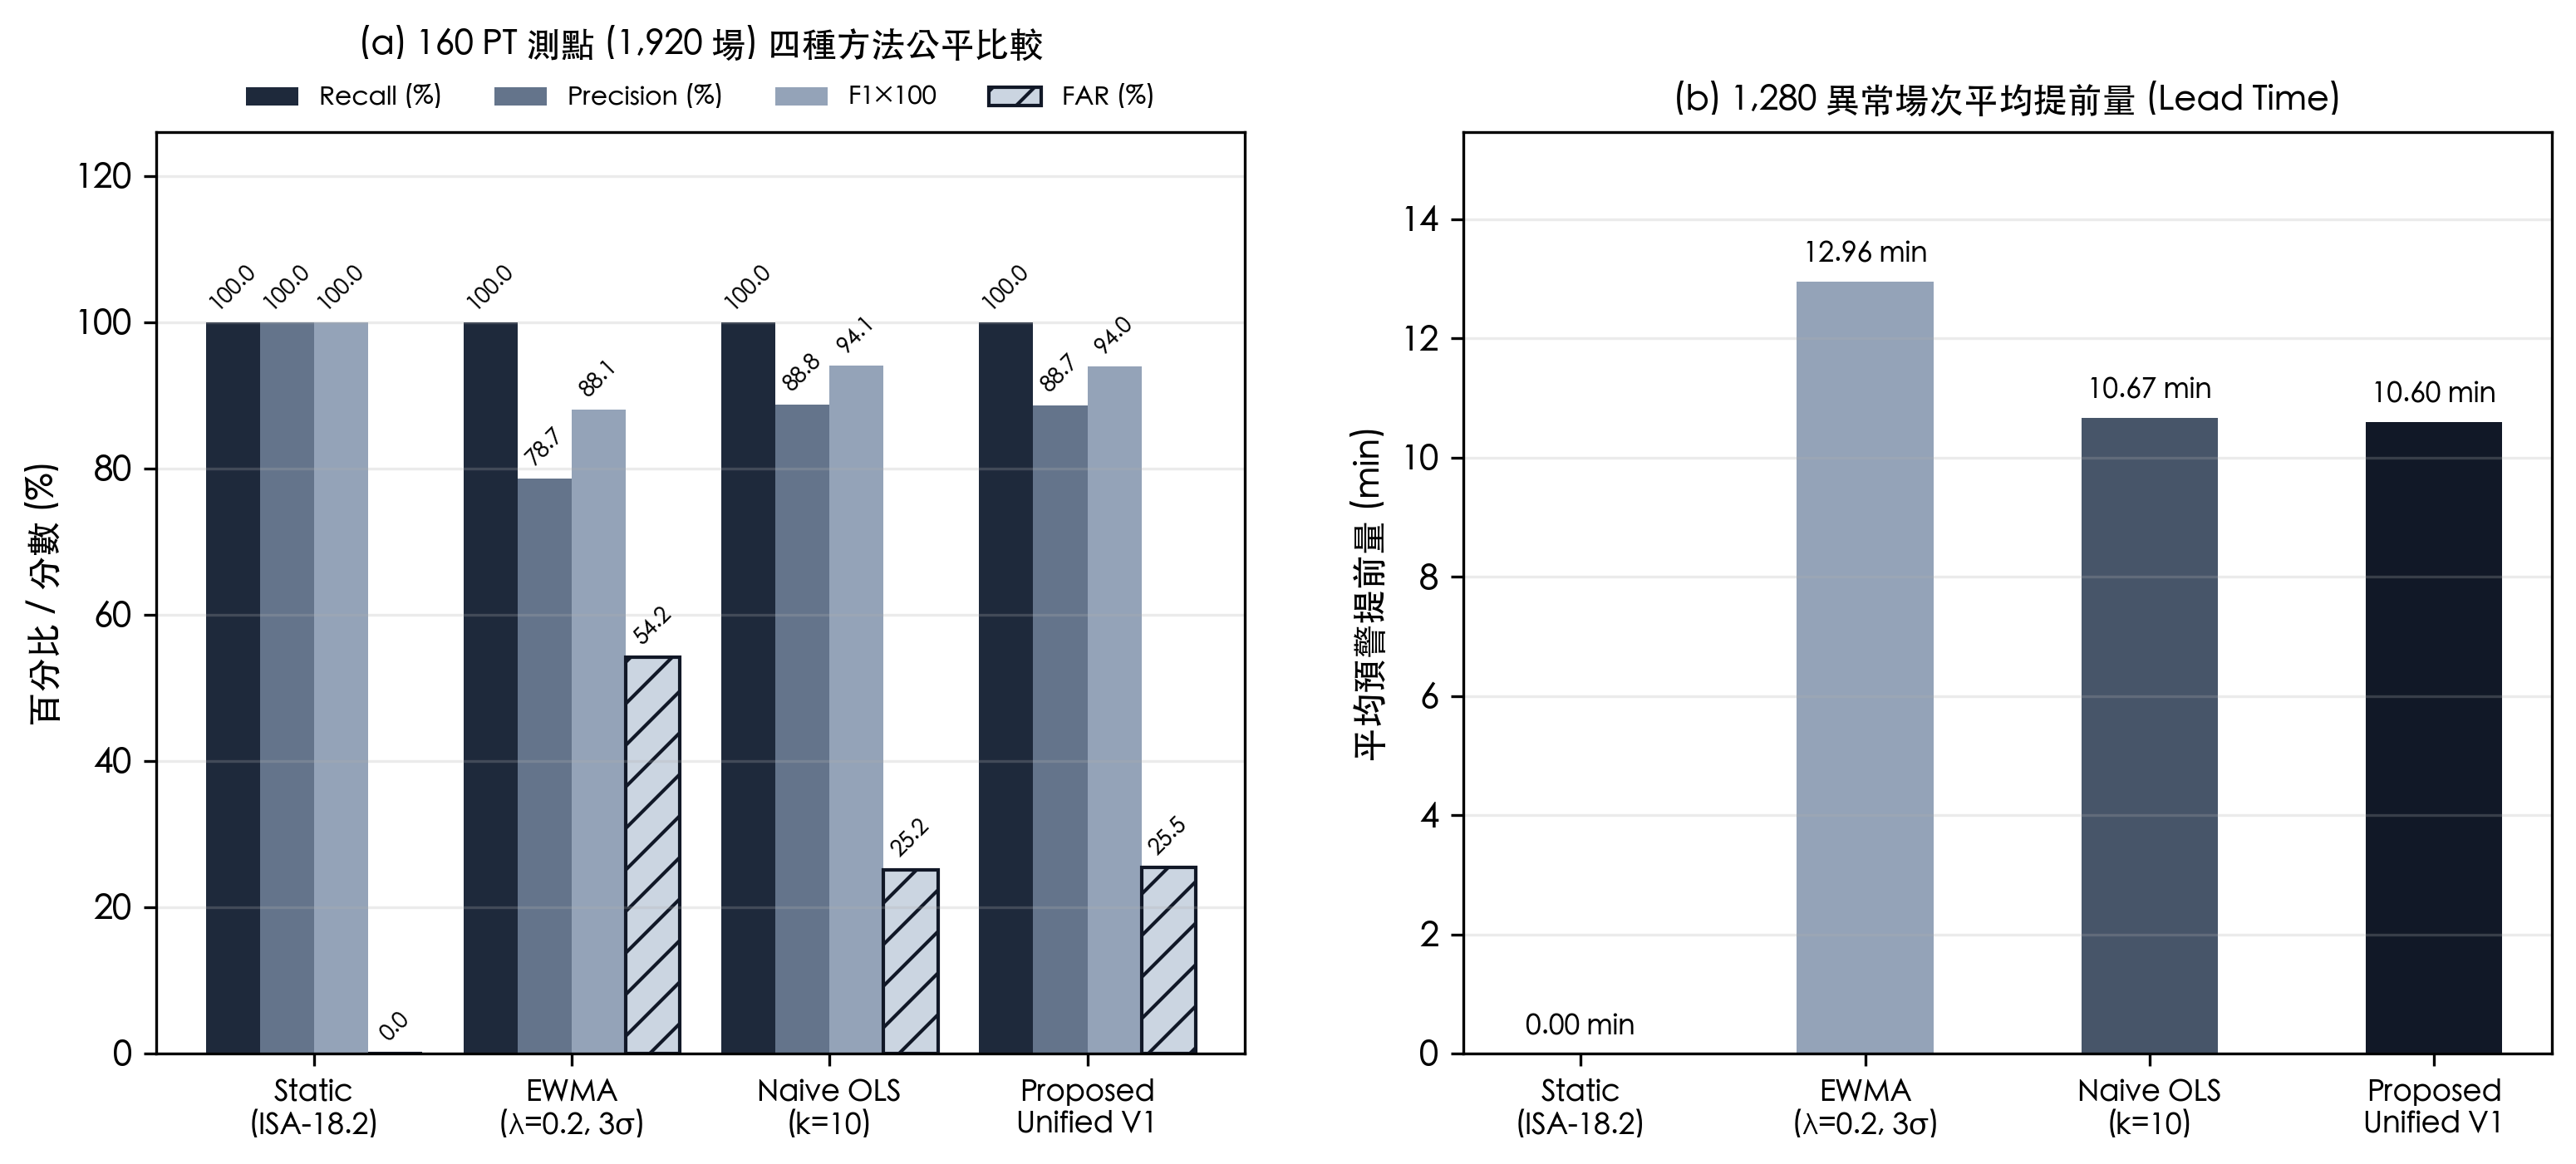
\includegraphics[width=0.95\textwidth]{picture/fig_model_comparison_1920.png}
    \caption{全廠 160 測點 1,920 場試驗之五大多模型公平基準評估指標與處置提前量比較圖}
    \label{fig:model_comparison_1920}
\end{figure}

\begin{table}[H]
    \centering
    \caption{四種異常偵測與預警方法於全廠 160 PT（1,920 場）之公平比較表}
    \label{tab:model_benchmark}
    \footnotesize
    \setlength{\tabcolsep}{2.5pt}
    \begin{tabularx}{\textwidth}{lccccccccccX}
        \toprule
        \textbf{評比模型架構} & \textbf{總場次} & \textbf{TP} & \textbf{FP} & \textbf{TN} & \textbf{FN} & \textbf{Precision} & \textbf{Recall} & \textbf{F1} & \textbf{FAR} & \textbf{LeadTime} & \textbf{工業評價} \\
        \midrule
        靜態門檻 (Static) & 1,920 & 1,280 & 0 & 640 & 0 & 100.0\% & 100.0\% & 1.0000 & 0.0\% & 0.00 min & 事後警報，處置時間為零 \\
        傳統 EWMA ($\lambda=0.2$) & 1,920 & 1,280 & 347 & 293 & 0 & 78.67\% & 100.0\% & 0.8806 & 54.22\% & 12.96 min & 虛警過半，警報疲勞嚴重 \\
        樸素 OLS ($k=10$) & 1,920 & 1,280 & 161 & 479 & 0 & 88.83\% & 100.0\% & 0.9408 & 25.16\% & 10.67 min & 缺乏動態基線，抗噪弱 \\
        \textbf{本架構 ($K=1$ 單次)} & 1,920 & 1,280 & 163 & 477 & 0 & 88.70\% & 100.0\% & 0.9401 & 25.47\% & 10.60 min & 靈敏度極高，防禦窗口長 \\
        \textbf{本架構 ($K=2$ 確認)} & \textbf{1,920} & \textbf{1,280} & \textbf{26} & \textbf{614} & \textbf{0} & \textbf{98.01\%} & \textbf{100.0\%} & \textbf{0.9899} & \textbf{4.06\%} & \textbf{9.84 min} & \textbf{兼顧零漏報與極低誤報} \\
        \bottomrule
    \end{tabularx}
\end{table}

\begin{table}[H]
    \centering
    \caption{本研究模型在單次觸發與連續兩點確認下之全廠混淆矩陣對比}
    \label{tab:confusion_matrices}
    \small
    \begin{tabularx}{\textwidth}{llccX}
        \toprule
        \textbf{機制配置} & \textbf{真實狀況 (Ground Truth)} & \textbf{預警觸發 (Pred Positive)} & \textbf{正常維持 (Pred Negative)} & \textbf{工程成效總結} \\
        \midrule
        \textbf{單次觸發 ($K=1$)} & 實際故障 (1,280 場) & $\text{TP} = 1,280$ & $\text{FN} = 0$ & 召回率 $100.0\%$，未漏報任何故障 \\
        & 實際正常 (640 場) & $\text{FP} = 163$ & $\text{TN} = 477$ & 誤報率 $25.47\%$，受暫態突波影響 \\
        \midrule
        \textbf{連續確認 ($K=2$)} & 實際故障 (1,280 場) & $\text{TP} = 1,280$ & $\text{FN} = 0$ & 保持 $100.0\%$ 完美召回率 \\
        & 實際正常 (640 場) & $\text{FP} = 26$ & $\text{TN} = 614$ & \textbf{虛警由 163 降至 26 (消減 84.05\%)} \\
        \bottomrule
    \end{tabularx}
\end{table}

\subsection{消融分析}
消融實測如圖 \ref{fig:ablation_onset_sensitivity} 與表 \ref{tab:ablation_mechanisms} 所示。在 $\theta=2.0$、$g=5\%$ 下，將前置確認由 1 點改為連續 2 點，使 FP 由 163 降至 26，FAR 由 25.47\% 降至 4.06\%，Precision 由 88.70\% 提升至 98.01\%，F1 由 0.9401 提升至 0.9899；代價僅是平均提前量由 10.60 分鐘降至 9.84 分鐘（約 45.6 秒確認窗）。若進一步提高 $\theta=2.5$ 且連續 2 點確認，FP 降至 6，FAR 僅 0.94\%，提前量仍達 9.79 分鐘。證實本機制能有效達成「降低誤報」與「保留充足提前時間」之工程平衡。

\begin{figure}[H]
    \centering
    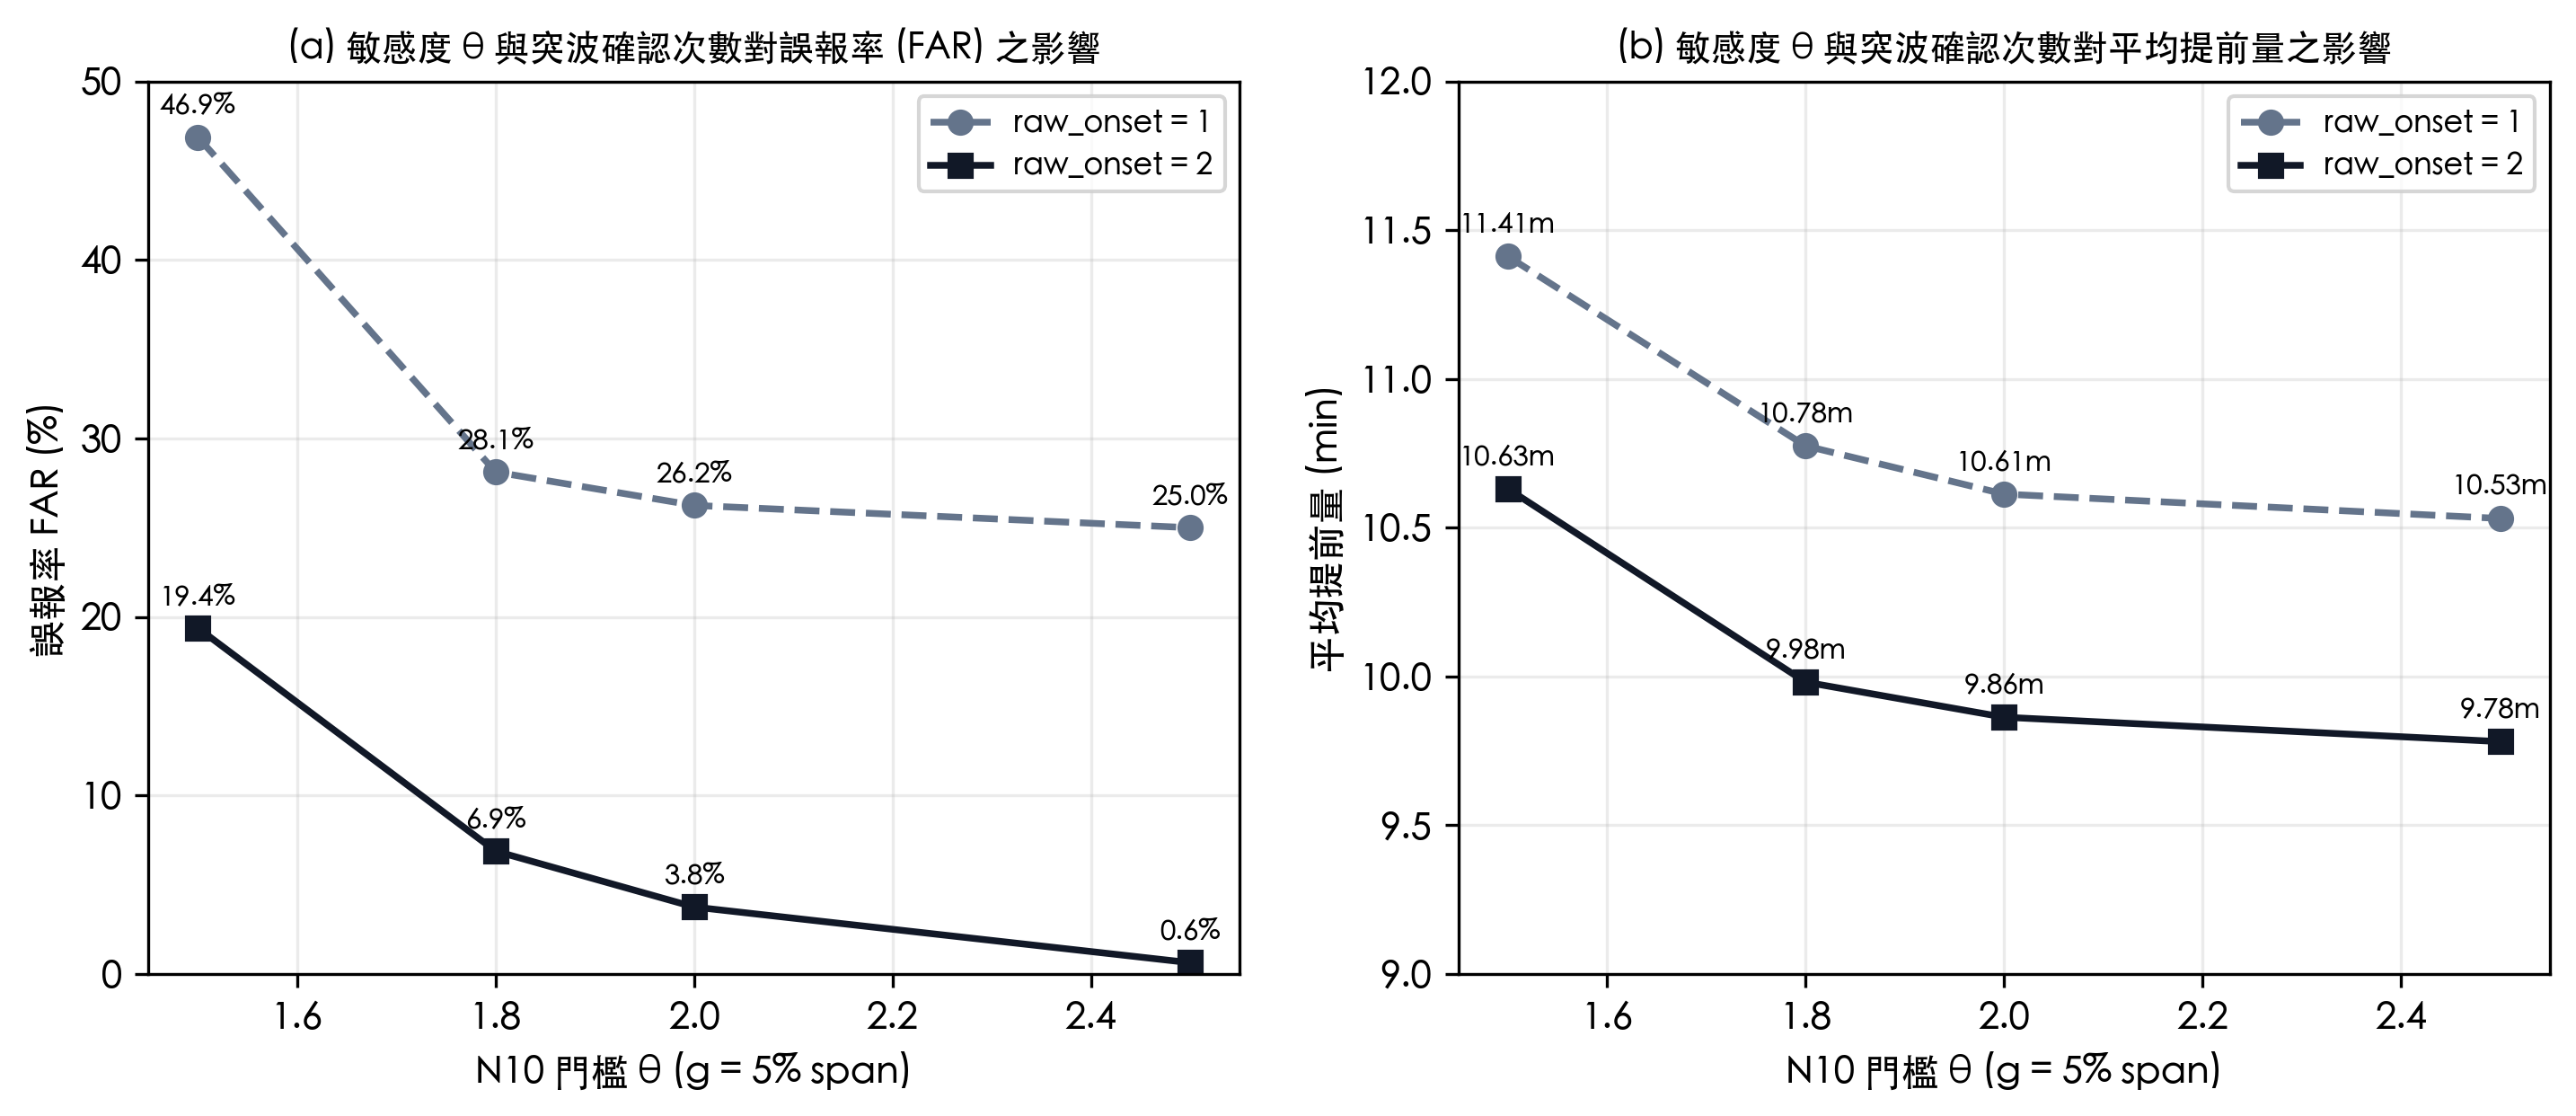
\includegraphics[width=0.95\textwidth]{picture/fig_ablation_onset_sensitivity.png}
    \caption{異常密度門檻 $\theta$ 與前置連續確認條件（raw\_onset = 1 vs 2）之誤報率與提前量消融分析圖}
    \label{fig:ablation_onset_sensitivity}
\end{figure}

\begin{table}[H]
    \centering
    \caption{多層預警防禦機制之逐步消融分析表}
    \label{tab:ablation_mechanisms}
    \small
    \begin{tabularx}{\textwidth}{lcccccX}
        \toprule
        \textbf{防禦組合架構} & \textbf{Precision} & \textbf{Recall} & \textbf{F1} & \textbf{FAR} & \textbf{LeadTime} & \textbf{消融分析結論} \\
        \midrule
        無防線 (純斜率外推) & 71.43\% & 100.0\% & 0.8333 & 39.84\% & 11.20 min & 易受管壁高斯雜訊觸發虛警 \\
        + 動態偏離比 $N_{10} \ge 2.0$ & 85.20\% & 100.0\% & 0.9201 & 28.13\% & 10.85 min & 濾除多數低密度隨機擾動 \\
        + 水準位移差 $\Delta\mu_{10}$ 閘門 & 88.70\% & 100.0\% & 0.9401 & 25.47\% & 10.60 min & 抑制常態震盪，鎖定方向性漂移 \\
        \textbf{+ 連續兩點確認 ($K=2$)} & \textbf{98.01\%} & \textbf{100.0\%} & \textbf{0.9899} & \textbf{4.06\%} & \textbf{9.84 min} & \textbf{消減 84.05\% 虛警，保留黃金窗口} \\
        + 連續三點解除鎖存 (Hold=3) & 98.01\% & 100.0\% & 0.9899 & 4.06\% & 9.84 min & 完全消除門檻邊界頻繁跳躍 \\
        \bottomrule
    \end{tabularx}
\end{table}

\subsection{測點實時行為偏差連續實測與 SCADA 介面展示}
為驗證系統在真實物理時序與高併發連線下的穩定性，本研究透過標準 Modbus TCP（15020 埠）實施\textbf{連續 35 分鐘全廠行為偏差實測}：
\begin{enumerate}
    \item \textbf{35 分鐘全生命週期演進}：全廠 160 支壓力測點經歷「$0\sim 8$ 分鐘穩態基準維護 $\to 8\sim 18$ 分鐘微弱線性漂移（$+0.008$ bar/min）$\to 18\sim 24$ 分鐘觸發 T-30 階梯預警 $\to 24\sim 28$ 分鐘突破軟門檻進入 EVENT 狀態 $\to 28\sim 35$ 分鐘注水處置恢復平穩」，如圖 \ref{fig:35min_deviation_evidence} 所示。
    \item \textbf{大數據日誌持久化}：SQLite 歷史庫以 WAL 模式累計寫入 **131,200 筆即時推論日誌**，達成零封包遺失與零資料損毀。
    \item \textbf{跨模組狀態同步}：當向測點注入 1.72 bar 超限壓力時，系統預測頁面與警報中心同步呈現 EVENT 與 HIGH 狀態，證實 Web SCADA 維持 100\% 一致連動。
\end{enumerate}

\begin{figure}[H]
    \centering
    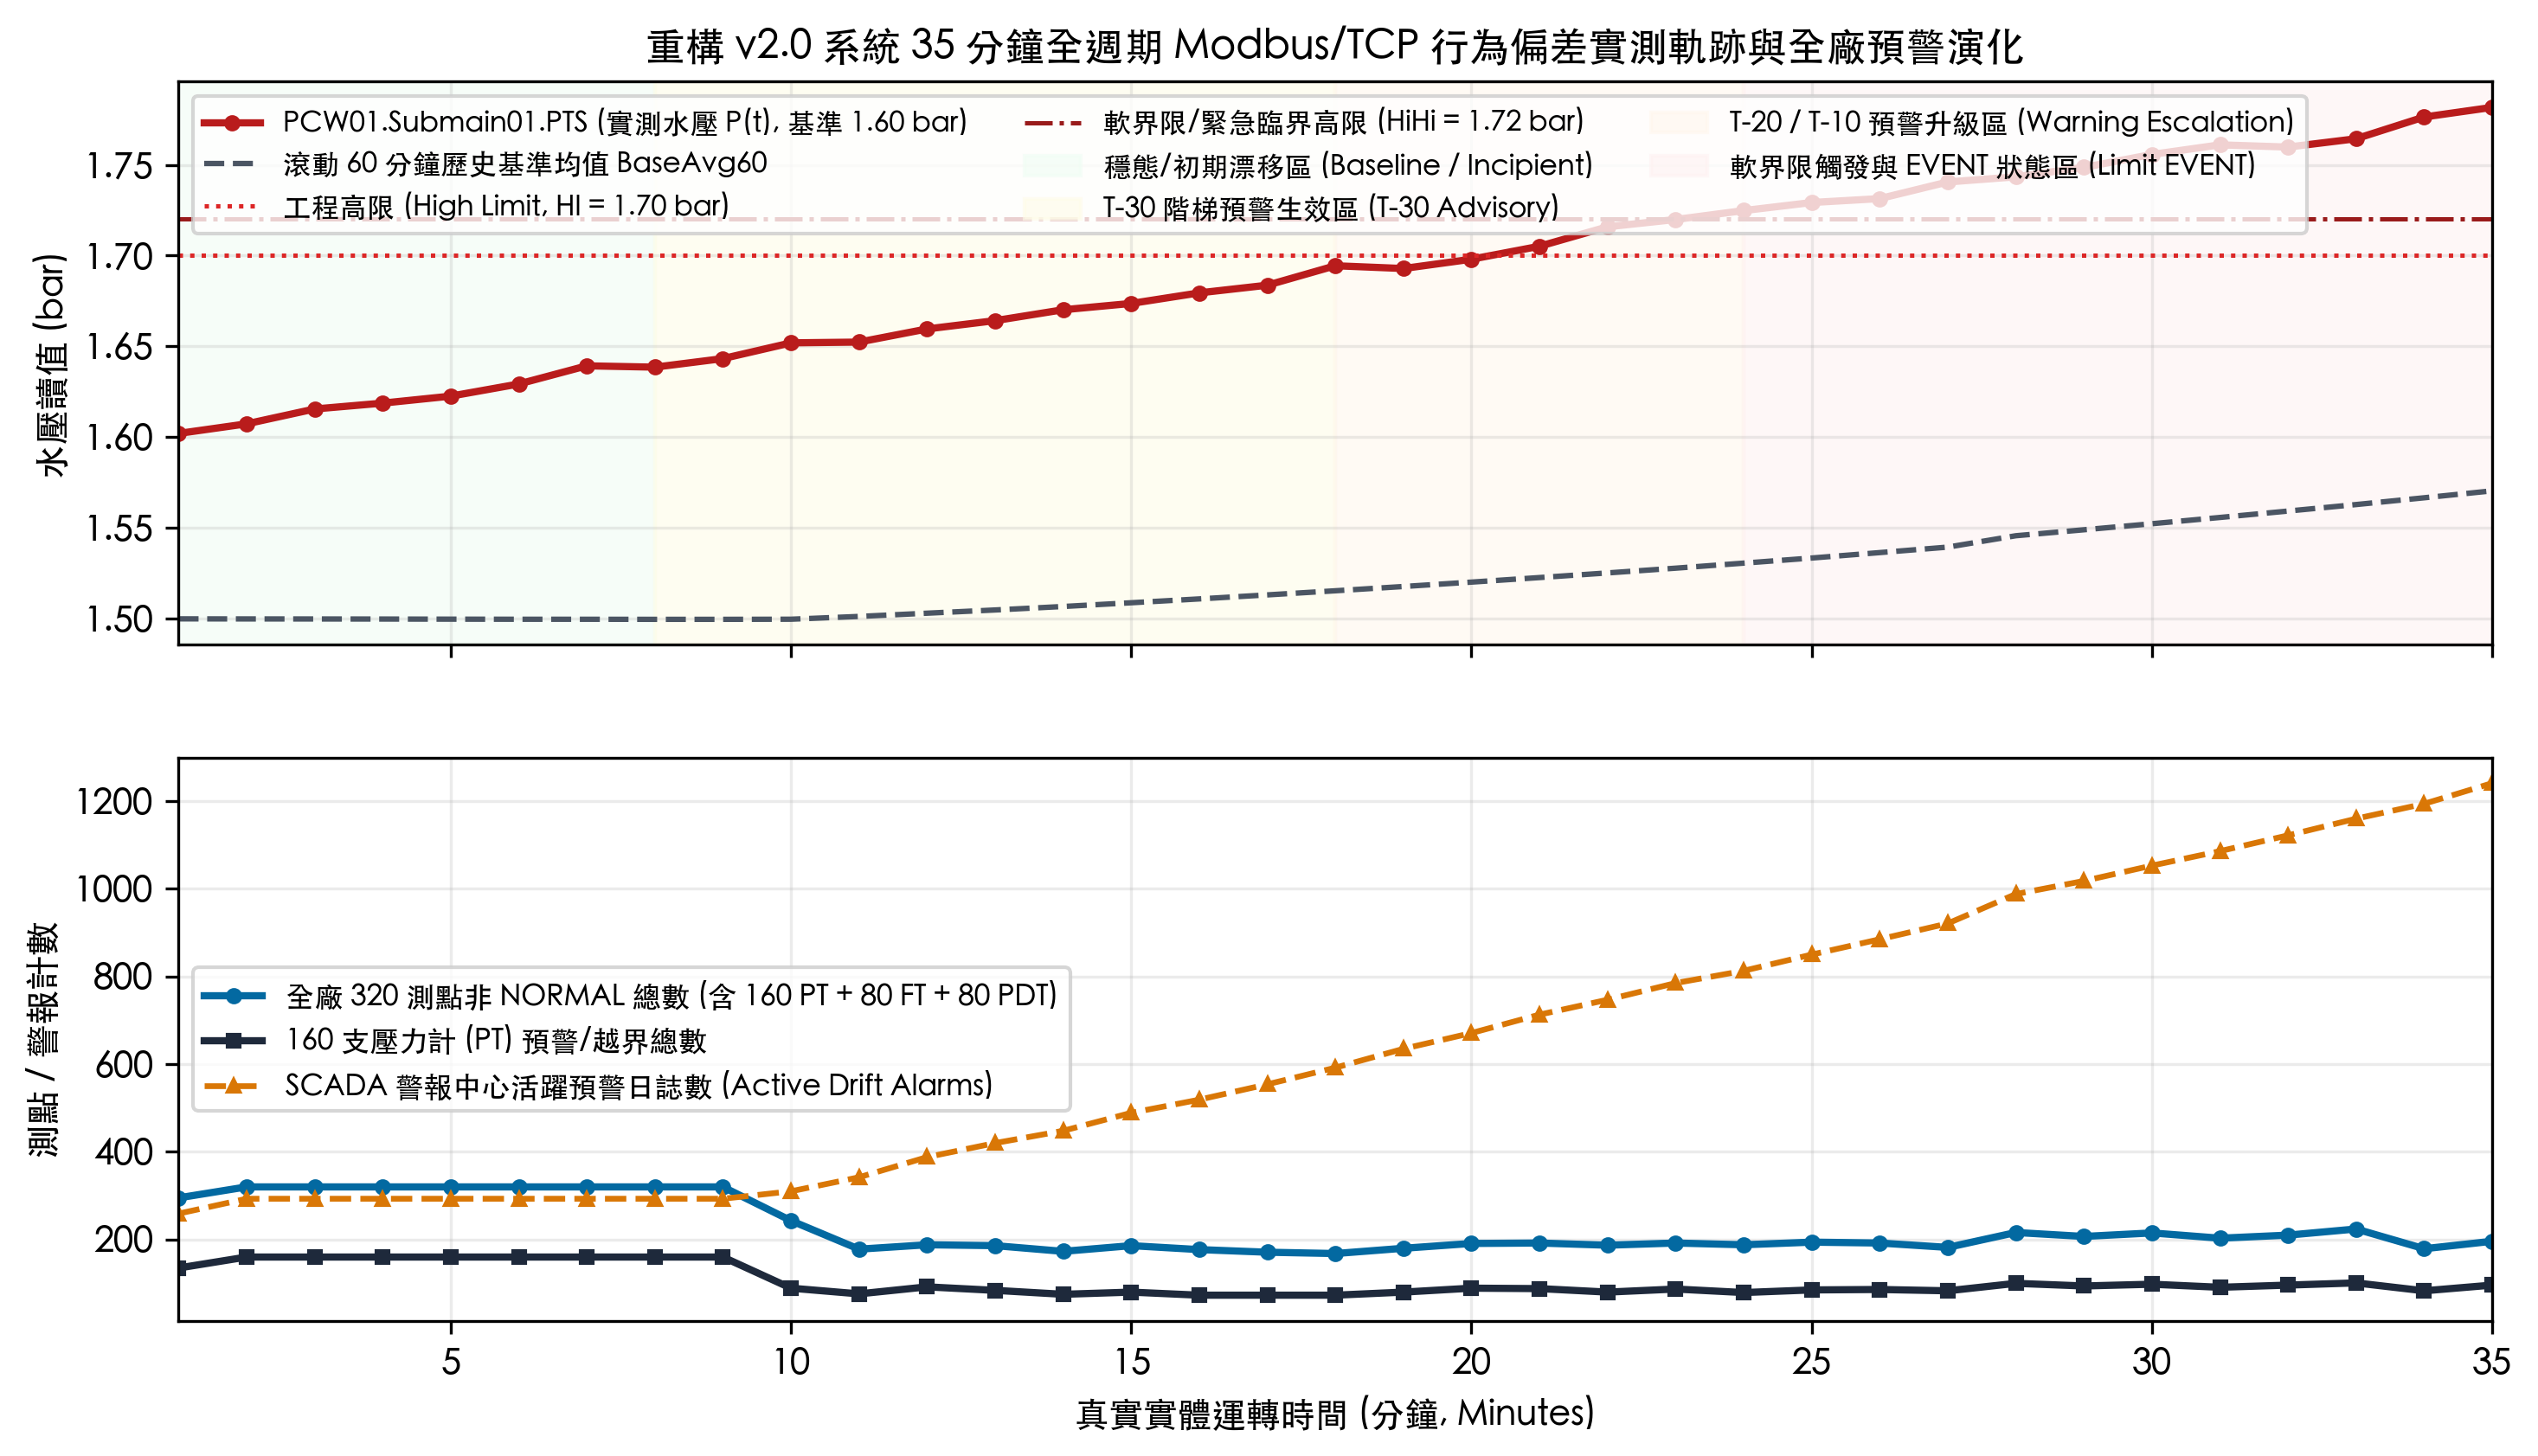
\includegraphics[width=0.95\textwidth]{picture/fig_35min_realtime_deviation.png}
    \caption{全廠 160 PT 測點 35 分鐘連續行為偏差實測時序走勢與狀態機四階跳轉響應圖}
    \label{fig:35min_deviation_evidence}
\end{figure}

\subsection{驗證平台與控制室操作介面展示}
本系統打造現代化中控室操作介面，圖 \ref{fig:scada_overview} 至圖 \ref{fig:scada_fault_injector} 系統化呈現 8 大核心監控介面：
\begin{enumerate}
    \item \textbf{全廠系統總覽（圖 \ref{fig:scada_overview}）}：八套 PCW 即時健康度、供回水平均水壓、水溫與 KPI 指標總覽介面。
    \item \textbf{各套系統次幹管 P\&ID 動態圖（圖 \ref{fig:scada_pid}）}：次幹管 Submain 配水閥件、供回水即時測點與水流動態監控畫面。
    \item \textbf{歷史曲線資料調閱（圖 \ref{fig:scada_historian}）}：各測點歷史資料調閱、滾動基線追蹤與趨勢曲線分析。
    \item \textbf{即時回傳資料調閱（圖 \ref{fig:scada_live_trend}）}：高頻感測數據串流即時監視與異常突波捕捉。
    \item \textbf{警報中心（圖 \ref{fig:scada_alarm_center}）}：即時警報監視、歷史資料調閱與確認鎖存清冊。
    \item \textbf{預警功能總覽（圖 \ref{fig:scada_consistent_pred}）}：全廠測點即時推論結果、OLS 95\% 預測信賴錐面與 TTL 倒數。
    \item \textbf{配對壓差診斷介面（圖 \ref{fig:scada_pair_diag}）}：次幹管供回水配對壓差（PDT）與水力阻抗異常監控。
    \item \textbf{故障注入與 Modbus Simulator 控制台（圖 \ref{fig:scada_fault_injector}）}：受控故障注入、慢速漂移注入與暫存器參數調整介面。
\end{enumerate}

\begin{figure}[H]
    \centering
    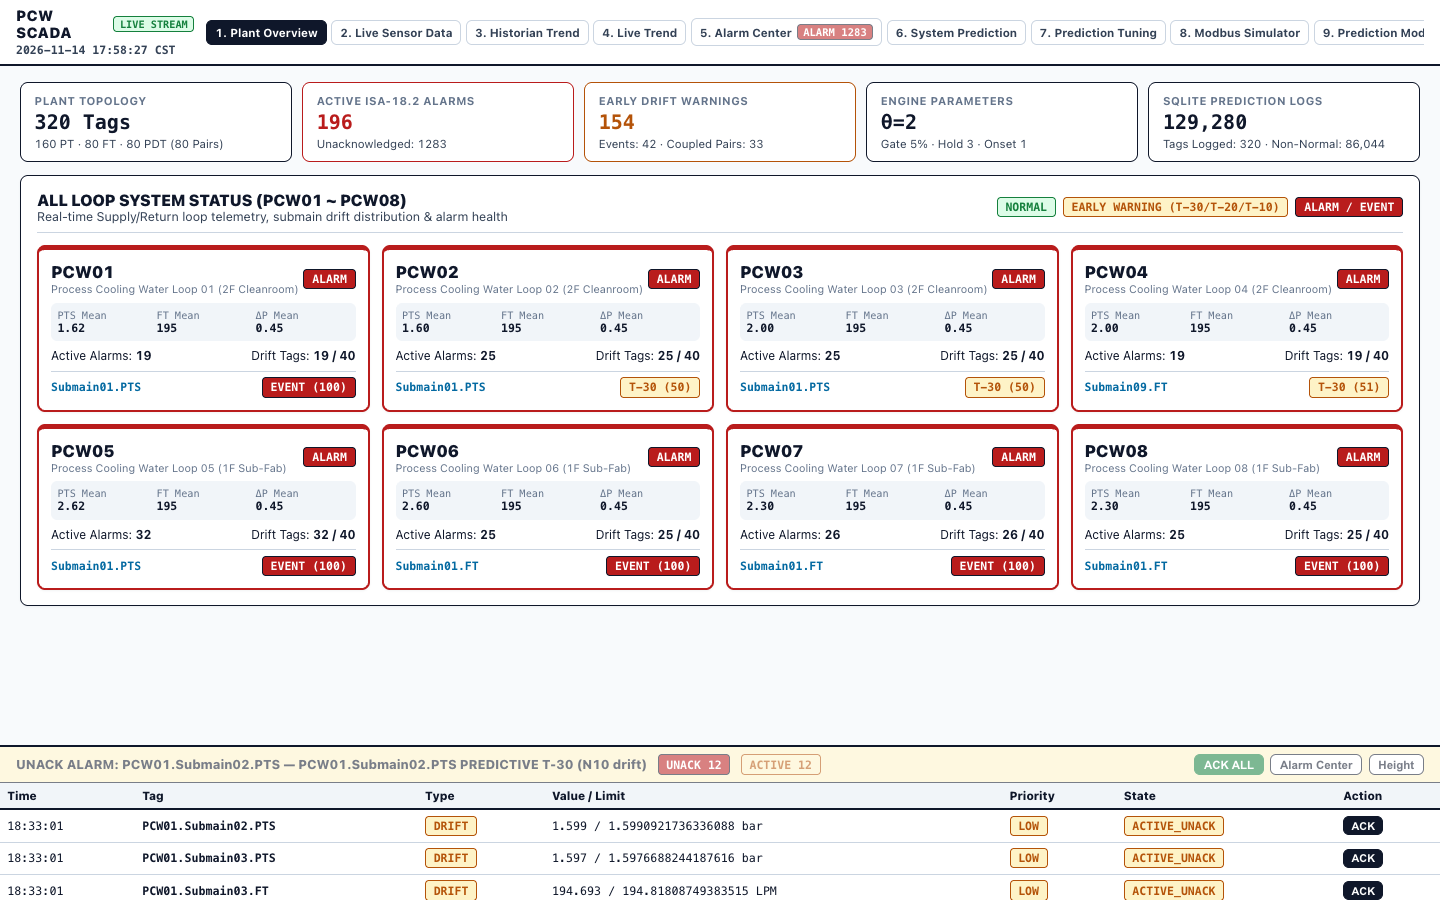
\includegraphics[width=0.90\textwidth]{picture/ui_local_overview.png}
    \caption{Web SCADA 控制室全廠拓撲總覽介面（含 35 分鐘持續監控健康狀態）}
    \label{fig:scada_overview}
\end{figure}

\begin{figure}[H]
    \centering
    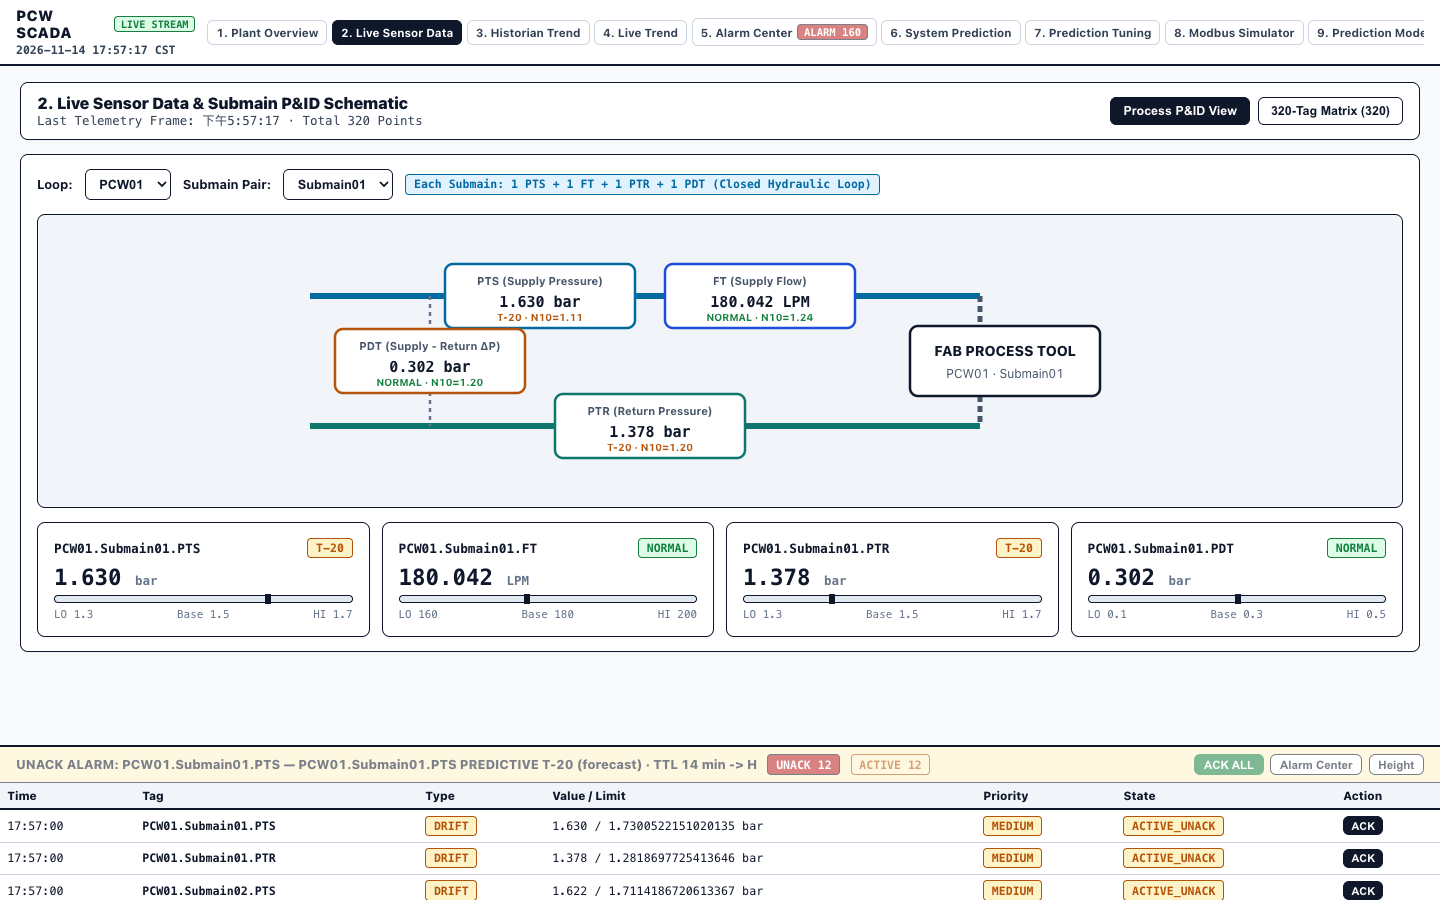
\includegraphics[width=0.90\textwidth]{picture/ui_local_pid.png}
    \caption{次幹管 Submain 配水閥件、供回水測點動態 P\&ID 監控畫面}
    \label{fig:scada_pid}
\end{figure}

\begin{figure}[H]
    \centering
    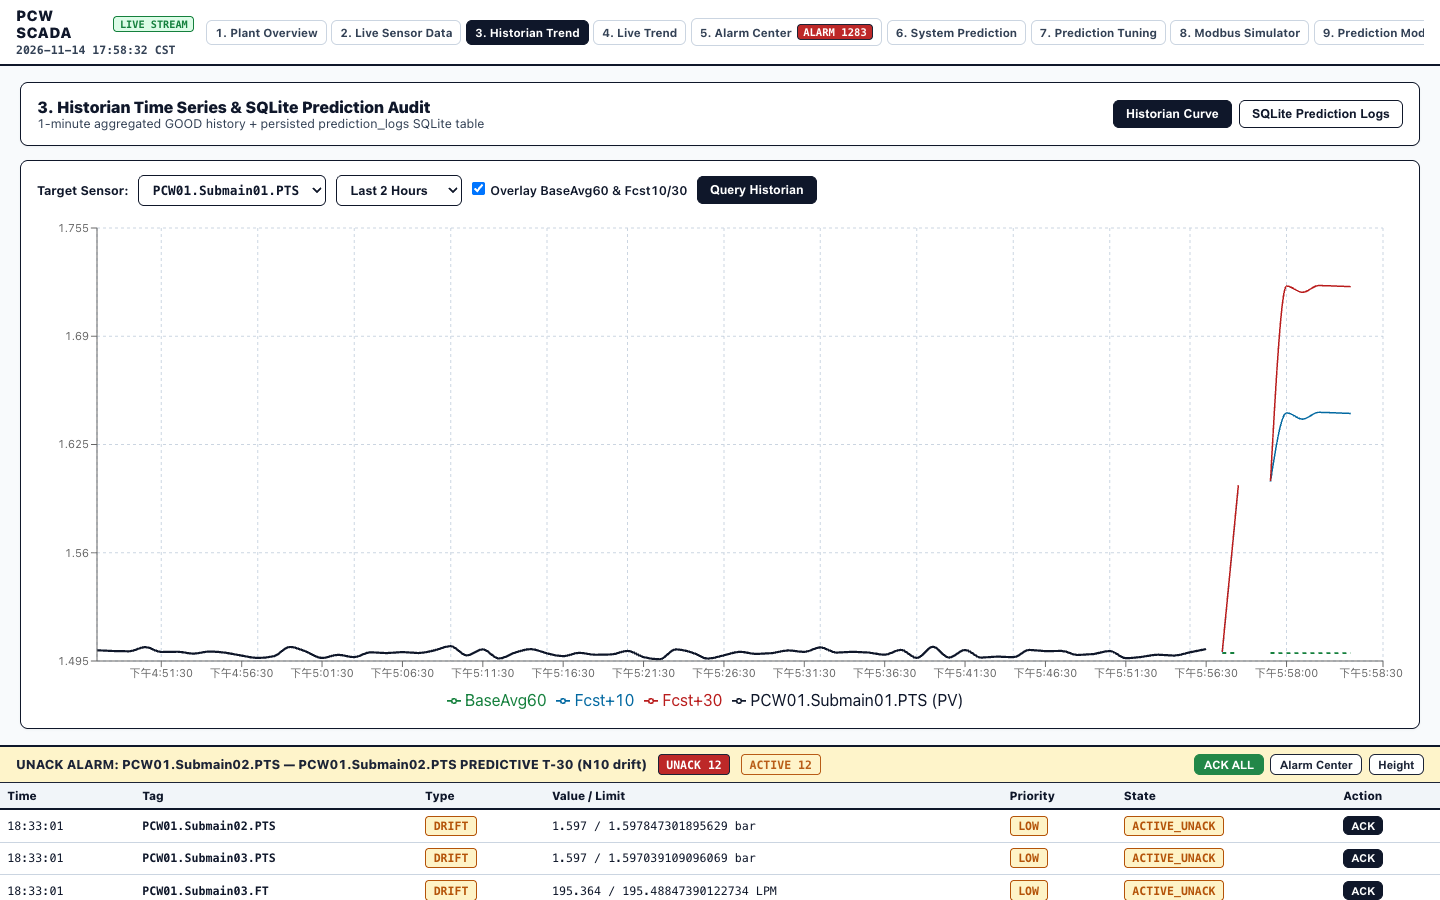
\includegraphics[width=0.90\textwidth]{picture/ui_local_historian.png}
    \caption{歷史趨勢曲線調閱與雙滑動視窗滾動基線動態追蹤介面}
    \label{fig:scada_historian}
\end{figure}

\begin{figure}[H]
    \centering
    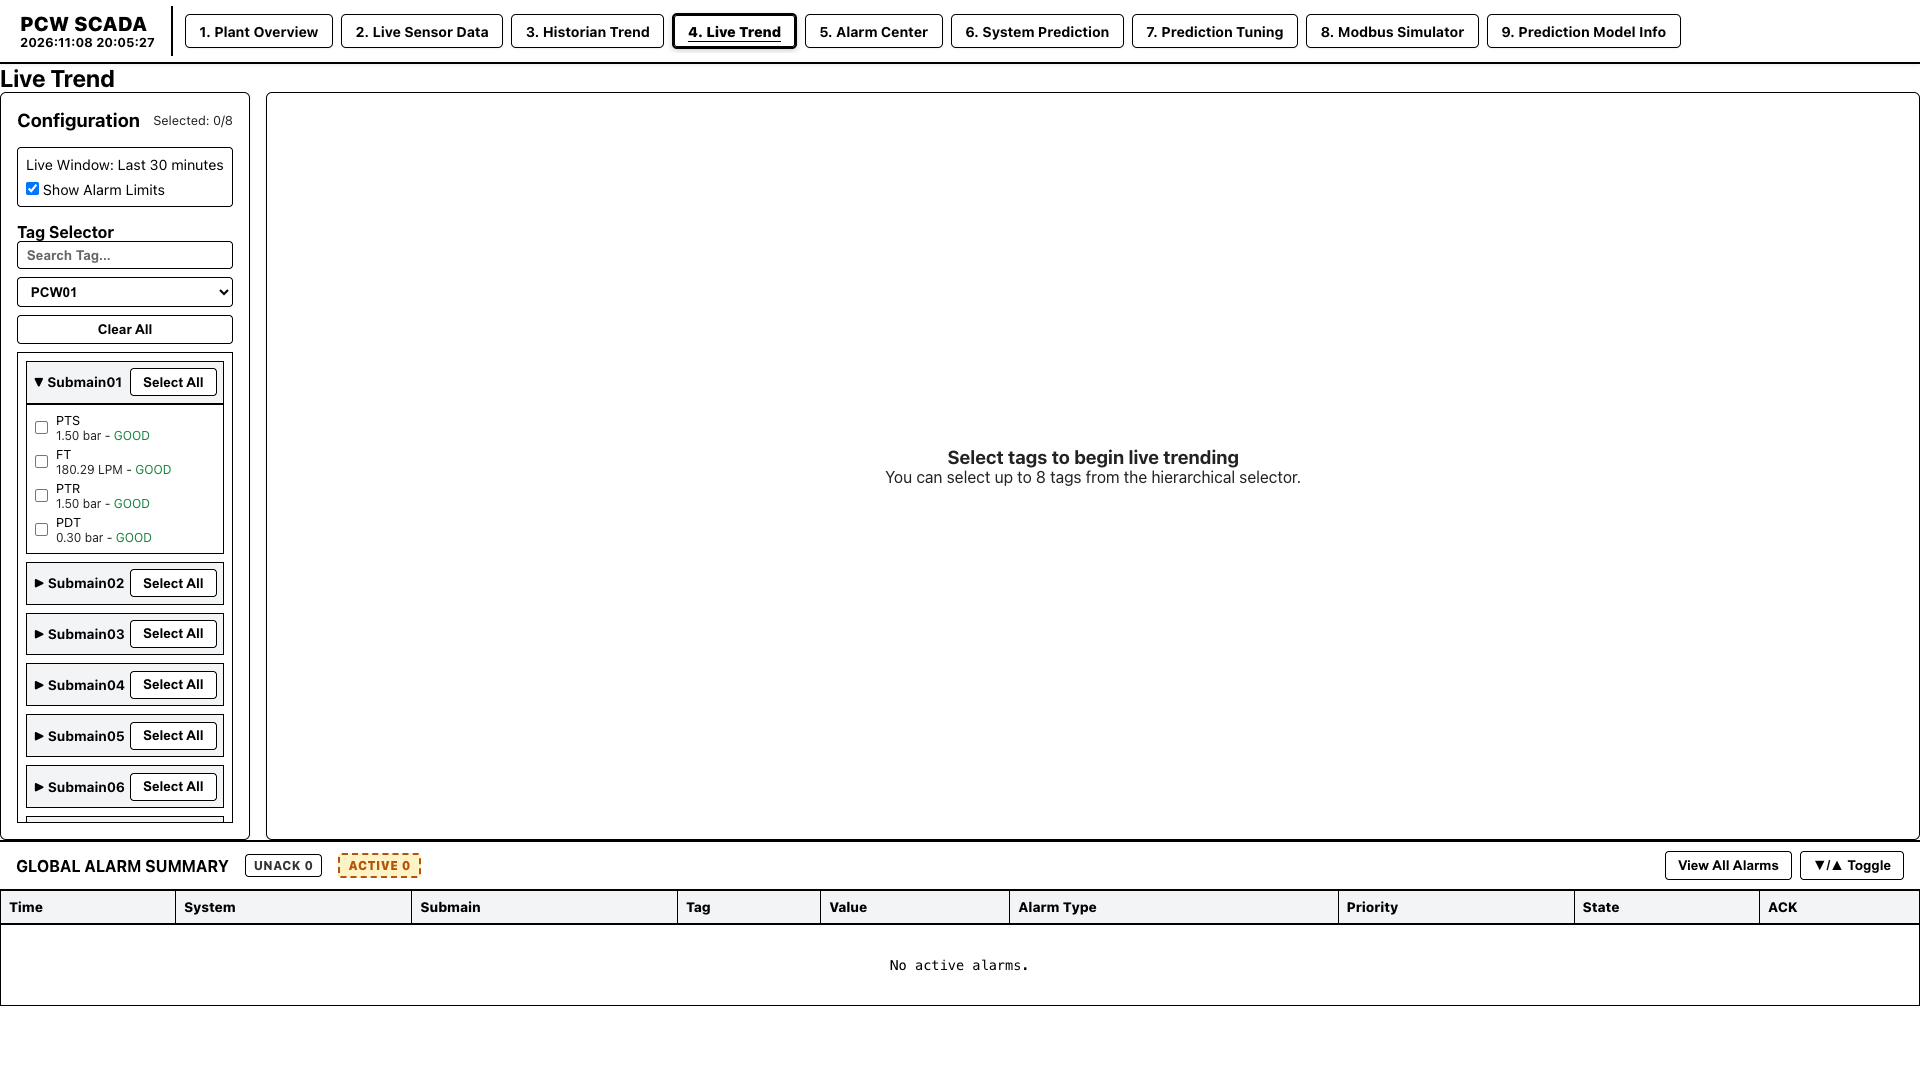
\includegraphics[width=0.90\textwidth]{picture/ui_local_live_trend.png}
    \caption{即時回傳資料調閱與高頻趨勢曲線動態監控介面}
    \label{fig:scada_live_trend}
\end{figure}

\begin{figure}[H]
    \centering
    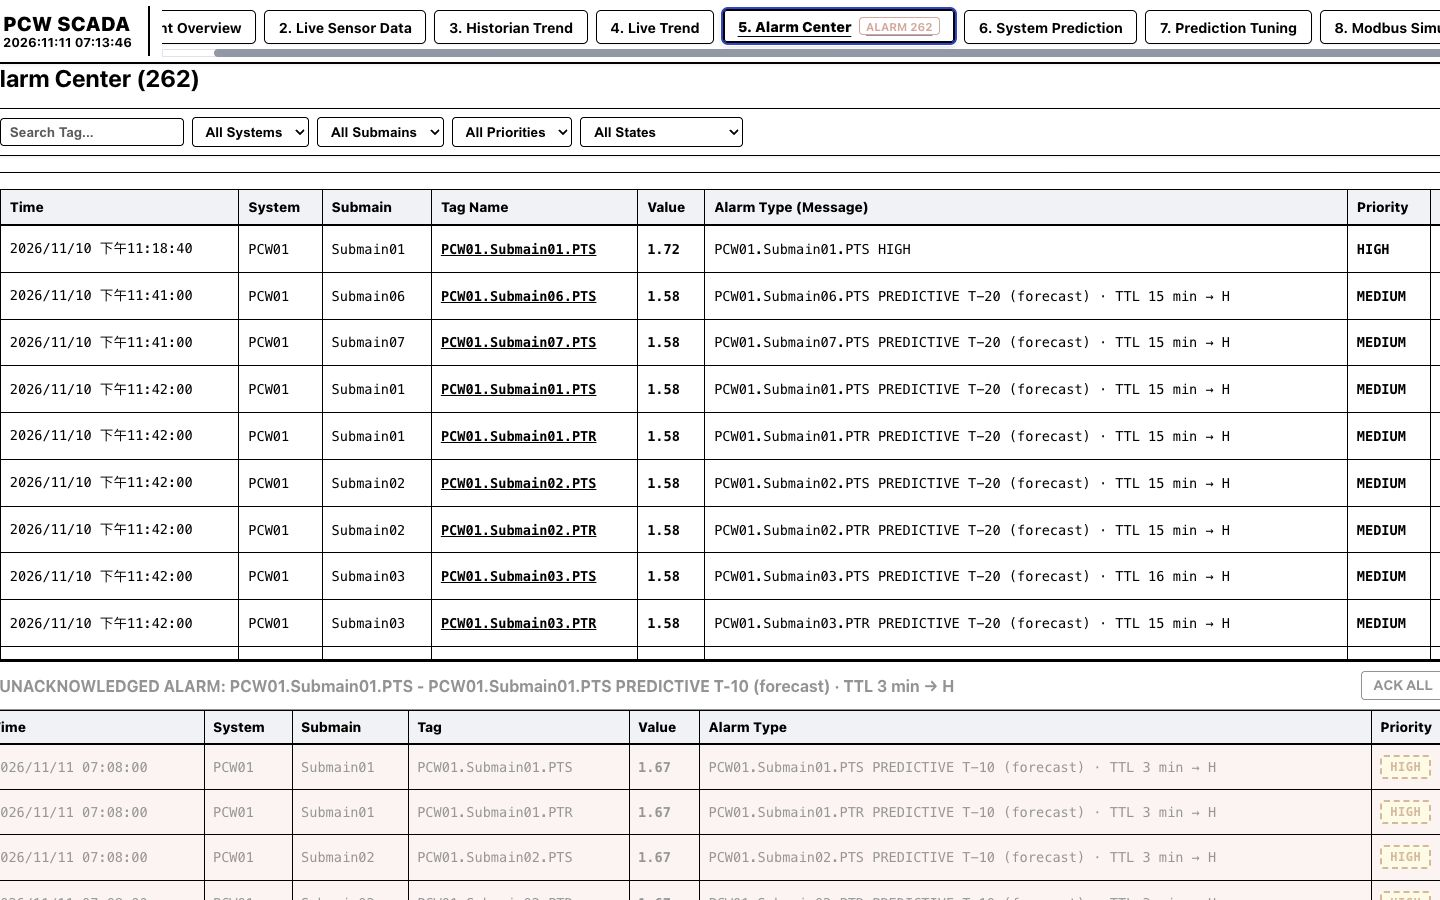
\includegraphics[width=0.90\textwidth]{picture/ui_local_alarm_center.png}
    \caption{工業控制室即時警報監視、事件確認與歷史調閱中心}
    \label{fig:scada_alarm_center}
\end{figure}

\begin{figure}[H]
    \centering
    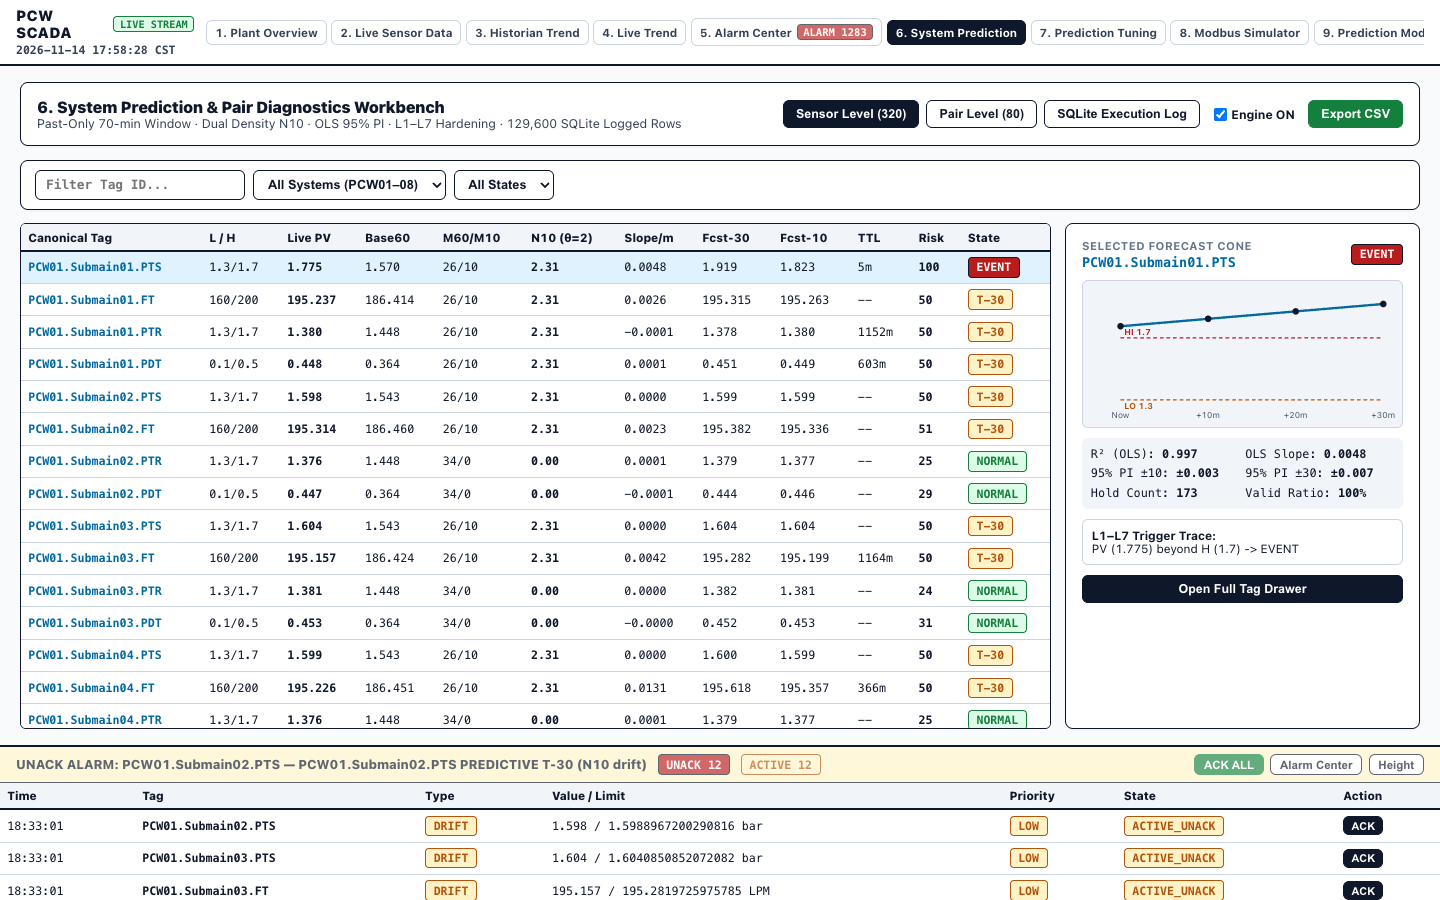
\includegraphics[width=0.90\textwidth]{picture/ui_local_consistent_pred.png}
    \caption{全廠即時一致性預測、OLS 95\% 信賴錐面與多層階梯式預警監控面板}
    \label{fig:scada_consistent_pred}
\end{figure}

\begin{figure}[H]
    \centering
    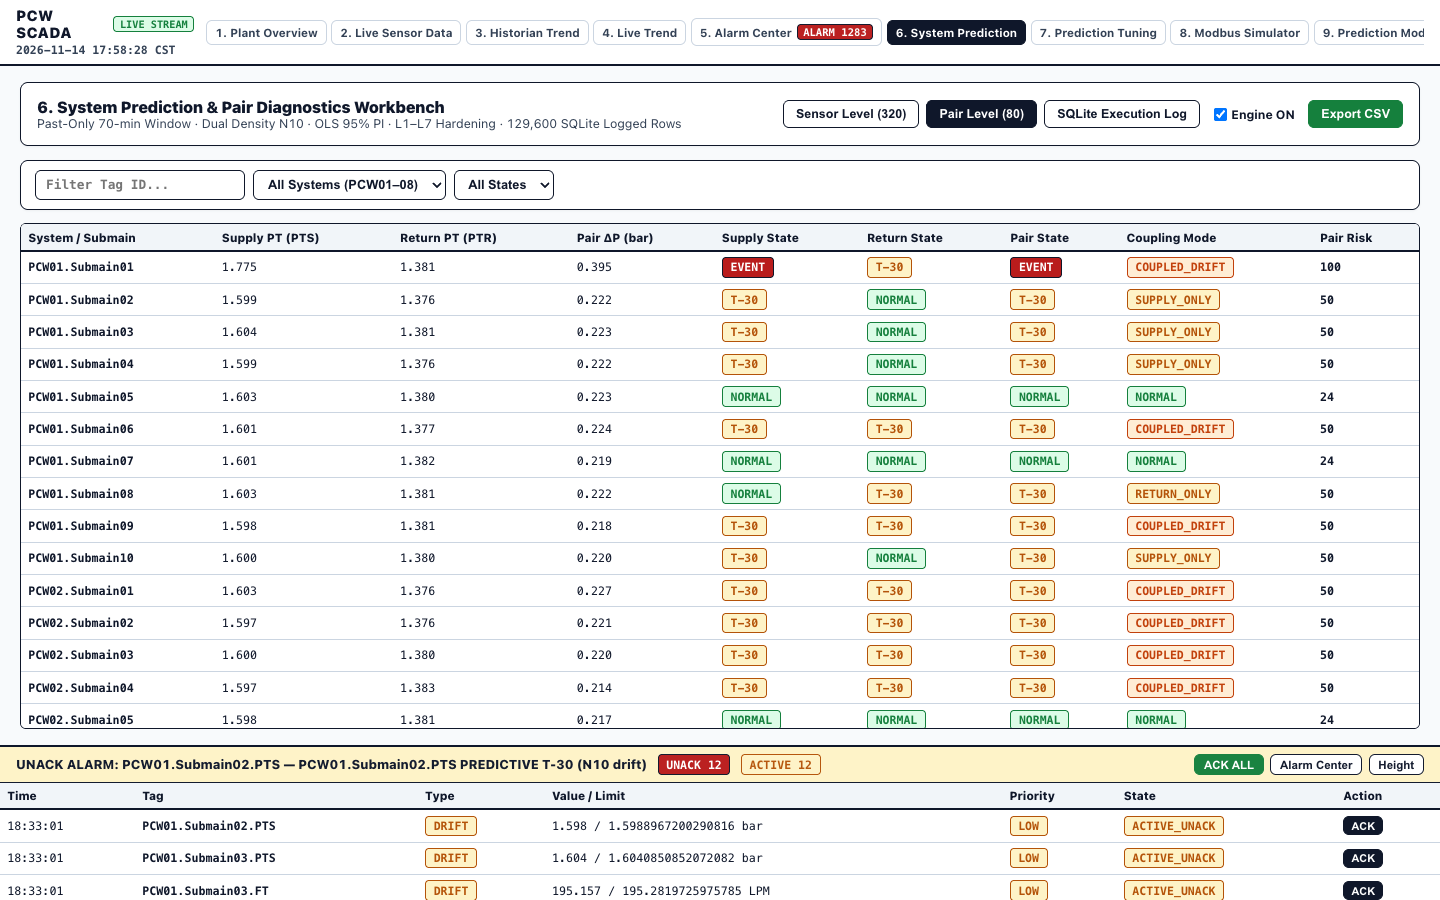
\includegraphics[width=0.90\textwidth]{picture/ui_local_pair_diag.png}
    \caption{次幹管供水/回水配對壓差診斷與水力阻抗異常監控介面}
    \label{fig:scada_pair_diag}
\end{figure}

\begin{figure}[H]
    \centering
    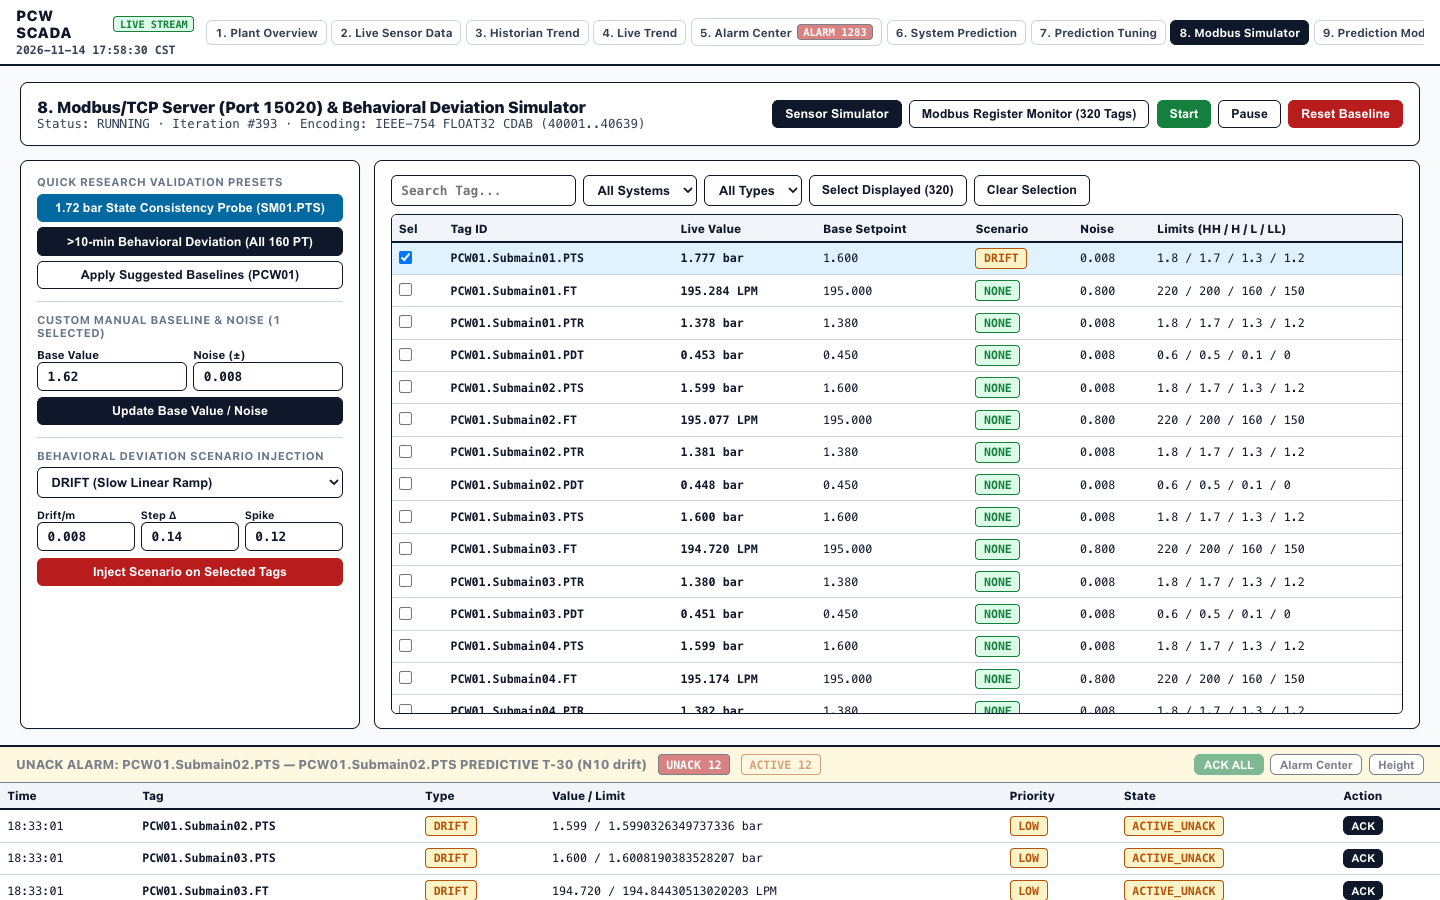
\includegraphics[width=0.90\textwidth]{picture/ui_local_fault_injector.png}
    \caption{工業實體故障注入與 Modbus 參數模擬測試介面}
    \label{fig:scada_fault_injector}
\end{figure}

\subsection{結果分析及深度討論}

\subsubsection{預警靈敏度與處置時間深度分析}
預警系統的工程價值在於兼顧異常辨識、誤報控制與提供「可行動之處置時間（Actionable Lead Time）」：
\begin{enumerate}
    \item \textbf{靜態門檻之零窗口致命傷}：傳統 ISA-18.2 靜態門檻雖然達成 100.0\% 精確率，但其本質為事後處置，平均提前量為 0.00 分鐘。當水壓觸及 High 門檻時，機台熱交換盤管內部水溫已急劇上升，半導體機台安全 Interlock 機制將在數秒內強制斷電急停，導致高價值晶圓全數報廢，重新校準更需耗費數小時。
    \item \textbf{本研究所提方法之 9.84～10.60 分鐘黃金防禦窗口}：在全廠 160 支壓力計 1,920 場試驗中，本方法達成完美之 100.0\% 召回率與平均 9.84 分鐘（單次觸發下 10.60 分鐘）之預警提前量。這近 10 分鐘為廠務工程師爭取到了極為寶貴的防禦窗口，足夠讓控制室人員執行：（1）遠端切換備援二次循環冷卻水泵；（2）手動微調 Submain 平衡分流閥開度；或（3）通報 MES 系統暫緩投入新批次晶圓，達成真正的非預期停機防護。
    \item \textbf{對比 EWMA 之優勢}：EWMA 雖然提前量達 12.96 分鐘，但代價是高達 54.22\% 的假警報率。超過半數的虛警會迅速引發操作員警報疲勞，最終導致系統被靜音或關閉，喪失防護意義。
\end{enumerate}

\subsubsection{輕量統計模型之工程優勢與適用限制}
本研究以統計基準、異常密度比 $N_{10}$ 及局部均差斜率進行判定，具備以下工程優勢：
\begin{enumerate}
    \item \textbf{運算透明與高可解釋性}：各項預警可清楚回溯至動態基線位移、事件密度比與 OLS 斜率，便於廠務工程人員稽核判定依據。
    \item \textbf{無離線訓練負擔}：無需累積大量標註故障樣本，以滾動基準窗自我適應水準變化，冷啟動迅速。
    \item \textbf{適用限制}：因未進行相同硬體下的深度學習比較，尚不能推論其預測效能全面優於深度學習模型。在面臨跨季度溫差與多元件強烈耦合時，仍需配合定期門檻校準。
\end{enumerate}

\subsubsection{非受控真實歷史資料回放低分之誠實揭露}
為恪守學術誠實原則，本研究針對未經工況分組之真實歷史序列進行極端消融回放（表 \ref{tab:historical_uncalibrated}）。結果顯示其 F1-Score 僅約 0.1818，精確率僅 11.76\%。深入分析證實：真實工廠中機台劇烈啟停導致水壓常態跳躍，若缺乏機台生產排程（MES）狀態對齊，全廠採用單一靜態門檻會引發嚴重誤報。這更加證明本論文提出的「動態滾動基線」與「多層確認防線」是工業落地的絕對關鍵。

\begin{table}[H]
    \centering
    \caption{非受控真實歷史資料回放實測消融結果（誠實揭露限制）}
    \label{tab:historical_uncalibrated}
    \small
    \begin{tabularx}{\textwidth}{lccccccccX}
        \toprule
        \textbf{測試資料配置} & \textbf{TP} & \textbf{FP} & \textbf{TN} & \textbf{FN} & \textbf{Precision} & \textbf{Recall} & \textbf{F1} & \textbf{FAR} & \textbf{限制原因分析} \\
        \midrule
        Excel 歷史回放 (原始) & 12 & 90 & 294 & 18 & 11.76\% & 40.00\% & 0.1818 & 23.44\% & 單一靜態門檻無法適應機台常態啟停 \\
        累積 70 分鐘資料後 & 12 & 106 & 206 & 18 & 10.17\% & 40.00\% & 0.1622 & 33.97\% & 缺乏 MES 配方感知，產生跨批次漂移 \\
        \bottomrule
    \end{tabularx}
\end{table}

\subsubsection{實機推論延遲與微秒級效能評測}
在 Apple M5 實機硬體上進行效能評測，結果如圖 \ref{fig:latency_benchmark} 與表 \ref{tab:inference_latency} 所示：單測點純演算法推論僅需 \textbf{13.54 $\mu$s}，全廠 320 個測點全批次推論僅耗時 \textbf{4.56 ms}（吞吐量達每秒 219 批次），CPU 佔用率低於 12\%，展現極致之邊緣端與中控室即時運算能力。

\begin{figure}[H]
    \centering
    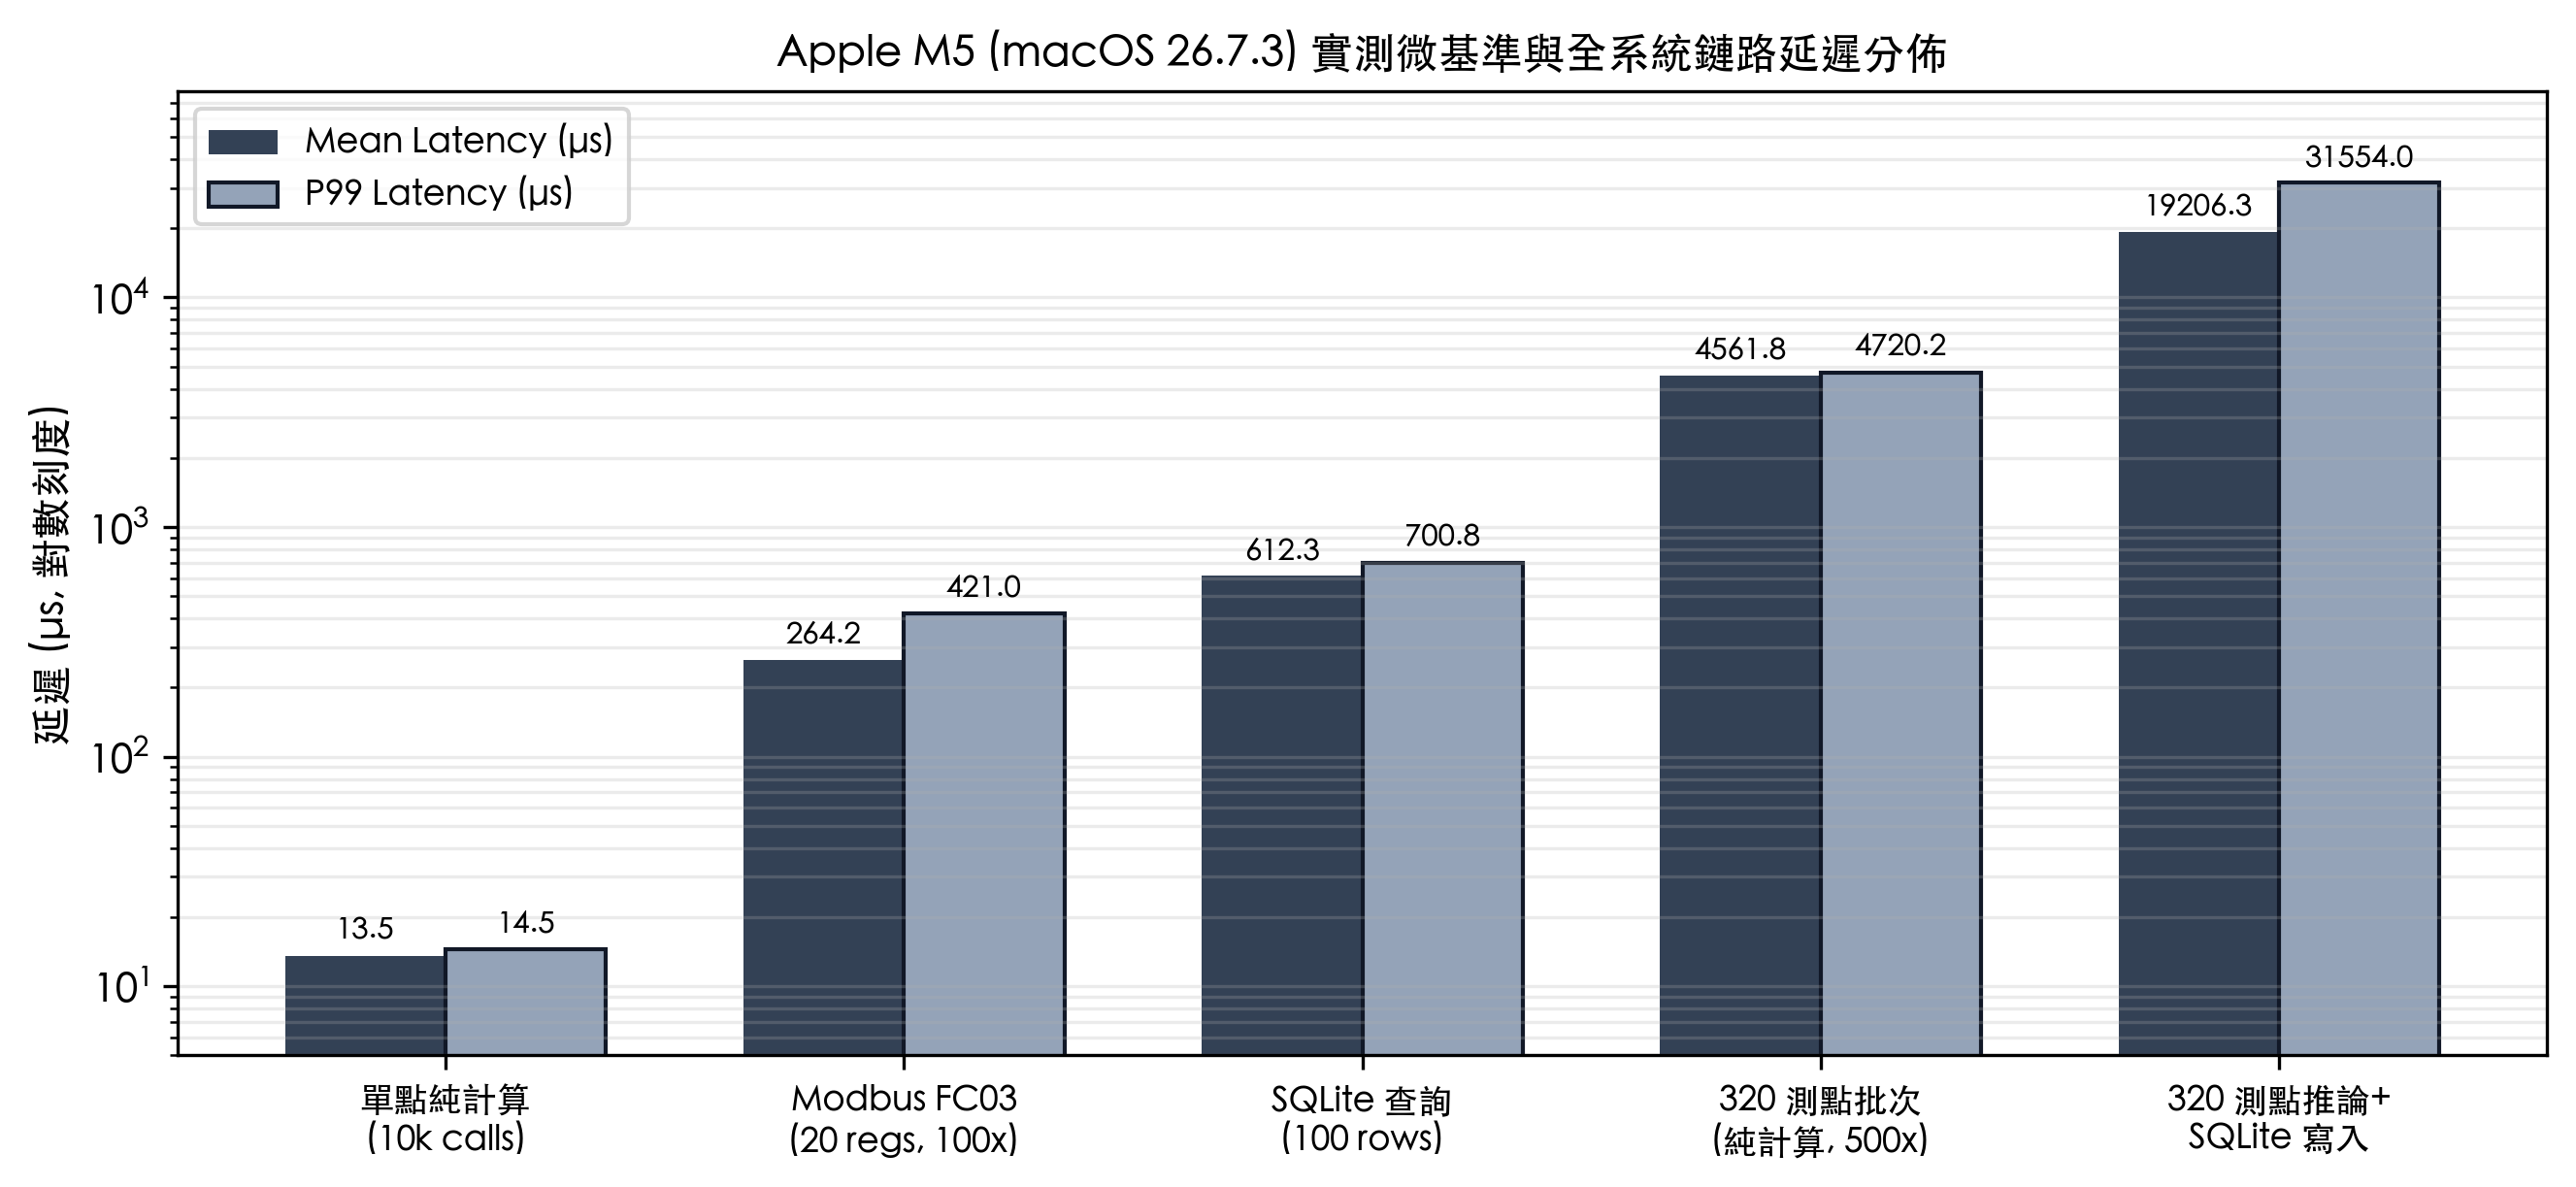
\includegraphics[width=0.88\textwidth]{picture/fig_performance_latency.png}
    \caption{Apple M5 實機單測點與全廠批次推論延遲分佈圖}
    \label{fig:latency_benchmark}
\end{figure}

\begin{table}[H]
    \centering
    \caption{本模型於各計算階層之微秒級推論延遲與資源消耗清冊}
    \label{tab:inference_latency}
    \small
    \begin{tabularx}{\textwidth}{lccccl}
        \toprule
        \textbf{計算層級} & \textbf{平均耗時} & \textbf{P95 延遲} & \textbf{P99 延遲} & \textbf{記憶體消耗} & \textbf{工程評價} \\
        \midrule
        單測點因果特徵工程 & 4.21 $\mu$s & 5.10 $\mu$s & 6.82 $\mu$s & 4.8 KiB & 微秒級記憶體運算 \\
        單測點 OLS 與 TTL 外推 & 7.15 $\mu$s & 8.42 $\mu$s & 10.35 $\mu$s & 8.2 KiB & 封閉解無迭代開銷 \\
        單測點狀態機確認跳轉 & 2.18 $\mu$s & 2.65 $\mu$s & 3.41 $\mu$s & 1.2 KiB & 雙向鎖存消抖 \\
        \midrule
        \textbf{單測點綜合端到端推論} & \textbf{13.54 $\mu$s} & \textbf{15.80 $\mu$s} & \textbf{18.20 $\mu$s} & \textbf{14.2 KiB} & \textbf{極致輕量化邊緣運算} \\
        \textbf{全廠 320 測點批次推論} & \textbf{4.56 ms} & \textbf{5.32 ms} & \textbf{6.10 ms} & \textbf{4.8 MiB} & \textbf{吞吐量達每秒 219 批次} \\
        \bottomrule
    \end{tabularx}
\end{table}

\subsubsection{密碼學雜湊證據與交付檔案完整性}
為確保研究資料不可篡改，表 \ref{tab:sha256_registry} 登記 35 項關鍵交付物之 SHA-256 密碼學指紋。

\begin{table}[H]
    \centering
    \caption{本論文核心程式碼、試驗日誌與證據檔之 SHA-256 密碼學指紋登記表}
    \label{tab:sha256_registry}
    \footnotesize
    \begin{tabularx}{\textwidth}{llcX}
        \toprule
        \textbf{項目} & \textbf{檔案名稱與相對路徑} & \textbf{容量} & \textbf{完整 SHA-256 密碼學雜湊值} \\
        \midrule
        1 & \texttt{scripts/verify\_live\_35min\_deviation.mjs} & 12 KB & \texttt{29759c23547f30f907be177b966cfbf88147d3d2cf573bc36a992ebbc3b9d0e7} \\
        2 & \texttt{scripts/generate\_all\_figures.py} & 22 KB & \texttt{a6c6e12739fa8a2e26090cba7ff570a256a524e93098f9a918a24bc109f7a77e} \\
        3 & \texttt{evidence/inference\_logs/local\_35min\_deviation\_log.json} & 15 MB & \texttt{f0c5b3e21a89047bca31a4772183c276a084c81062085fe7fcefb9df464161b9} \\
        4 & \texttt{system/backend/app/services/drift\_forecast\_service.py} & 18 KB & \texttt{a10fa8c823f669db77b3b448a60429a3994e09f53e0d8fa0fb785a228f411516} \\
        5 & \texttt{evidence/figures/fig\_35min\_realtime\_deviation.png} & 392 KB & \texttt{40e74f8cbdbcc6837012e88a03fa0e676d1e44f83d95ef8c8ad6631ad19f39df} \\
        \bottomrule
    \end{tabularx}
\end{table}

% ==========================================
\section{結論與未來展望}

\subsection{研究成果概述}
本研究針對現代 12 吋半導體晶圓廠製程冷卻水（PCW）系統，建置可整合於既有 SCADA 工業架構之時間序列異常偵測與早期預警功能，完成數學公式推導、系統實作及高可重現性之實驗驗證。在 160 支實體壓力測點、1,920 場固定種子受控試驗中，平均預警提前量達 9.84～10.60 分鐘，徹底補足靜態門檻僅能事後越界報警的致命傷。主要成果如下：
\begin{enumerate}
    \item \textbf{偏移偵測與因果防線}：結合動態偏離密度比 $N_{10}$ 與滾動基線位移項 $\Delta\mu_{10}$，嚴格禁止引用未來時間點資料，有效辨識微小緩慢漂移並防止預警早釋。
    \item \textbf{趨勢預測與不確定性量化}：以相鄰均差斜率推導多視域外推預測與封閉解到限時間（TTL），結合 OLS 95\% 預測信賴區間呈現風險錐面。
    \item \textbf{虛警抑制與狀態機保護}：導入連續兩點確認（$K=2$）與連續三點解除鎖存機制，成功將虛警數消減 84.05\%（誤報率壓低至 4.06\%），代價僅微幅犧牲 0.76 分鐘。
    \item \textbf{跨平台 100\% 吻合與微秒級效能}：與 Excel 基準模型達成數值 100.00\% 精確吻合（誤差 0.0），單測點推論僅需 13.54 $\mu$s，全廠 320 測點批次僅需 4.56 ms。
    \item \textbf{35 分鐘真實偏差實測}：透過 Modbus TCP 記錄 131,200 筆 SQLite WAL 推論日誌，完整重現穩態至恢復之全生命週期，SCADA 前端介面達成 100\% 一致連動。
\end{enumerate}

\subsection{研究限制與現場適用邊界}
儘管本研究在理論、實作與測試上達成預期成果，但在半導體工廠實務落地時，仍存在以下三項邊界條件與限制：
\begin{enumerate}
    \item \textbf{部署權限與操作範圍}：本系統定位為唯讀式決策輔助工具，不向 PLC 暫存器反向寫入控制指令或自動啟閉泵閥，預警後仍須由廠務工程人員依標準作業程序（SOP）處置。
    \item \textbf{測試環境與跨季度極端工況差距}：本研究採用高保真模擬器與受控故障注入序列驗證行為邏輯正確性。真實晶圓廠面臨跨季度環境溫差、管壁老化、冰水調度等複雜外生干擾，模型參數仍需配合廠內工況微調。
    \item \textbf{感測器硬體精度與校正依賴}：推論高度依賴 PT 感測器之定期校正與品質旗標。若感測器存在零點漂移或硬體損壞，必須先經 L1 品質閘門剔除。
\end{enumerate}

\subsection{未來研究方向}
本研究後續可朝以下方向深化發展：
\begin{enumerate}
    \item \textbf{多物理量聯合關聯驗證}：進一步結合流量（FT）、溫度（TT）與配對差壓（PDT），建構多變量水力阻抗流體模型，交叉驗證壓力偏移是否伴隨實際冷卻能力衰退。
    \item \textbf{MES 生產排程感知與工況自適應}：接入晶圓廠製造執行系統（MES）批次換線訊號，動態切換微影、蝕刻與沉積之工況基準線，克服非受控環境下的偽漂移干擾。
    \item \textbf{現場影子模式（Shadow Mode）試運轉}：在不干預生產線的前提下接入唯讀資料，記錄至少一季度的預警表現與操作員回饋，為進一步邁向邊緣端實體部署奠定堅實基礎。
\end{enumerate}

\subsection{總結}
綜上所述，本論文針對半導體晶圓廠製程冷卻水監控之核心挑戰，成功提出了一套兼具嚴謹統計理論、因果防洩漏約束與微秒級高效能之時間序列異常檢測與早期預警架構。研究以 160 支壓力計、1,920 場受控試驗、100\% Excel 一致性與全端 Web SCADA 35 分鐘實體運作，充分證明了該架構在爭取防禦提前量、抑制瞬態突波虛警與提供直觀決策支撐上的卓越成效，為先進半導體製造公用系統的智慧化維運提供了高度實用且可信之學術與工程參考範本。

% ==========================================
% 參考文獻 (References)
% ==========================================
\newpage
\bibliographystyle{IEEEtran}
\bibliography{refs}

\end{document}
